% !TeX encoding = UTF-8
% !TeX spellcheck = en_GB
\documentclass[a4paper, 11pt]{article}
%\documentclass[a4paper, 12pt]{article}
\usepackage[utf8]{inputenc}

%margin
\usepackage[margin=2cm]{geometry}
%\usepackage[margin=1in]{geometry}
\usepackage{changepage}
%line spacing
\renewcommand{\baselinestretch}{1.15}
%\renewcommand{\baselinestretch}{1.6}
%lists
\usepackage{enumitem}
%multi-columns
\usepackage{multicol}
%encoding
\usepackage[utf8]{inputenc}
\usepackage[T1]{fontenc}
%English
\usepackage[english]{babel}
%colors
\usepackage[dvipsnames,svgnames,table]{xcolor}
%tables
\usepackage{multirow}
\usepackage{longtable}
\usepackage{tabularx}
%for math
\usepackage{amsfonts}
\usepackage{amssymb}
\usepackage{mathrsfs}
\usepackage{amsmath}
\usepackage{amsthm}
\usepackage{mathtools}
\usepackage{mathdots}
\usepackage{nicefrac}
\usepackage{stmaryrd}
\usepackage{makecell}
%for images
\usepackage{graphicx}
\usepackage{caption}
\usepackage{subcaption}
\usepackage{wrapfig}
\graphicspath{{./img/}{./plots/}{./crossings/}}
%for plots
\usepackage{tikz}
\usepackage{adjustbox}
%links
%\usepackage[hyphens]{url}
\usepackage{hyperref}
%\hypersetup{colorlinks=true}
%citations
\bibliographystyle{unsrtnat}
%code
\usepackage{minted}
%\usepackage[cache=false]{minted}
%\usepackage{listings}
\usepackage{algorithm}
\usepackage{algpseudocode}
\definecolor{CodeColor}{RGB}{100, 100, 100}


%environments
\newtheorem*{notation}{Notation}
\newtheorem{definition}{Definition}[section]
\newtheorem*{claim}{Claim}
\newtheorem{proposition}{Proposition}[section]
\newtheorem{property}{Property}[section]
\newtheorem{lemma}{Lemma}[section]
\newtheorem{theorem}{Theorem}
\newtheorem{corollary}{Corollary}[section]
\newtheorem*{conjecture}{Conjecture}
%commands
%\newcommand{\name}[num]{definition}
\newcommand{\primes}{\mathbb{P}}
\newcommand{\N}{\mathbb{N}}
\newcommand{\Z}{\mathbb{Z}}
\newcommand{\Q}{\mathbb{Q}}
\newcommand{\D}{\mathbb{D}}
\newcommand{\R}{\mathbb{R}}
\newcommand{\C}{\mathbb{C}}
\newcommand{\F}{\mathbb{F}}
\newcommand{\halfplane}{\mathbb{H}}
%\newcommand{\dim}[1]{\text{dim}(#1)}
\newcommand{\SL}[2]{\text{SL}_{#1}(#2)}
\newcommand{\Norm}[2][]{\text{Norm}_{#1}(#2)}
\newcommand{\floor}[1]{\lfloor #1 \rfloor}
\newcommand{\ceil}[1]{\lceil #1 \rceil}
\newcommand{\abs}[1]{| #1 |}
\newcommand{\curt}[1]{\sqrt[3]{#1}}
\newcommand{\Ker}[1]{\text{Ker}(#1)}
\newcommand{\Image}[1]{\text{Im}(#1)}
\newcommand{\Gal}[1]{\text{Gal}(#1)}
\newcommand{\Frob}[2]{\text{Frob}_{#1}(#2)}
\newcommand{\Tr}[1]{\text{Tr}(#1)}
\newcommand{\Det}[1]{\text{Det}(#1)}
\newcommand{\End}[1]{\text{End}(#1)}
\newcommand{\Aut}[1]{\text{Aut}(#1)}
\newcommand{\legendre}[2]{\left( \frac{#1}{#2} \right)}
\newcommand{\degree}[1]{\partial #1}
\newcommand{\diam}[1]{\text{diam}(#1)}




\begin{document}
	\begin{titlepage}
	\newcommand{\HRule}{\rule{\linewidth}{0.5mm}}
		\begin{center}
		
\includegraphics[scale=0.08]{oxford_logo.png}
		\vspace*{1cm}
		
		\textsc{\LARGE University of Oxford}\\[0.75cm]
		\textsc{\LARGE Mathematical Institute}
		
		\vspace{1.5cm}
		
		\HRule

		\vspace{0.5cm}

		\textbf{\huge Random Fractals:\\}
		\vspace{0.3cm}
		\textbf{\huge Traversing without Zebra Crossing}
		
		\vspace{0.5cm}
		\HRule
		
		\vspace{1.5cm}
		
		\begin{minipage}{0.4\textwidth}
			\begin{flushleft}
				\large
				%\textit{Author}\\ Paul \textsc{Dubois}
			\end{flushleft}
		\end{minipage}
		
		\begin{minipage}{0.4\textwidth}
			\begin{flushright}
				\large
				%\textit{Supervisor}\\ Ben \textsc{Hambly}
			\end{flushright}
		\end{minipage}
		
		\vspace{0.5cm}
		
		\textit{Candidate Number}\\
		1051774
		
		\vspace{0.5cm}
		
		\textit{Course}\\
		MSc Mathematical Sciences
		
		\vfill
		
		{\large Trinity Term\\
			April 26, 2021}
	\end{center}
\end{titlepage}

	\footnotetext{Title inspired of the pseudo-joke "Why did the chicken cross the road?" (see \url{https://en.wikipedia.org/wiki/Why_did_the_chicken_cross_the_road\%3F}).}
	\begin{center}
		\LARGE Percolation Fractals
	\end{center}
	\vspace{0.5cm}
	\begin{abstract}
		Percolations are geometric figures obtained after repetitively removing some material from an initial set, in our case, a cuboid.
		Studying their properties provide a better understanding of some physical models for materials: some porous materials are modelled using percolations.
		In this paper, we study mathematical properties of percolations starting with cuboids of any dimensions, and make numerical experiments on the two and three dimensional cases.
		
		We will introduce the concept of dimensionality for sets, and the concept of fractal.
		We will then narrow down our interest to a special type of fractals: the one obtained by percolation.
		Two competing models will be studied: the classical percolation, and the recursive scheme.
		
		After discussing some basic properties (density, dimension, size of the central "blob"), we will look at crossings on percolations.
		This is the main purpose of this paper, we will derive some mathematical result in extreme cases, and use some innovative algorithms to obtain relevant numerics.
		Finally, we will extend techniques used in previous literature for percolations in two dimensions to acquire knowledge in more general settings. 
	\end{abstract}
	
	\vspace{2.5cm}
	\begin{center}
		\textbf{Acknowledgment}
	\end{center}
	{
		\small
		\hspace{1cm}
		First of all, I would like to thank my supervisor, Ben Hambly, for guiding and supporting through this project.
		I would like to thank the whole administrative team of Oxford, for all the help they provided despite the pandemic context.
	}

	\vspace{2.5cm}
	\begin{center}
		\textbf{Word Count}
	\end{center}
	\begin{center}
		%\textit{Word count by Overleaf}
		\begin{tabular}{r l}
			Total Words: & 7432 \\
			Headers: & 87 \\
			Math Inline: & 618 \\
			Math Display: & 29 \\
			Figures: & 38 \\
			Algorithms: & 2 \\
		\end{tabular}
	\end{center}
	
	\newpage
	
	\tableofcontents
	
	% !TeX spellcheck = en_GB
\setcounter{section}{-1}
\section{Introduction}


	% !TeX spellcheck = en_GB
\section{Background Theory}
We derive here a mathematical basis on fractals and dimensions of sets.
This will be used later in our more specific study of random fractals.

\subsection{Dimensions}
The concept of dimension is quite intuitive from an everyday life perspective.
However, the mathematical concept is more involved.
From the non-mathematical world, this can be used to have better understanding of other object arising from other fields such as DNA structure\footnote{\url{https://news.mit.edu/2009/3d-genome}}, or lungs\cite{IOLMSD_2009}.

\subsubsection{Intuition}
Some objects that we are used to working with have an established dimension:
\begin{itemize}
	\item \textbf{Empty set} / \textbf{Point}: dimension 0
	\item \textbf{Curve} (e.g.: \textit{line}): dimension 1
	\item \textbf{Surface} (e.g.: \textit{square}): dimension 2
	\item \textbf{Volume} (e.g.: \textit{cube}): dimension 3
	%\item \textbf{General $d$-dim set} (e.g.: \textit{$d$-dimensional cuboid}): dimension $d$
\end{itemize}
All of these usual objects have integral dimensions, making it (relatively) easy to understand.

A rule of thumb to calculate the dimension is to double (or, in general, multiply by $n$) the size of the object, and count the number of copies of the original object obtained.
If there are $N$ original objects, the dimension is $d = \frac{\ln(N)}{\ln(n)}$.
This is so that when scaling by $n$, the length/area/volume of the set is multiplied by $N = n^d$.

Some objects have a more complicated dimension (in fact, a non-integral one)\footnote{This will be discussed in more detail in \ref{fractalsExamples}.}:
\begin{itemize}
	\item \textbf{Cantor Set} (see fig. \ref{fig:CantorSet}): dimension $\log_3(2) = \frac{\ln(2)}{\ln(3)} \simeq 0.631$
	\item \textbf{Koch Snowflake} (see fig. \ref{fig:KochSnowflake}): dimension $\log_3(4) = \frac{\ln(4)}{\ln(3)} \simeq 1.262$
	\item \textbf{Sierpiński Carpet} (see fig. \ref{fig:SierpinskiCarpet}): dimension $\log_2(8) = \frac{\ln(8)}{\ln(3)} \simeq 1.893$
\end{itemize}
The fractional dimensions of these objects justify creating a formal mathematical definition.

After this quick overview, 3 properties seem desirable for a definition of dimension \cite{Pollicott_LFDT}.
For a set $X$ ($\subset \R^n$, in general):
\begin{enumerate}\label{propr:desirable}
	\item If $X$ is a manifold, then the dimension should coincide with our natural preconception. \label{propr:desirable1}
	\item In some cases, $X$ may have a fractional (i.e. non-integral) dimension. \label{propr:desirable2}.\\
	This is needed in order to describe sets as the ones discussed above.
	\item If $X$ is countable, then $X$ has dimension $0$. \label{propr:desirable3}
\end{enumerate}
There are several definition for dimension, satisfying different properties.

\subsubsection{Topological Dimension}
The topological dimension is the most straightforward way to define dimension.
It relies on the intuition that the boundary of a ball of dimension $d$ should have dimension $d-1$.

\begin{definition}[Topological dimension]\label{def:topologicalDimension}
	The topological dimension $\dim_T(X)$ of a set $X$ is defined recursively through the following:
	\begin{equation*}
		\dim_T(X) =
		\begin{cases}
			-1 & \text{if } \ X = \emptyset \\
			 d & \text{if } \ d = \min \left\lbrace n \in \N \mid \forall x \in X, \ \exists \, r>0 \text{ s.t. } \dim_T(\partial B_r(x) \cap X) \leq n-1 \right\rbrace
		\end{cases}
	\end{equation*}
\end{definition}

This definition satisfies the first desired property (\ref{propr:desirable}:\ref{propr:desirable1}).
However, $\dim_T$ is always an integer (this is clear from definition).
Therefore, it does not satisfy the second desired property (\ref{propr:desirable}:\ref{propr:desirable2}).

\subsubsection{Box Dimension}
The box dimension is more general than the topological one, in the sense that it allows non-integral dimensions.
It relies on an intuition mentioned before: when scaled by $n$, a set contains $N$ copies of the original set, then the dimension should be  $\frac{\ln(N)}{\ln(n)}$.

\begin{definition}[Box dimension]\label{def:boxDimension}
	The box dimension $\dim_B$ of a set $X$ is defined through the following limit:
	$$
	\dim_B(X) = \lim_{\varepsilon \to 0} \frac{\ln(N(\varepsilon))}{-\log(\varepsilon)}
	$$
	Here, $N(\varepsilon)$ is the smallest number of $\varepsilon$-balls needed to cover $X$.
	
	Note that box dimension exists only if this limit exists.
	In the case this limit does not exist, it is possible to define upper and lower box dimensions, taking respectively $\limsup$ and $\liminf$ in the definition above.
	(Both upper and lower box dimension with the general box dimension when it exists.) 
\end{definition}

This definition satisfies the first and second desired property (\ref{propr:desirable}:\ref{propr:desirable1},\ref{propr:desirable2}).
However, if we consider $X = \{0\} \cup \{\frac{1}{n} \mid n \in \N^*\}$, then $\dim_B(X) > 0$, but $X$ is countable.
Therefore, it does not satisfies the third desired property (\ref{propr:desirable}:\ref{propr:desirable3}).

\subsubsection{Hausdorff Dimension}
The Hausdorff dimension (sometimes also called fractal dimension) is considered to be the most robust concept of dimension.
The reason of this consortium is that Hausdorff dimension has a measure (the Hausdorff measure) associated to it).
The definition is more involved than both the topological and the box dimensions.

\begin{definition}[Hausdorff/fractal dimension]\label{def:HausdorffDimension}
	The Hausdorff dimension $\dim_H$ of a set $X$ is defined as follows:
	$$\text{For } \varepsilon > 0, \ d \geq 0, \quad
	H_{\varepsilon}^d(X) = 
	\inf_{\substack{\mathcal{U} \text{ open cover of } X\\
			U \in \, \mathcal{U} \implies \diam{U} < \varepsilon}}
		\left\lbrace \sum_{U \in \, \mathcal{U}} \diam{U}^d \right\rbrace
	$$
	A $H_{\varepsilon}^d(X)$ is an increasing function as $\varepsilon \to 0$, the following limit is well defined:
	$$
	H^d(X) = \lim_{\varepsilon \to 0} H_{\varepsilon}^d(X)
	$$
	This defines a measure, which is called the $d$-dimensional Hausdorff measure.
	
	For a set $X$, $H^d(X)$ jumps from $0$ to $\infty$, when $d$ varies from $0$ to $\infty$ (this will be proved as a claim, see\ref{propr:Hausdorff_jump}).
	The particular value at which this jump occurs is the Hausdorff dimension of $X$. Formally:
	$$
	\dim_H(X) = \inf \{ \delta \mid H^{\delta}(X) = 0 \}
	$$
\end{definition}

This definition satisfies all three of the desired property (\ref{propr:desirable}:\ref{propr:desirable1},\ref{propr:desirable2},\ref{propr:desirable3}).
The first two are clear from definition.
\begin{property}
	Countable sets have Hausdorff dimension 0.
\end{property}
\begin{proof}
	Suppose $X = \{ x_n \mid n \in \N \}$ is countable.
	Let $\varepsilon > 0$, and take $\{ \varepsilon_n \mid n \in \N \}$ such that $\sum_{n=0}^{\infty} \varepsilon_n^d < \varepsilon$.
	Then $\mathcal{B} = \{ B(x_n,\varepsilon_n) \mid n \in \N \}$ is an open cover of $X$, so $H_{\varepsilon}^d(X) \leq \varepsilon$.
	As this is true $\forall \varepsilon > 0, \ \forall d \geq 0$, get $H^d(X) = 0$ for all $d \geq 0$.
	So finally, $\dim_H(X) = 0$.
\end{proof}

The Hausdorff dimension is usually harder to calculate in practice.

\subsubsection{Some Relations Between Dimensions}
For dimension definition, there is a choice to make between more robust, but hard to calculate (Hausdorff dimension) and less robust but easier to calculate (Topological/Box dimension) definitions.
It is therefore very useful to know some relationships between the three notions (it is then possible to use, for example, box dimension to give estimates for the Hausdorff dimension).

\begin{property}[Upper bound for fractal dimension]
	Box dimension is greater than or equal to Hausdorff dimension.
\end{property}
\begin{proof}
	For a set $X$ (with box dimension well defined):
	Let $\eta > 0$, $\gamma = \dim_B(X) + \eta$ and $\delta = \dim_B(X) + 2\eta$.
	Then, $\exists \, \varepsilon > 0$ such that $X$ can be covered by $N(\varepsilon) < \varepsilon^{-\gamma}$ $\varepsilon$-balls.
	Thus, $H_{\varepsilon}^{\delta}(X) \leq \varepsilon^{-\gamma}\varepsilon^{\delta} = \varepsilon^{\eta}$, so $H^{\delta}(X) = 0$.
	This gives $\dim_H(X) < \dim_B(X) + 2\eta \quad \forall \eta > 0$, and hence, $\dim_H(X) \leq \dim_B(X)$.
\end{proof}

Thus, by calculating the box dimension, we also have an upper bound for the Hausdorff dimension.

\begin{lemma}
	If the $d$-dimensional Lebesgue measure is non-zero, then the Hausdorff dimension is greater than or equal to d.
\end{lemma}
\begin{proof}
	Suppose a set $X$ is such that $\dim_H(X)<d$.
	\begin{claim}\label{propr:Hausdorff_jump}
		$H^d(X) < \infty \implies H^c(X) = 0 \quad \forall c > d$
	\end{claim}
	\begin{proof}
		As $H^d(X) < \infty$: For all $\varepsilon > 0$ there is an open cover $\mathcal{U}$ for $X$ such that $\sum_{U \in \mathcal{U}} \diam{U}^d < \infty$ and $\diam{U} < \varepsilon$.
		So
		$$\sum_{U \in \, \mathcal{U}} \diam{U}^c \leq
		\underbrace{\varepsilon^{c-d}}_{\substack{\to 0\\\text{as } \varepsilon \to 0}} \ 
		\underbrace{\sum_{U \in \, \mathcal{U}} \diam{U}^d}_{< \infty}
		\to 0 \quad \text{ as } \varepsilon \to 0
		$$
	\end{proof}
	Thus, $H^d(X) = 0$.
	Now, the $d$-dimensional Hausdorff measure is a rescaling of the usual $d$-dimensional Lebesgue measure, so $\Lambda_d(X) = 0$ \footnote{Writing $\Lambda_d(X)$ for the $d$-dimensional Lebesgue measure of $X$.}.
	This completes the proof by taking the contrapositive.
\end{proof}

Thus, finding a $d$ such that the Lebesgue measure is non-zero gives a lower bound for the Hausdorff dimension.

\begin{property}[Lower bound for fractal dimension]
	Topological dimension is less than or equal to Hausdorff dimension.
\end{property}
\begin{proof}
	This follows directly from the last property, as a set $X$ having Topological dimension $d$ (i.e. $\dim_T(X) = d$) implies that its $d$-dimensional Lebesgue measure will be positive (i.e. $\Lambda_d(X) > 0$).
\end{proof}

In fact, the Hausdorff dimension is bounded by the topological dimension and the box dimension, i.e. for any set $X$, $\dim_T(X) \leq \dim_H(X) \leq \dim_B(X)$.

%%%%%%%%%%%%%%%%%%%%%%%%%%%%%%%%%%%%%%%%%%%%%%%%%%%%%%%%%%%%%%%%%%%%%%%%%%%%%%%%
\subsection{Fractals}
The first traces of fractals come back to the 17th century with the mathematician and philosopher Gottfried Leibniz, philosophizing about recursive self-similarity.
Proper sketches of a mathematical definition for fractals only go back to Karl Weierstrass, during the 19th century.
The recursive self-similarity pattern of most common fractals made their fame:
images of some fractals (e.g. Julia sets, Koch snowflake, Sierpiński gasket) have become popular across the mathematics and non-mathematics world.

\subsubsection{Formal Definition}
There is a controversial mathematical definition of fractals (introduced by Benoît Mandelbrot):
\begin{definition}[Fractal]\label{def:fractal}
	A fractal is a subset of Euclidean space with a Hausdorff dimension that strictly exceeds its topological dimension (i.e. $X$ is a fractal if $\dim_T(X) < \dim_H(X)$).
\end{definition}
However, since sets with "recursive patterns" are often fractals.
The "self-similarity" property is sometimes itself taken as the definition for fractals.

\subsubsection{Famous Examples}\label{fractalsExamples}
Some fractals became very famous, both for their aesthetic appeal and as an example of a complex structure arising from simple rules.
Fractals are one of the best-known examples of mathematical visualization and mathematical beauty.

\paragraph{Basin Boundaries of Complex Maps}
Along the most famous fractals, one finds the ones that arise from looking at the contour of sets (basin boundaries) derived from complex maps.

\begin{wrapfigure}{r}{7.25cm}
	\centering
	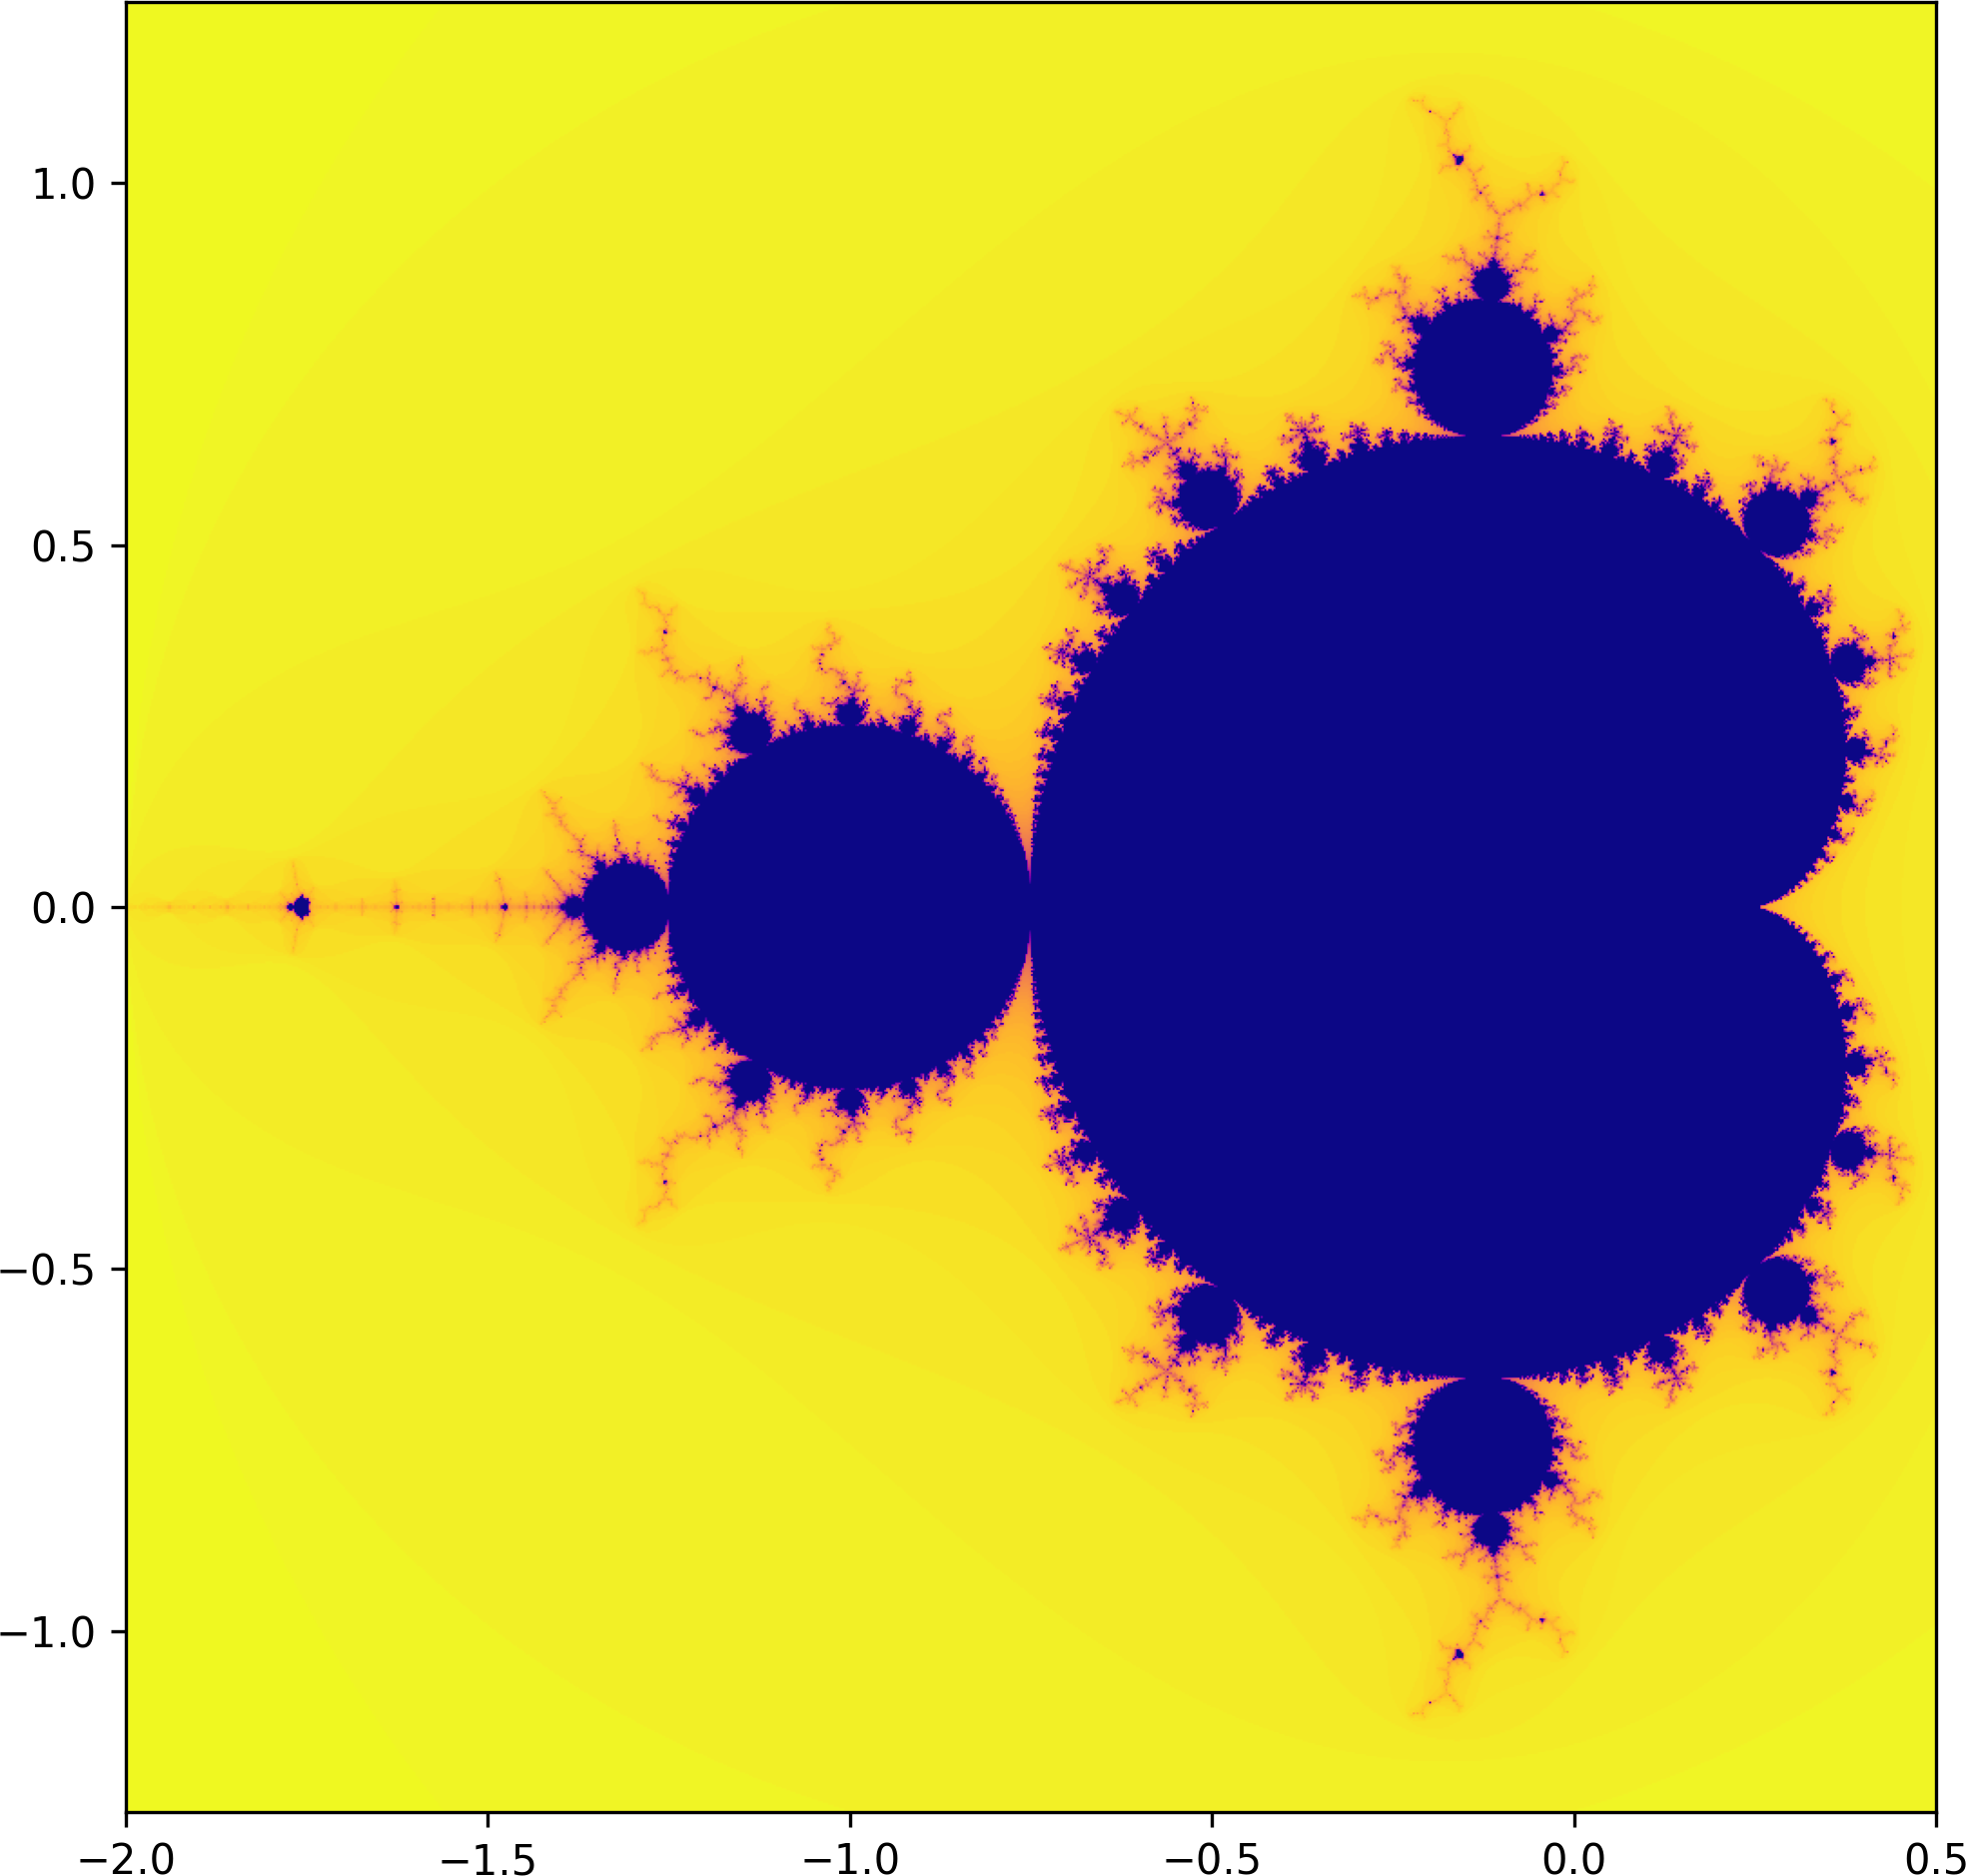
\includegraphics[width=7.25cm]{MandelbrotSet}
	\caption[Mandelbrot Set Plot]{Mandelbrot Set Plot\footnotemark}
	\label{fig:MandelbrotSet}
	\vspace{-0.75cm}
\end{wrapfigure}
\addtocounter{footnote}{-1}
\stepcounter{footnote}\footnotetext{More details on the plots in the appendix.}
\subparagraph{Contour of the Mandelbrot Set}
The Mandelbrot set is a subset of the complex plane defined as follows:
\begin{definition}[Mandelbrot Set]\label{def:MandelbrotSet}
	Let $z_0 = 0$ and $z_{n+1} = f_c(z_n)$, with $f_c(z) = z^2+c$.
	Then, the Mandelbrot set $M \subseteq \C$ is $M = \left\lbrace c \in \C \mid z_n \text{ does not diverge} \right\rbrace$.
\end{definition}

The Mandelbrot set is not a fractal itself (it has dimension 2, as it contains $\left\lbrace w \in \C \mid | w-1 | < \frac{1}{4} \right\rbrace$ \cite{3DXplorMath}, and is contained in $\C$, both having dimension 2).

It is surprising that the boundary $\partial M$ of $M$ also has Hausdorff dimension 2.
This was proved by Shishikura in 1992 \cite{Shishikura_1992}, as a consequence of $\partial M$ having a positive 2-dimensional Lebesgue measure (i.e. $\Lambda_2(\partial M) > 0$).

Despite having an integral fractional dimension, $\partial M$ is commonly considered to be a fractal (because the intergality of fractional dimension is not obvious, and the self-similarity of the set).

\subparagraph{Contour of Julia Sets}
Julia sets are also subset of the complex plane defined similarly to the Mandelbrot set:
\begin{definition}[Julia Set]\label{def:JuliaSet}
	For a complex $c \in \C$ constant:
	Let $z_0 = z$ and $z_{n+1} = f_c(z_n)$, $f_c(z) = z^2+c$ as before.
	The filled Julia set about $c$ is $K(f_c) = \left\lbrace z \in \C \mid z_n \text{ does not diverges} \right\rbrace \subseteq \C $.
	The Julia set (about $c$) $J(f_c)$ is the boundary of $K(f_c)$ ($J(f_c) \subseteq \C$).
\end{definition}

The dimension of $J(f_c)$ will of course depend on $c$.
It is considered as a fractal even when the dimension is an integer.
For some values of $c$, dimension of $J(f_c)$ is well known:

\vspace{0.2cm}
\begin{tabular}{l l l}\label{table:JuliaSetDimensions}
%	$c$ & $\dim_H(J(f_c))$ & Popular Name \\
%	\hline
	$c = 0$             & $\dim_H(J(f_c)) = 1$            & "Circle"\\
	$c = \frac{1}{4}$   & $\dim_H(J(f_c)) \approx 1.0812$ & \\
	$c = i$             & $\dim_H(J(f_c)) \approx 1.2$    & "Dendrite" \\
	$c = -1$            & $\dim_H(J(f_c)) \approx 1.2683$ & \\
	$c = -0.123+0.745i$ & $\dim_H(J(f_c)) \approx 1.3934$ & "Douady rabbit" \\
\end{tabular}
\vspace{0.3cm}

The Mandelbrot set and Julia sets are very closely related.
In fact, Shishikura proved \cite{Shishikura_1992} that when $c$ is on $\partial M$, then the Julia set $J(f_c)$ associated to it has (Hausdorff) dimension 2.
Moreover, Heinemann and Stratmann have shown \cite{Heinemann_Stratmann_1998} that when the quadratic $f_c$ is parametrized with $c$ near the boundary of the Mandelbrot set $M$, the Hausdorff dimension of $J(f_c)$ is arbitrarily close to 2.

\begin{figure}[h]
	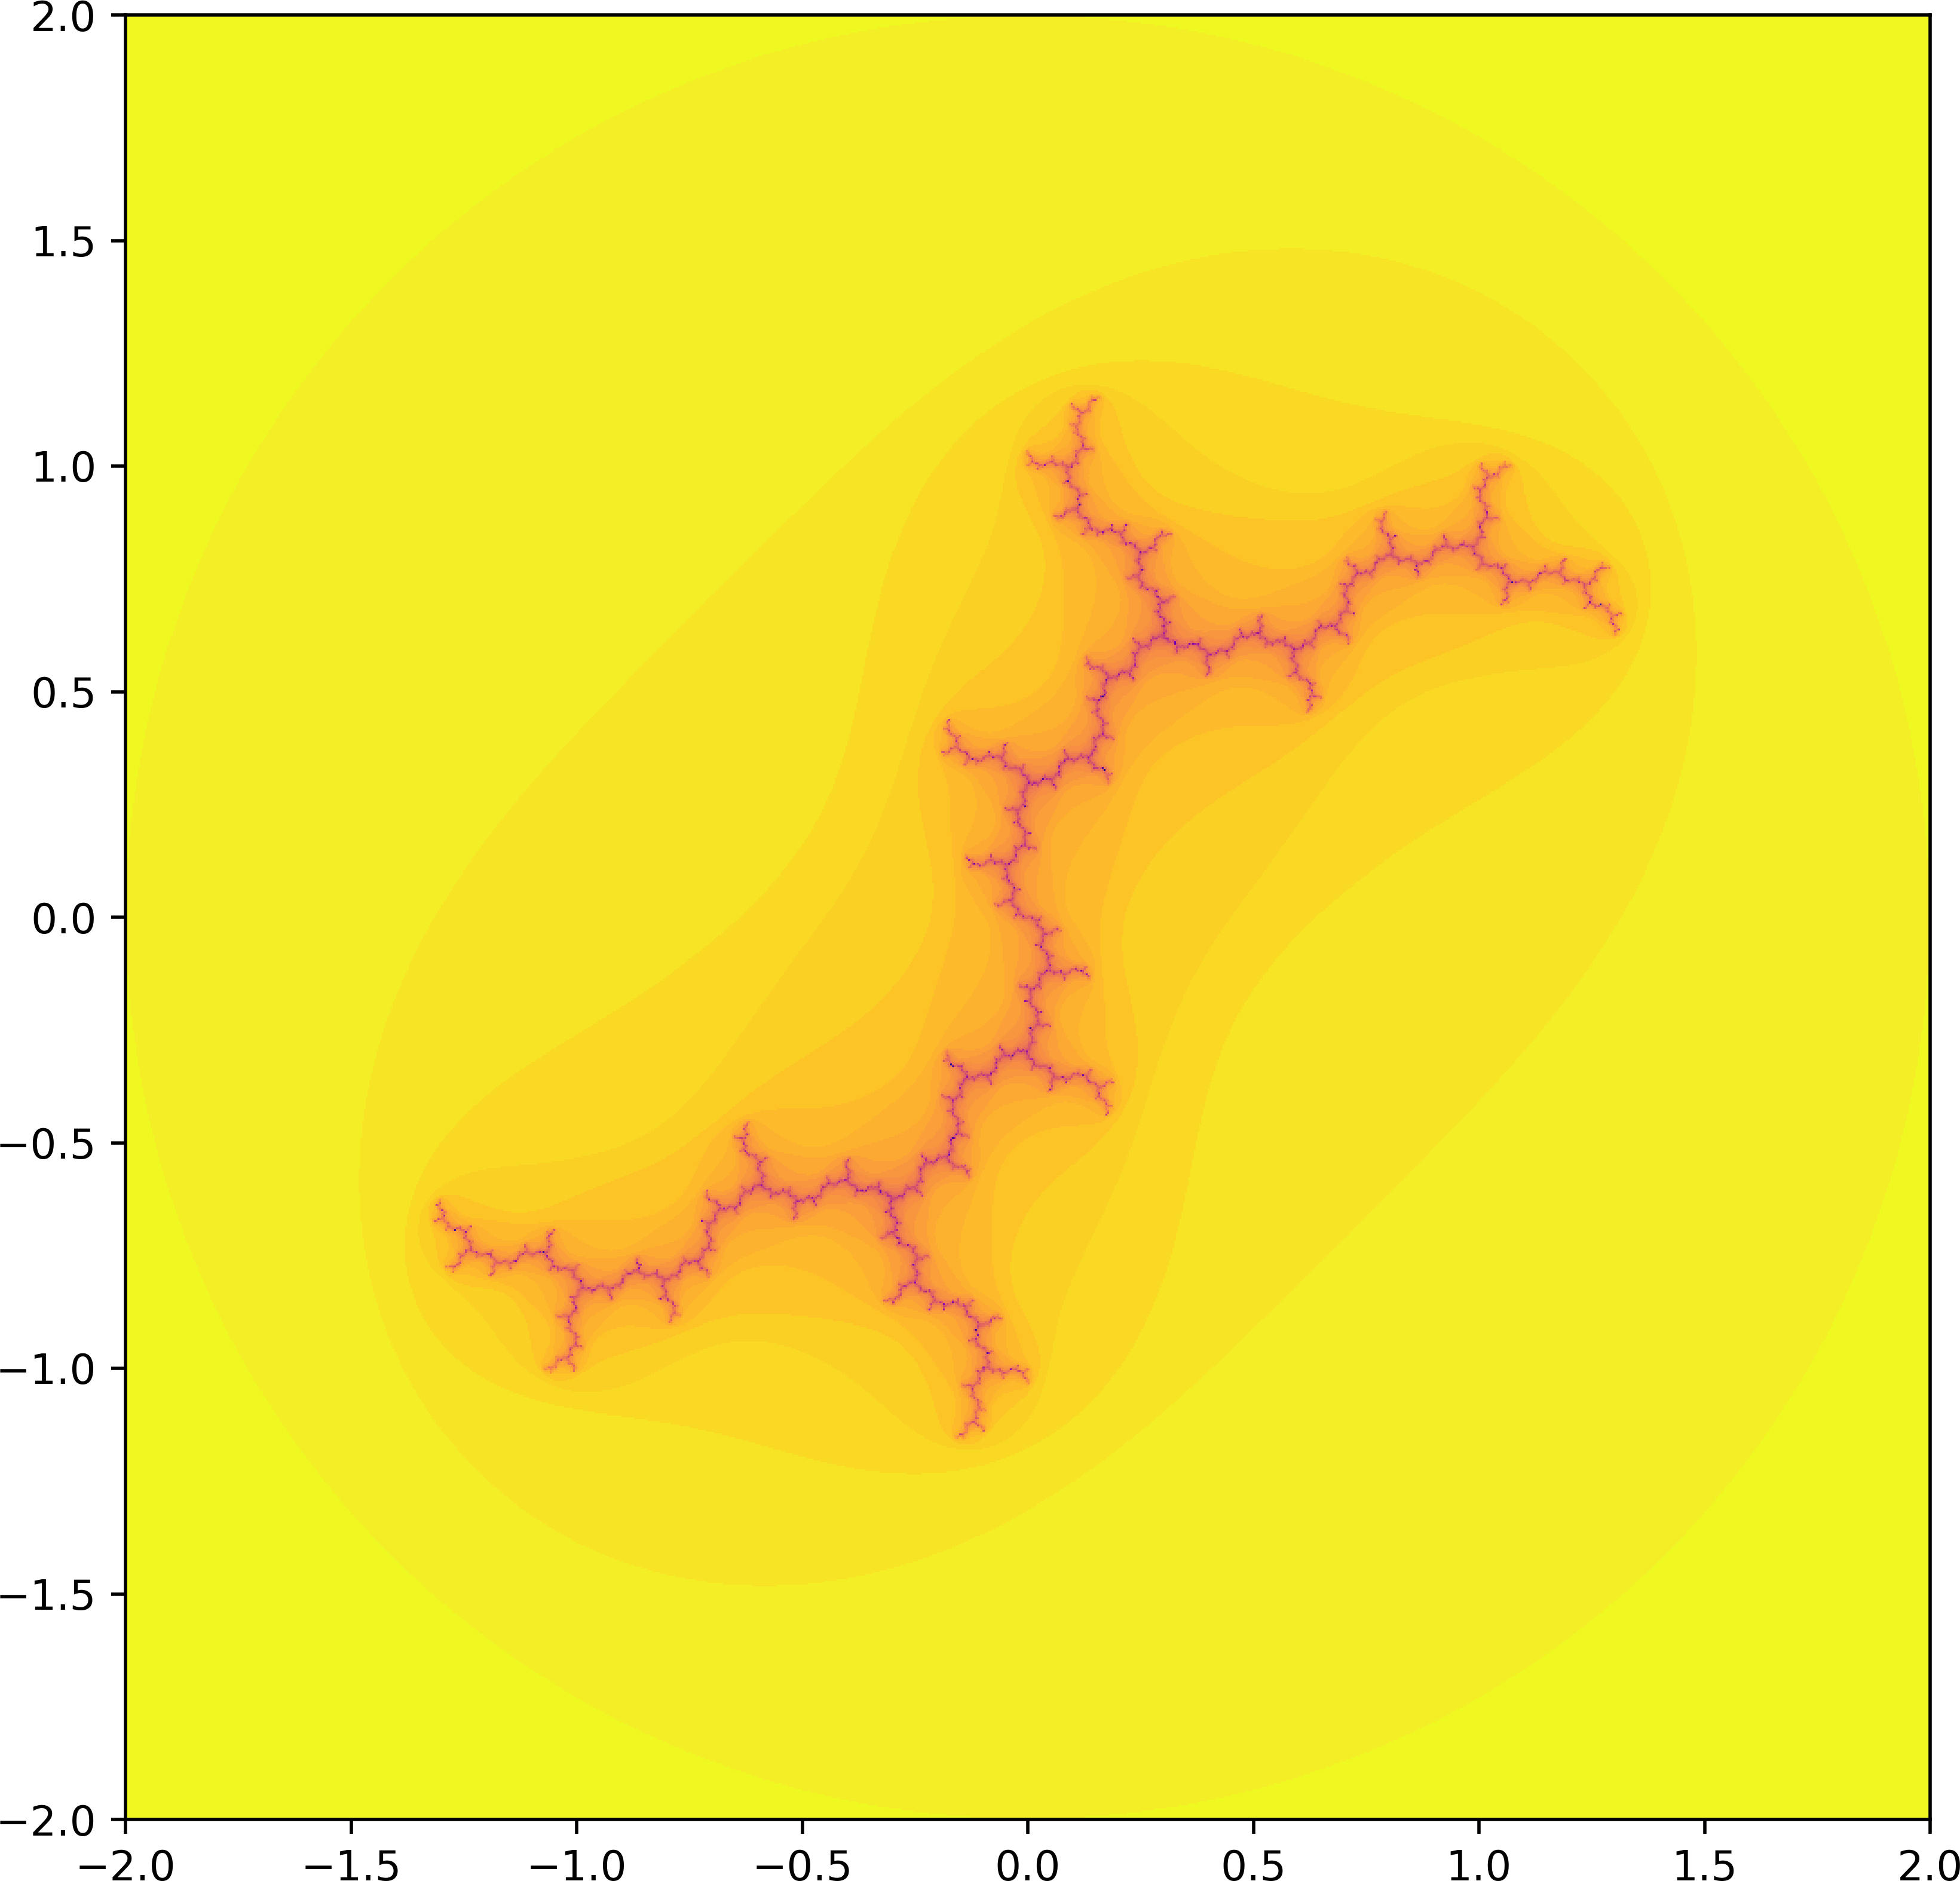
\includegraphics[width=5.4cm]{dendrite}
	\hspace{0.15cm}
	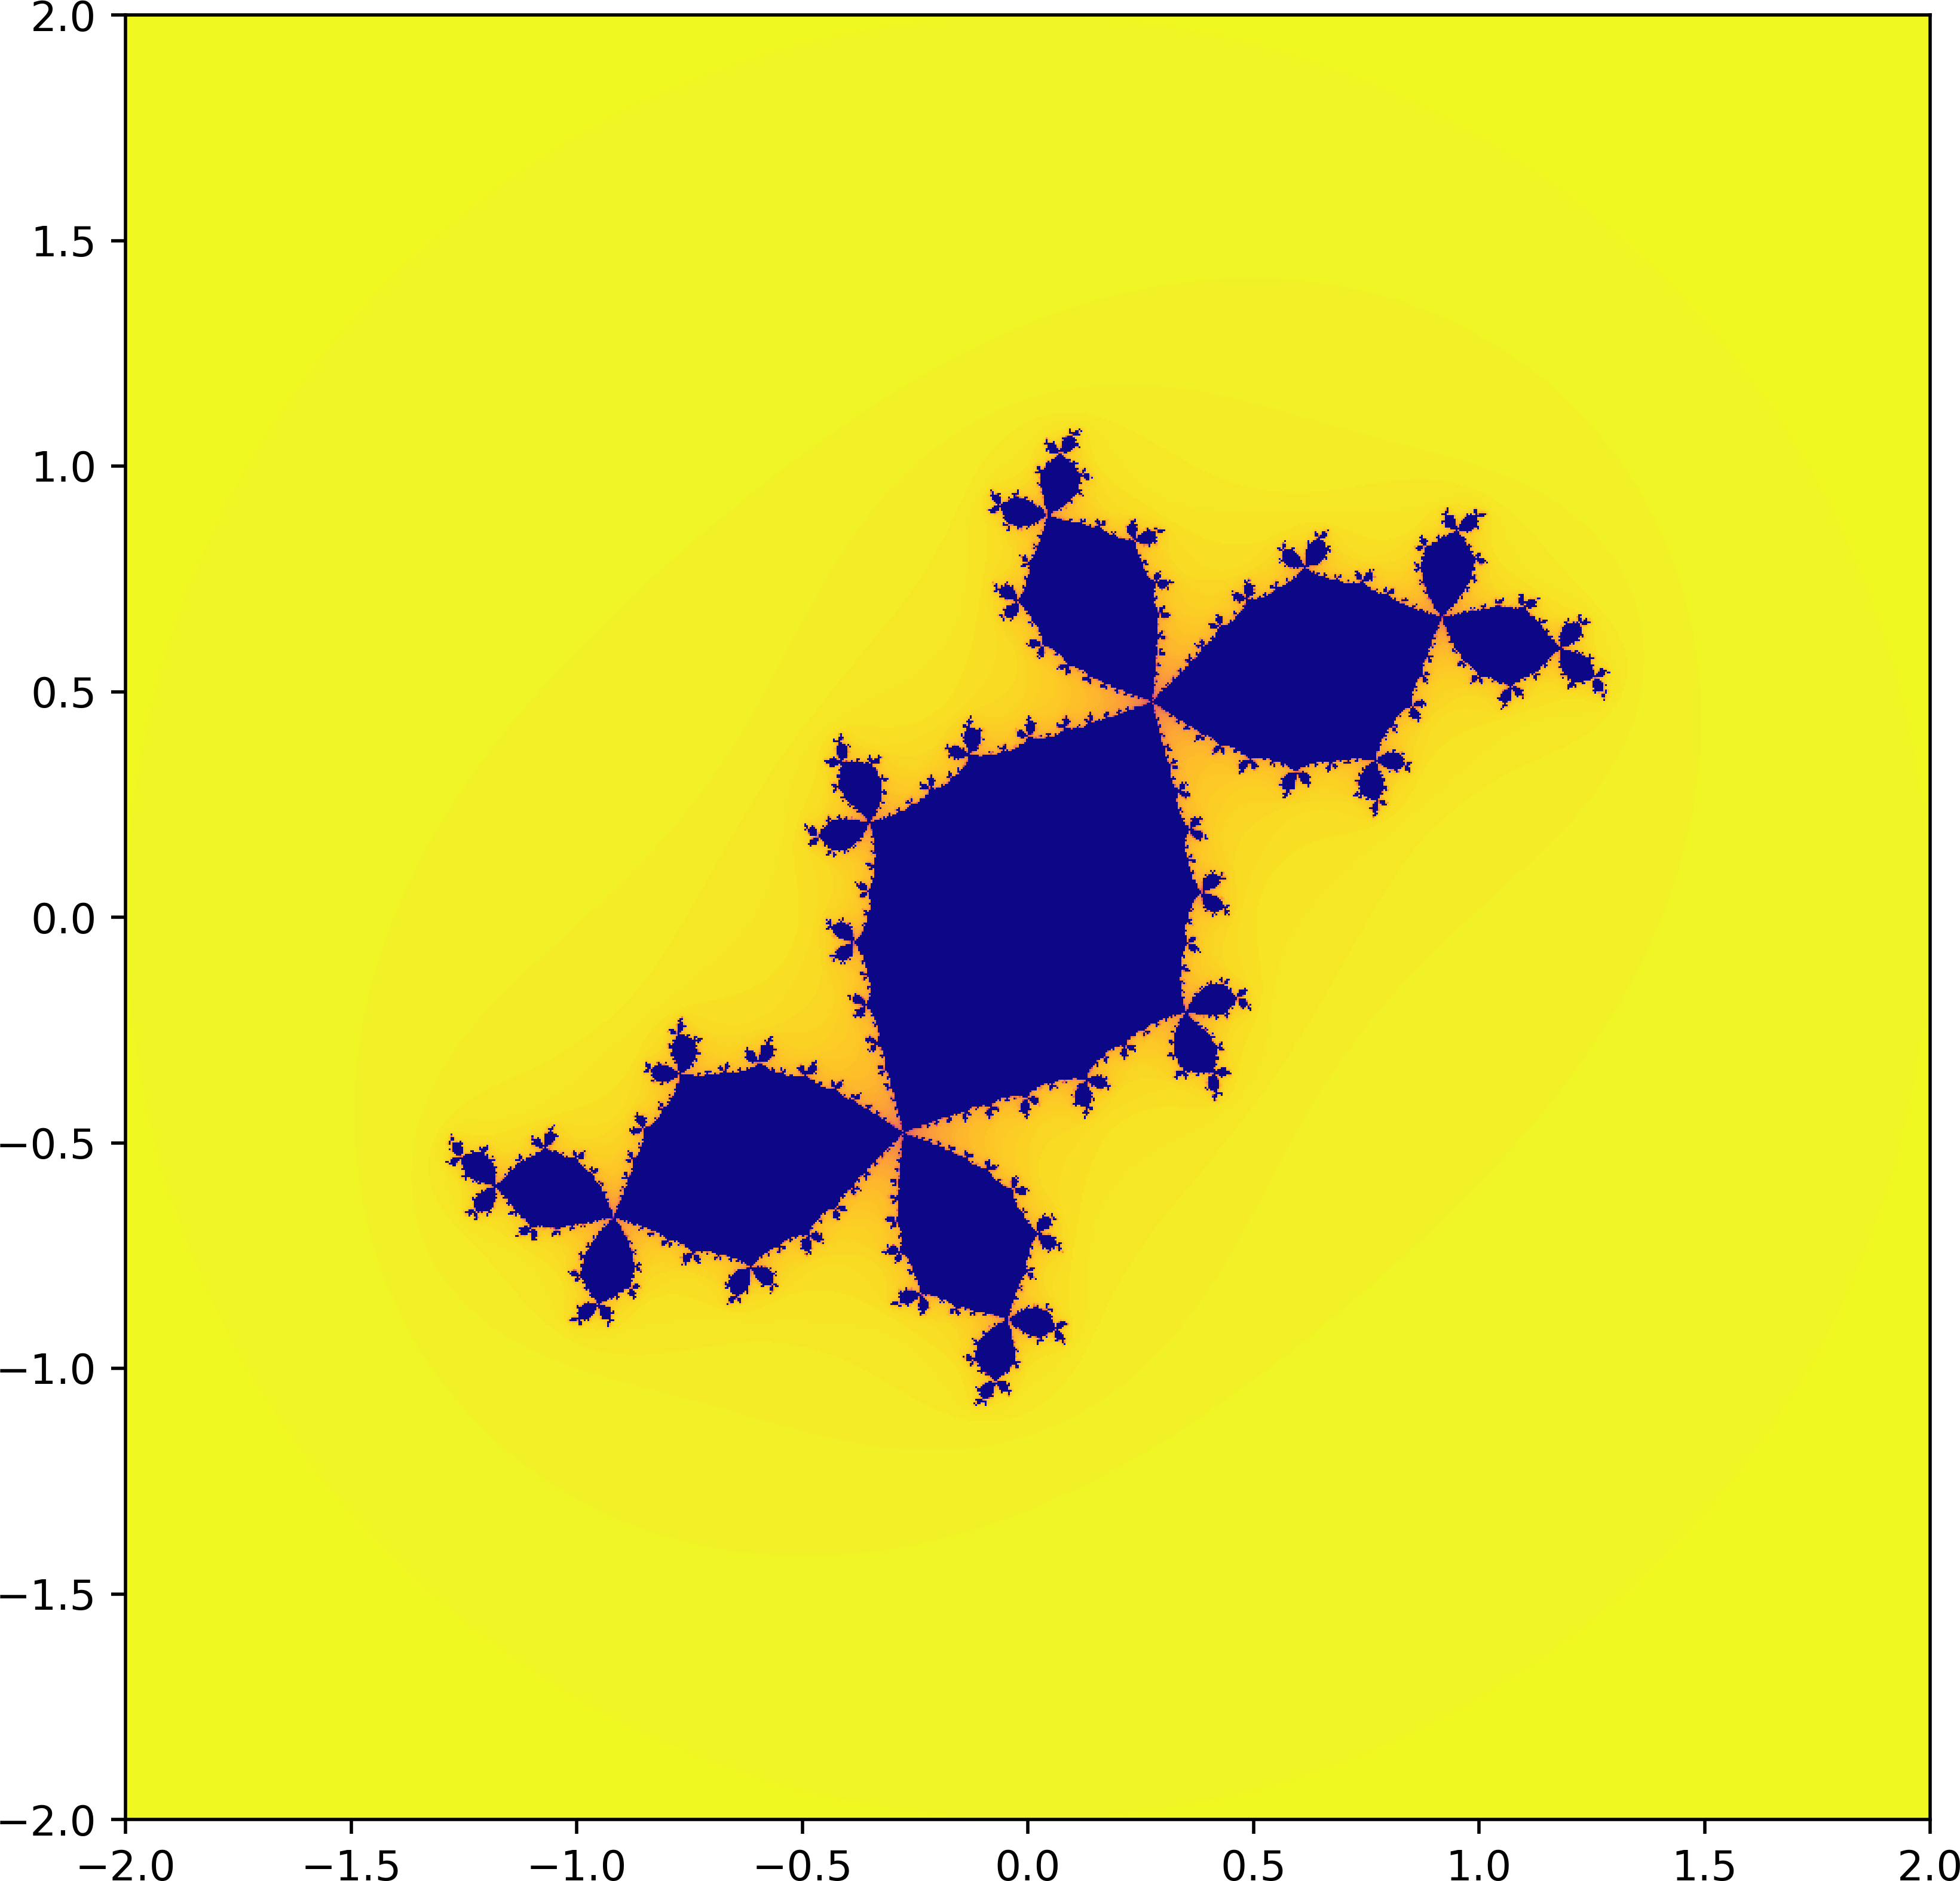
\includegraphics[width=5.4cm]{DouadyRabbit}
	\hspace{0.15cm}
	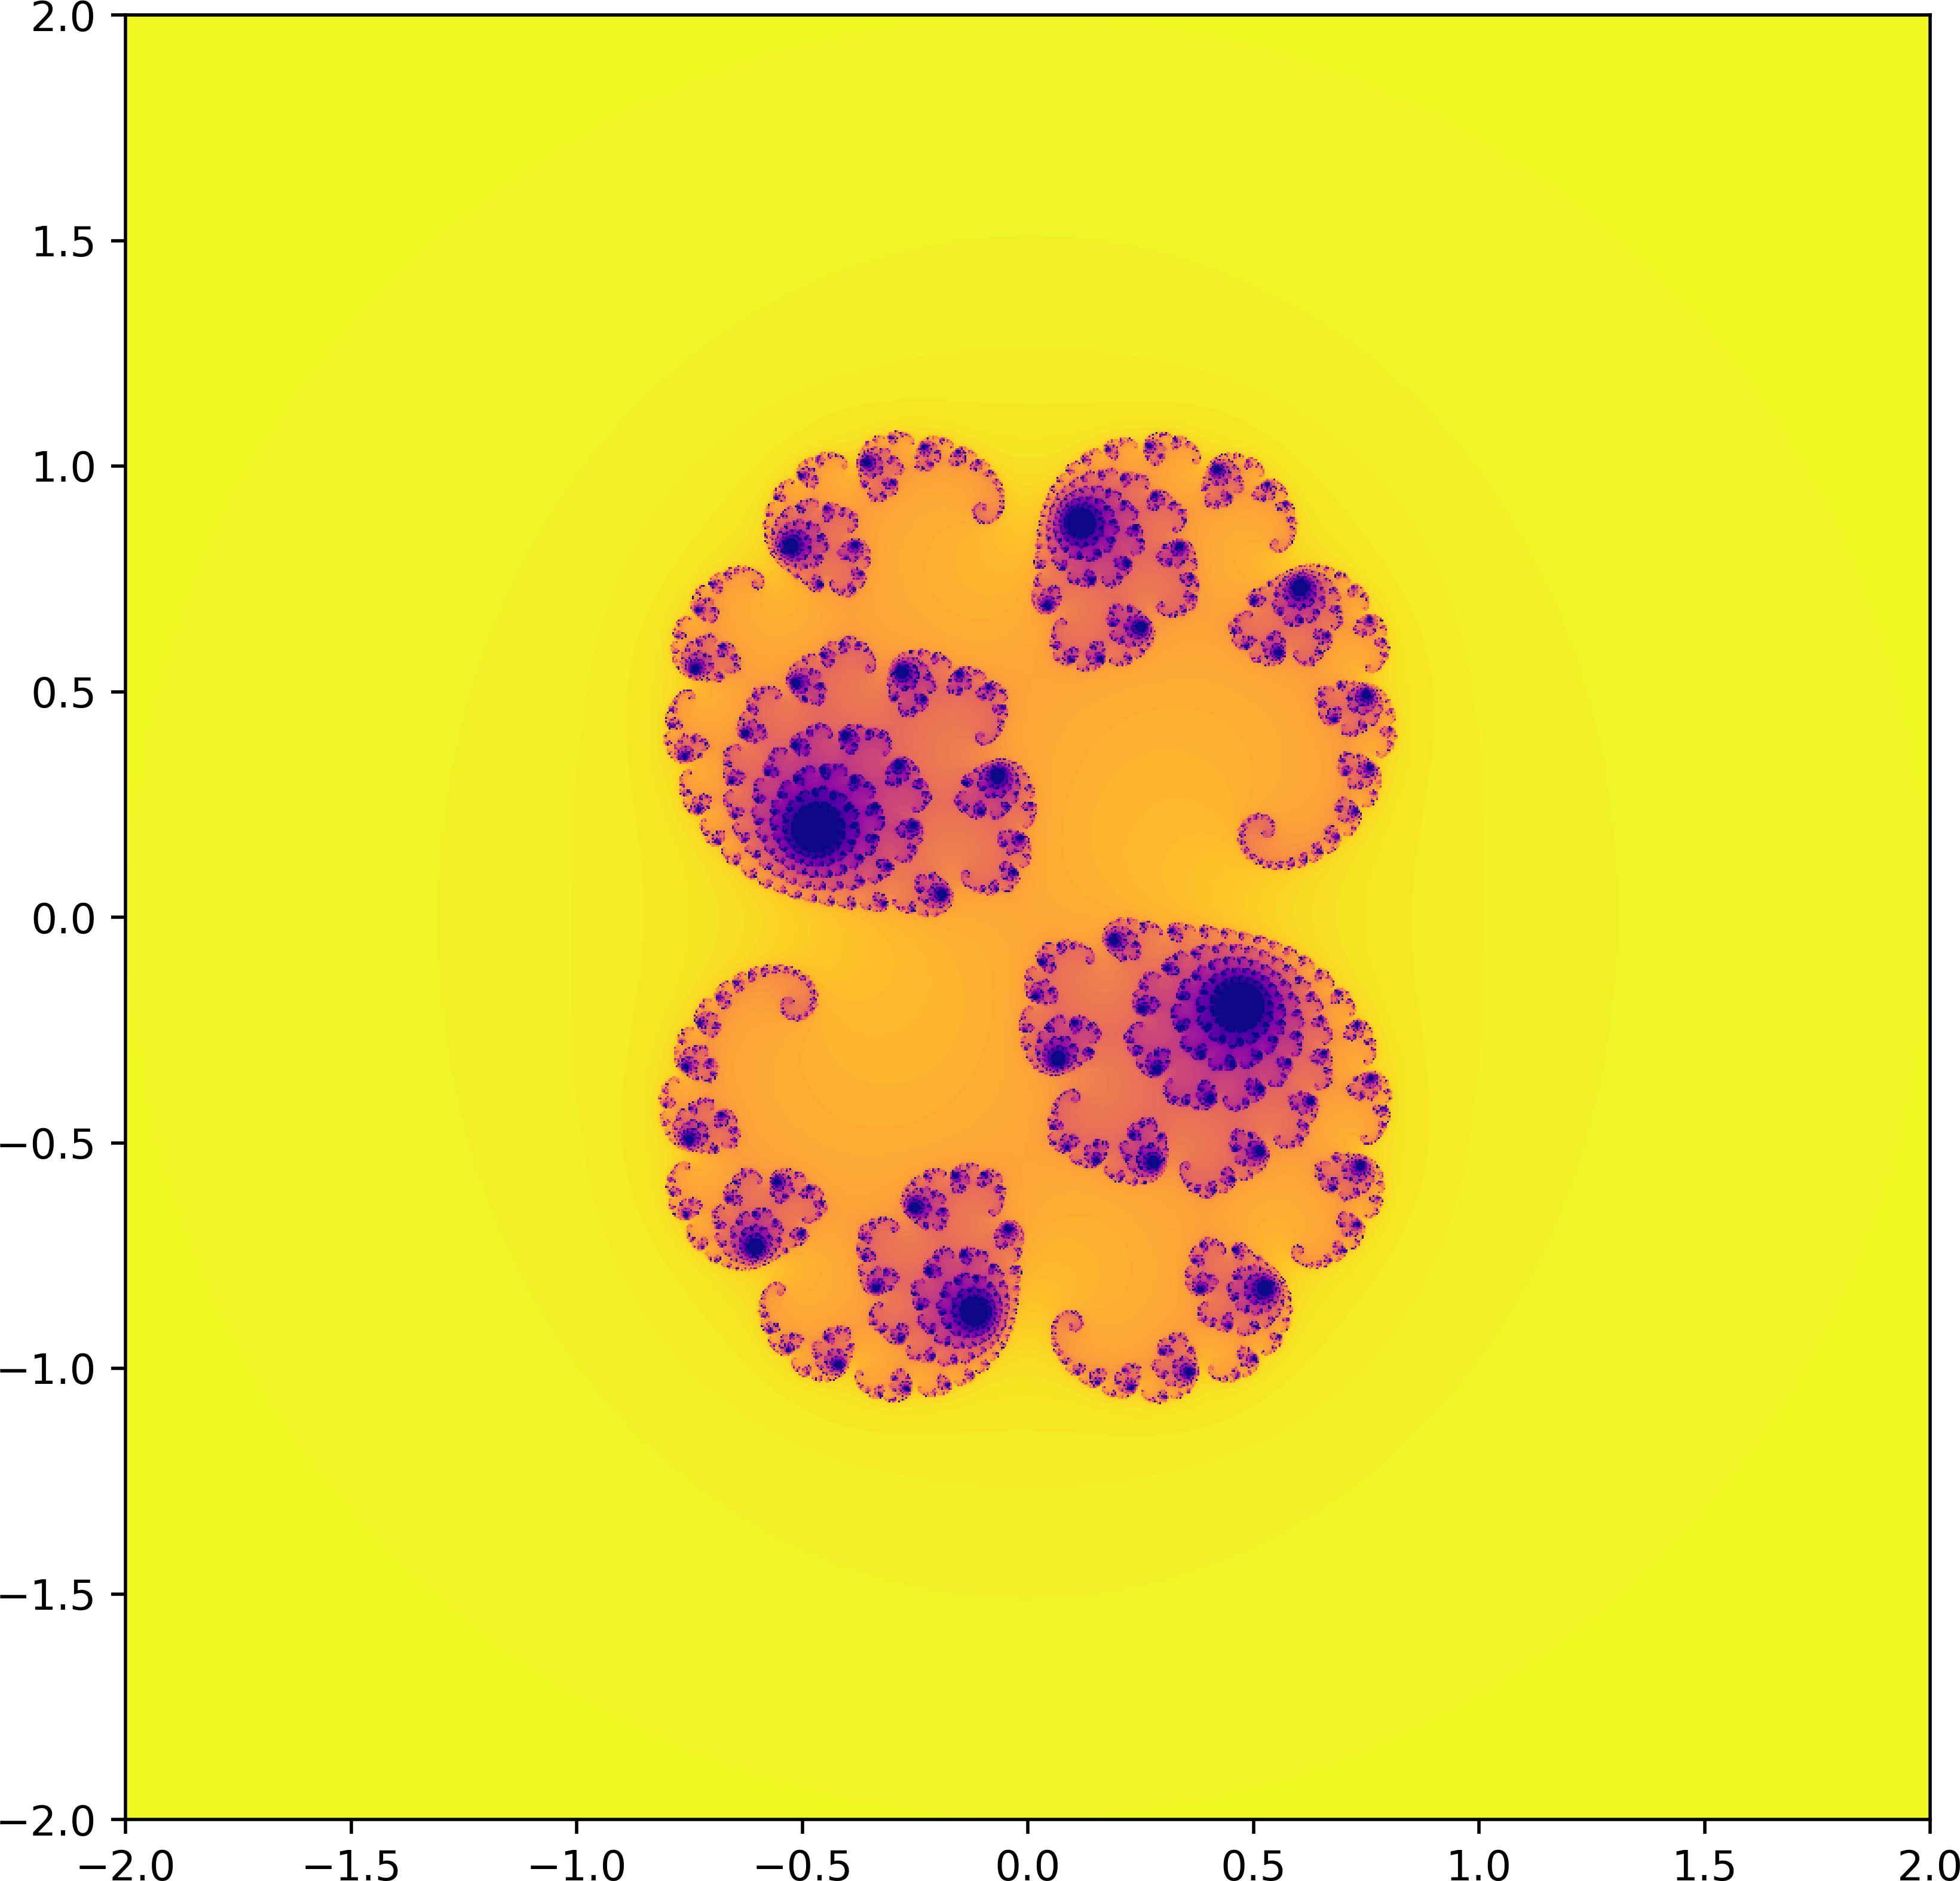
\includegraphics[width=5.4cm]{JuliaSet_0_285+0_01i}
	\centering
	\captionsetup{justification=centering}
	\caption[Julia sets examples]{Popular Julia Set Plots \newline (left to right: "Dendrite"\footnotemark; "Douady rabbit"\footnotemark; other typical Julia set\footnotemark)}
	\label{fig:JuliaSets}
\end{figure}
\addtocounter{footnote}{-3}
\stepcounter{footnote}\footnotetext{$c = i$}
\stepcounter{footnote}\footnotetext{$c = -0.123+0.745i$}
\stepcounter{footnote}\footnotetext{$c = 0.285+0.01i$}



\vspace{-0.5cm}
\begin{wrapfigure}{r}{5cm}
	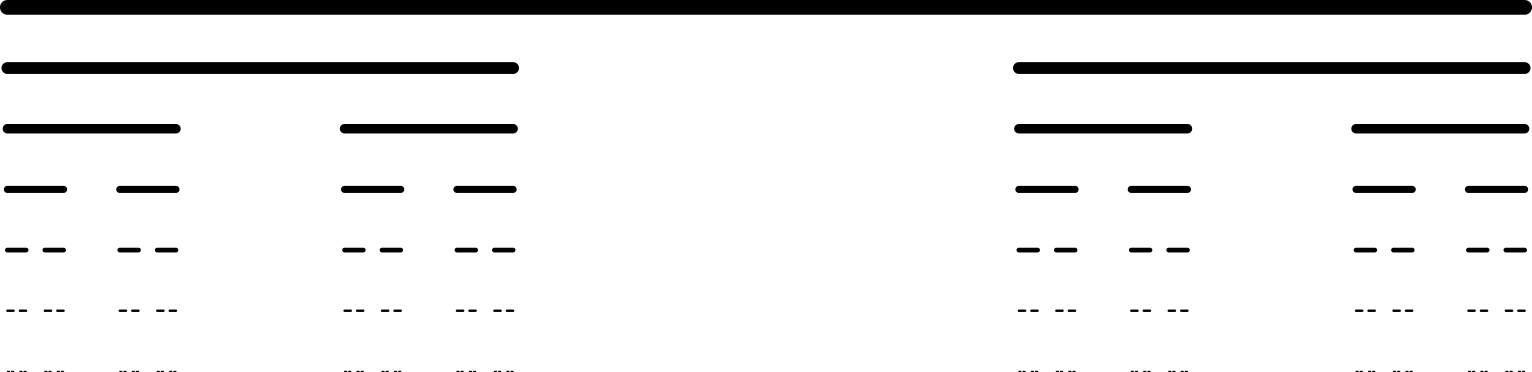
\includegraphics[width=5cm]{CantorSet}
	\centering
	\captionsetup{justification=centering}
	\caption{Cantor Set (first 6 iterations)}
	\label{fig:CantorSet}
	\vspace{-1.5cm}
\end{wrapfigure}
\paragraph{Cantor Set}
The (middle third) Cantor set $C \subseteq \left[ 0,1 \right] $ is constructed via the following informal definition:
\begin{itemize}
	\item Start with $C_0 = \left[ 0,1 \right]$
	\item Generate iteratively $C_n = \frac{C_{n-1}}{3} + \frac{2 + C_{n-1}}{3}$
	\item Take the limit $C = \lim_{n \to \infty} C_n$
\end{itemize}

The Cantor set satisfies $C = \frac{C}{3} + \frac{2 + C}{3}$, so rescaling by $\frac{1}{3}$, it contains two copies of itself.
So the intuitive Hausdorff dimension for the Cantor set is $\dim_H(C) = \frac{\log(2)}{\log(3)} \approx 0.631$.
This can be proved rigorously (see \cite[p. 34-35, ex. 2.7]{Falconer_1990}.

Another equivalent definition for the cantor set $C$ is "points in $\left[ 0,1 \right]$ with extension in base 3 composed of 0 and 2 only".
That is:
$$
C = \left\lbrace x \in \left[ 0,1 \right] \mid x = \sum_{k=1}^{\infty} x_k 3^{-k}, \ \ x_k \in \{0,2\} \ \forall k \right\rbrace
$$
From this definition, it is straightforward that the Cantor set is totally disconnected.
In fact, fractals with Hausdorff dimension smaller than 1 are totally disconnected (\cite[p. 33, prop. 2.5]{Falconer_1990}).

\begin{wrapfigure}{r}{5cm}
	\vspace{-0.5cm}
	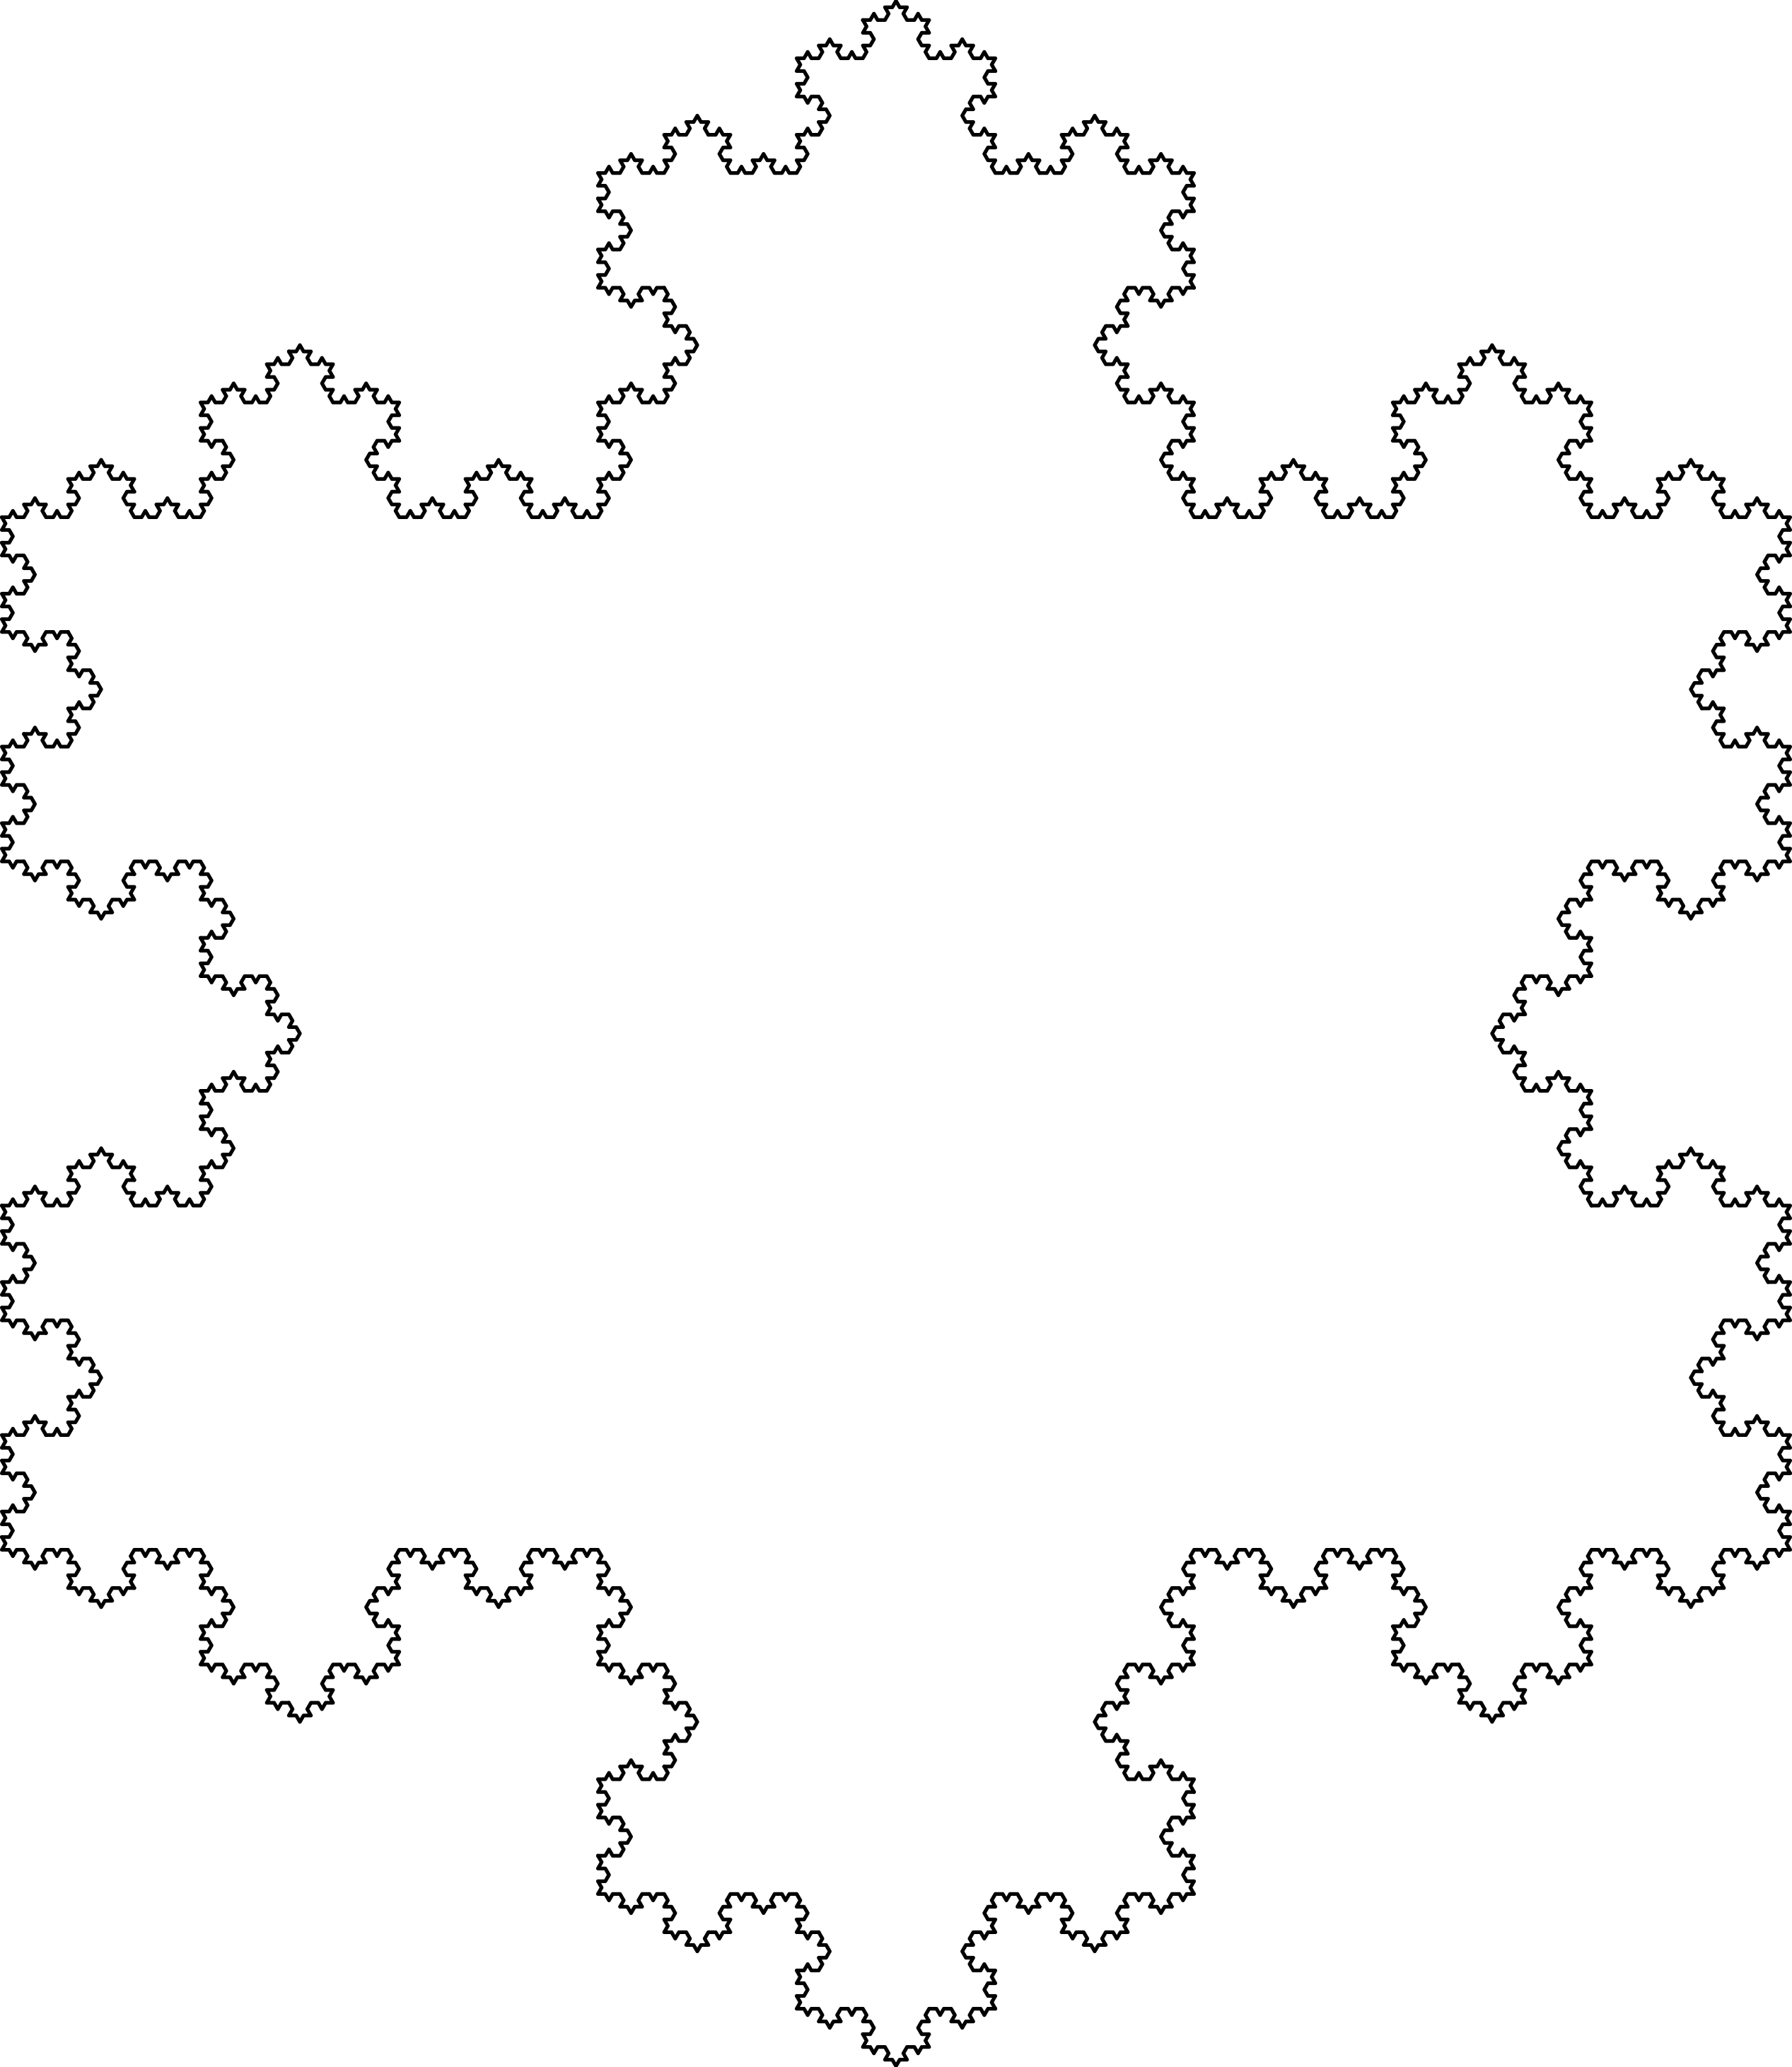
\includegraphics[width=5cm]{KochSnowflake}
	\centering
	\captionsetup{justification=centering}
	\caption{Koch Snowflake Curve Plot (5 iterations)}
	\label{fig:KochSnowflake}
\end{wrapfigure}
\paragraph{Koch Snowflake}
The Koch Snowflake is an example of a fractal curve.
Fractal curves are obtained by applying the same transformation recursively to each segment of the previous iteration of the curve.
Their fractional dimension is in the interval $\left[ 1,2 \right]$ (or in $\left[ 1,3 \right]$ if the curve evolves in a three dimensional space).

The Koch snowflake is obtained after replacing each edge of an equilateral triangle by a Koch curve with the triangle edge as initial segment.

Now, the Koch curve is defined recursively as follows:
$K_n$ is the curve at iteration $n$, with segments $K_n^1, \dots K_n^m$.
For each $i \in \llbracket 1,m \rrbracket$, split $K_n^i$ into 3 equal length segments, and replace the middle one with two new ones as on this diagram:\vspace{0.2cm}\\
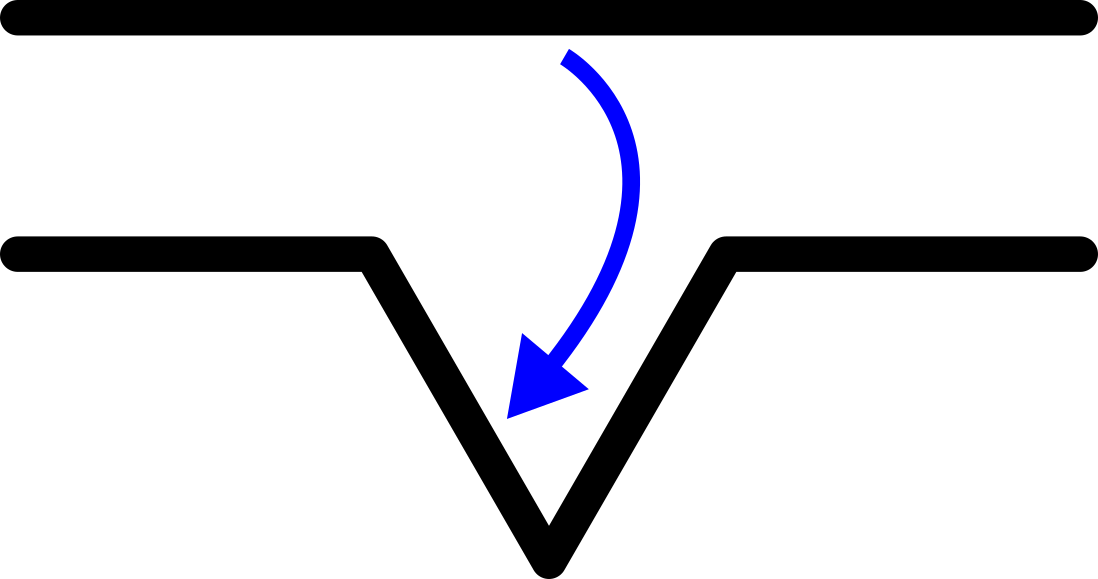
\includegraphics[width=4.5cm]{KochStep}\vspace{0.2cm}\\
Merging back all segment gives $K_{n+1}$.

The Koch curve starting form a segment $[a,b]$ is the limit curve $K = \lim_{n \to \infty} K_n$ with $K_0 = [a,b]$.

At each level, the Koch curve is scaled by $\nicefrac{1}{3}$, and $4$ copies are created.
Thus, the intuitive Hausdorff dimension for the Koch curve (which is also the dimension of the Koch snowflake) is $\dim_H(K) = \frac{\log(4)}{\log(3)} \approx 1.262$.
This can be proved rigorously using similar techniques as in \cite[p. 34-35, ex. 2.7]{Falconer_1990}.

\begin{wrapfigure}{r}{5cm}
	\vspace{-0.75cm}
	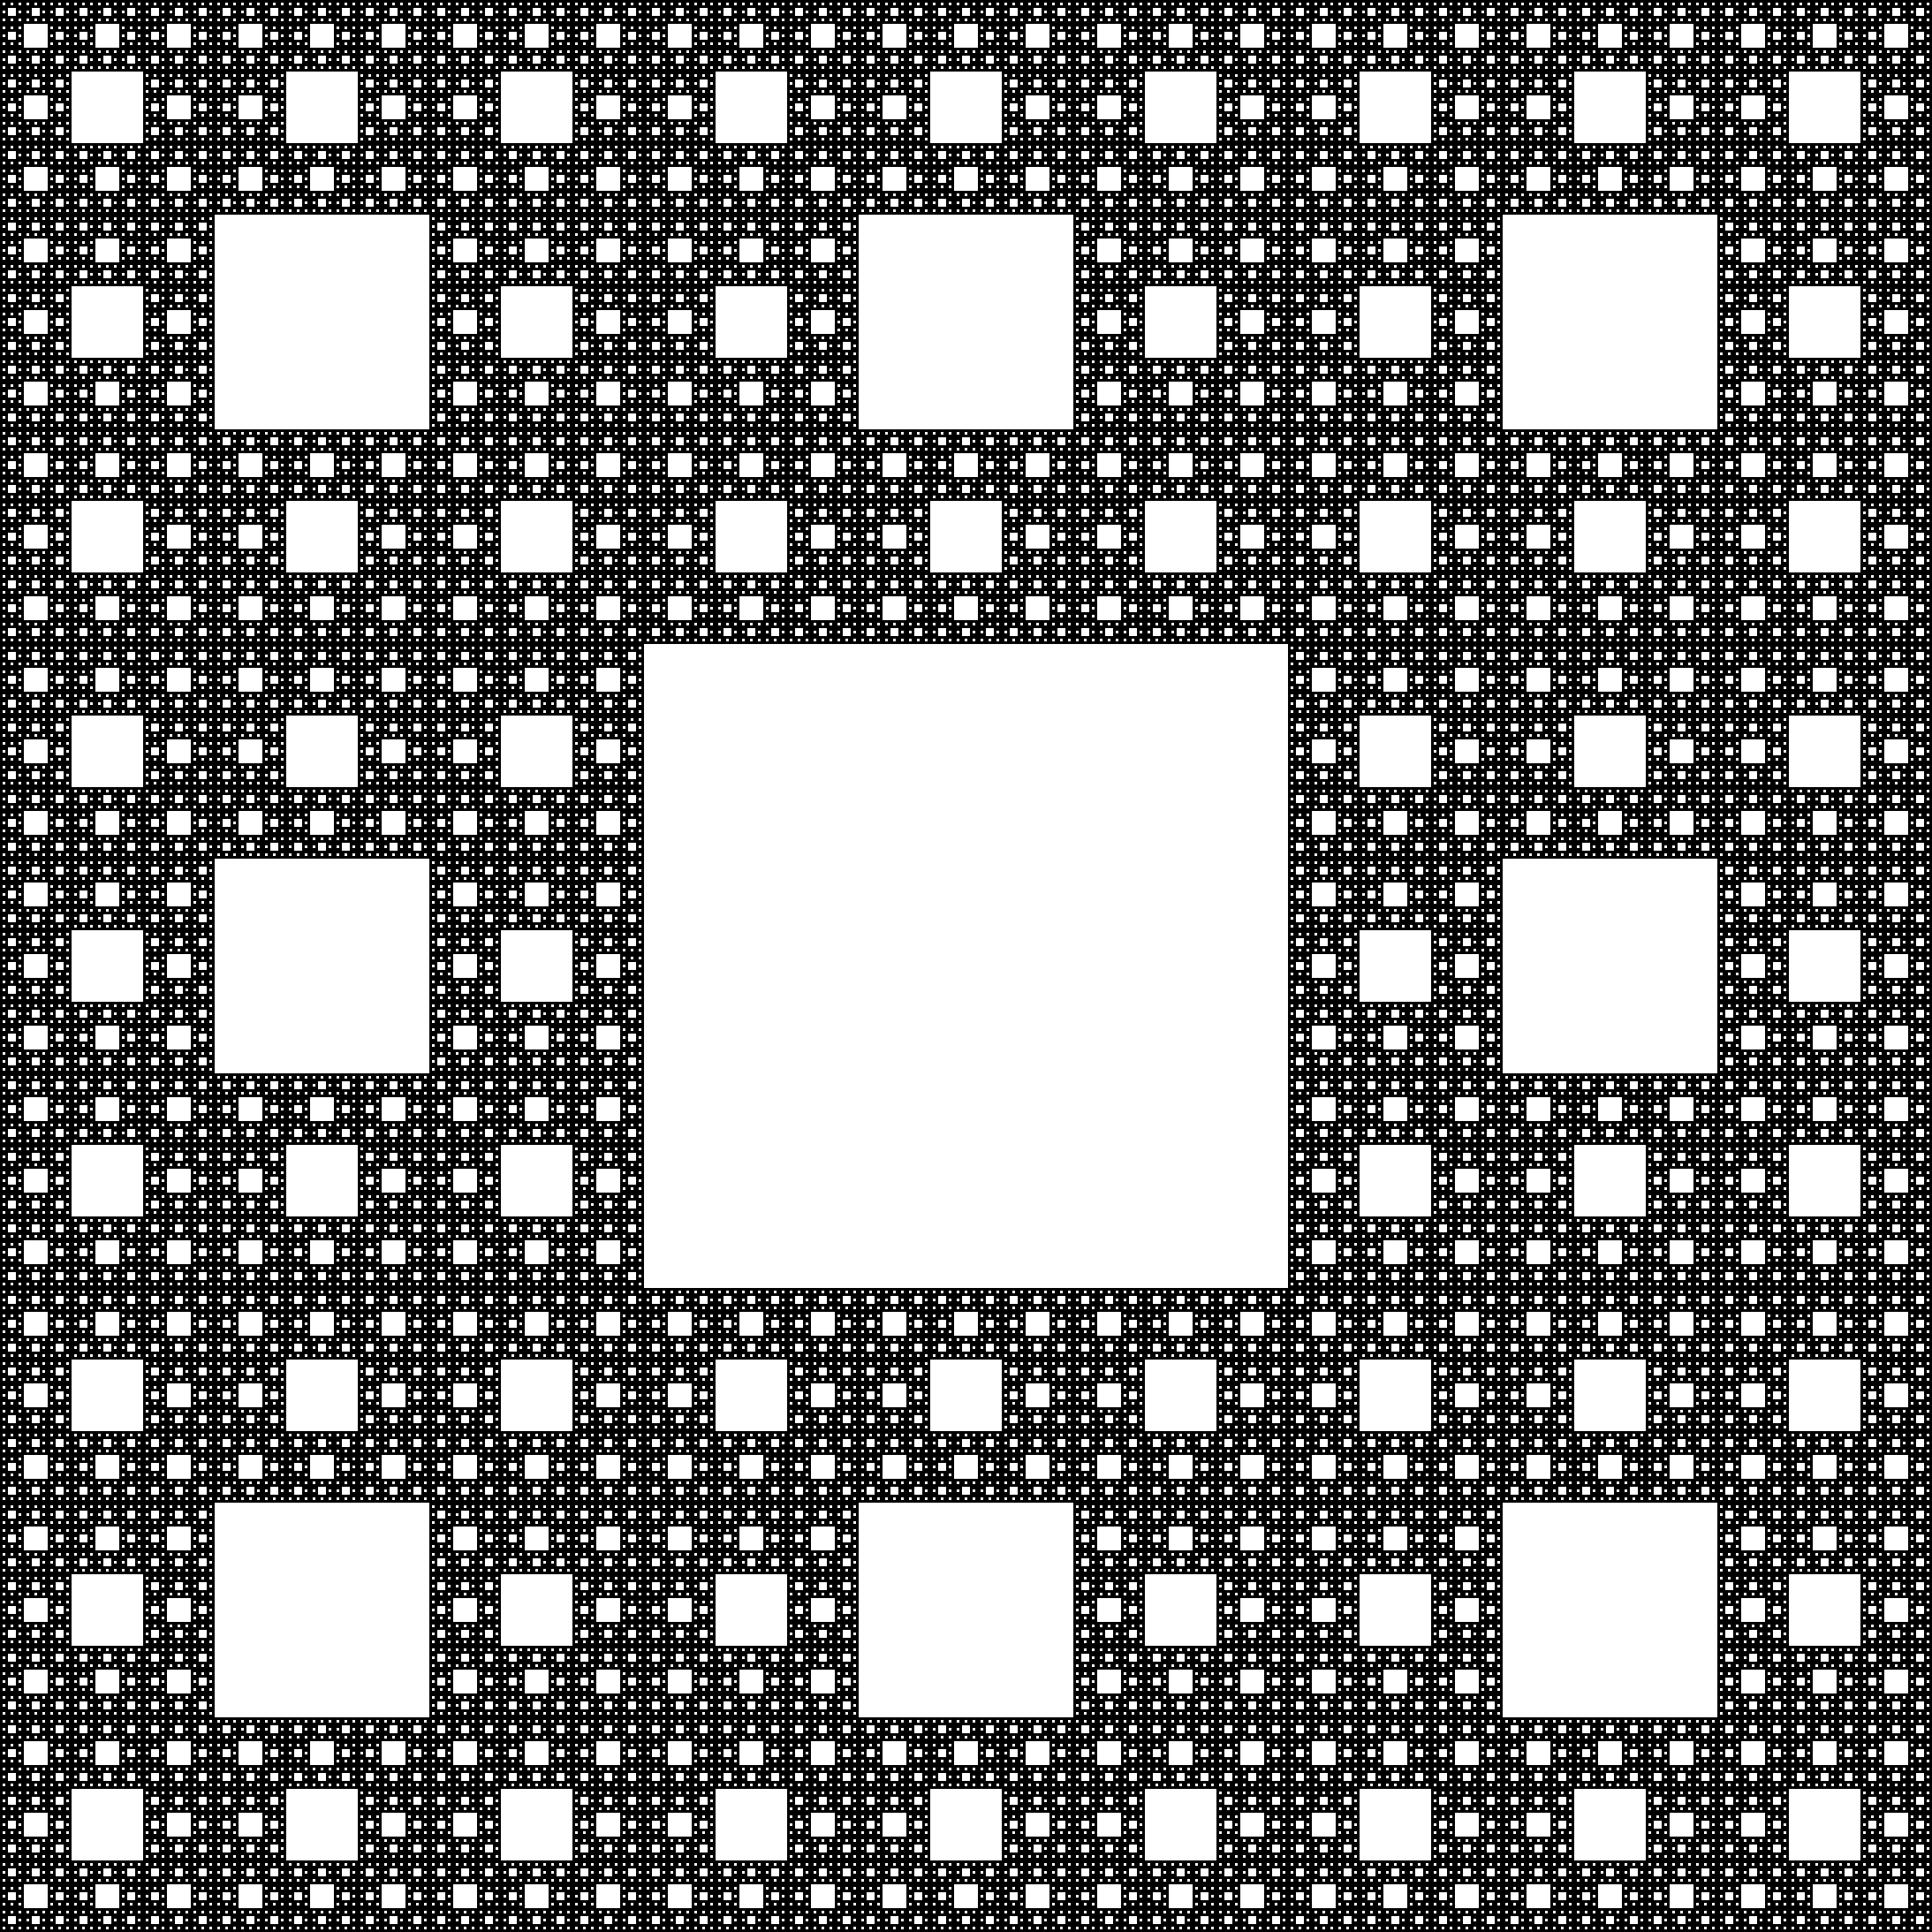
\includegraphics[width=6cm]{SierpinskiCarpet}
	\centering
	\captionsetup{justification=centering}
	\caption{Sierpinski Carpet (6 steps)}
	\label{fig:SierpinskiCarpet}
	\vspace{-3cm}
\end{wrapfigure}
\paragraph{Sierpiński Carpet}
Sierpiński carpet is a fractal constructed recursively by removing parts of its initial set.

The construction starts from a (filled) square.
Then, at each step, split every square into 9 sub-square as follows:\\
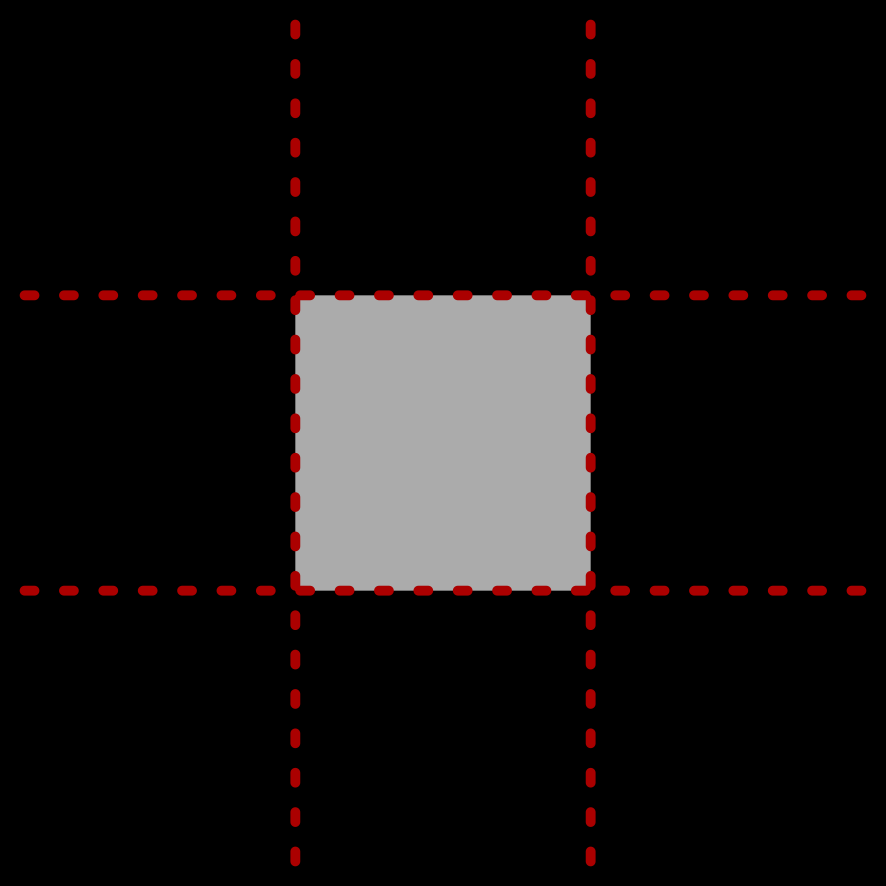
\includegraphics[width=4cm]{SierpinskiCarpetStep}\\
Remove the central square, and repeat the operation on the remaining 8 squares.

Note that this can be seen as a version of the Cantor set starting in 2 dimensions.

The figure is made of $8$ copies of itself, scaled by a factor of $\nicefrac{1}{3}$.
Therefore, the intuitive Hausdorff dimension for this set is $\dim_H(K) = \frac{\log(8)}{\log(3)} \approx 1.893$.
Again, this can be proved rigorously using similar techniques as in \cite[p. 34-35, ex. 2.7]{Falconer_1990}.


\subsubsection{Real Life Fractals}
Fractals are more than mathematical constructions, in fact self-similarity structures also occur in nature.
The limit is never reached, because of the physical constraints, but we can view them as natural approximations of fractals.
This gives a good motivation for studying fractals in a mathematical context.

\paragraph{Plants}
Some plants (not even genetically modified) have self-similarity patterns, and may therefore be considered as fractals.

\subparagraph{Ferns}
Perhaps the most obvious and popular natural fractal: Ferns leaves.
The leaves are self-similar, with varying pattern across variety of ferns.

\subparagraph{Cauliflower}
A less obvious example: Cauliflowers' surface is a fractal.
In fact, since each branch splits into about 13 branches, each about 3 times shorter, the approximate dimension of a Cauliflower's surface is $\log_3(13) \approx 2.335$.

\begin{figure}[!h]
	\centering
	\begin{subfigure}{.49\textwidth}
		\includegraphics[height=3cm]{Fern}
		\centering
		\captionsetup{justification=centering}
		\caption{Fern Leave}
		\label{fig:fern}
	\end{subfigure}
	\begin{subfigure}{.49\textwidth}
		\includegraphics[height=3cm]{Cauliflower}
		\centering
		\captionsetup{justification=centering}
		\caption{Cauliflower}
		\label{fig:cauliflower}
	\end{subfigure}
	\caption{Plant Fractals}
	\label{fig:plantsFractals}
\end{figure}

\paragraph{Coastline of Islands}
When trying to measure the length of coastlines, scientists realized that the more precise their attempt was, the higher was the value of the length found.
In fact, this makes sense: the approximation of a curve with shorter segments will capture more of the smaller curve details, resulting in a longer length.
The approximate length found could be made really large after approximating using smaller and smaller segments (until physical boundary are reached).
This yields the fact that the coastline is a fractal with dimension greater than one.

Using electronic maps, we try to estimate the fractal dimension of the coastlines for the UK islands, Iceland and Madagascar.
More details on the calculations techniques used are given in the appendix (see \ref{appendix:coastlines}).
The (approximate) coastline dimension for UK, Iceland, and Madagascar are respectively $1.24$, $1.25$, and $1.06$.

The coastlines of the UK and Iceland are much more irregular than the one of Madagascar.
The approximate values found for coastlines dimensions therefore make sense.

	% !TeX spellcheck = en_GB
\section{Percolation Fractals}
Percolated fractals will be the main object we intend to study.

We will begin with the definition of the percolation process in the 2D case, as it will be our main interest (it is also the most intuitive case, as easy to picture).

\subsection{Plain Percolation}
%def
\subsection{Recursive Percolation}
%def
\subsection{Extension to other dimensions}
\paragraph{Extension to 3D}
\paragraph{Extension to $N$-D}
\paragraph{Restriction to 1D}

\subsection{Dimensionality}
\paragraph{Expected dimension}

\subsection{Blob}
To have a better understanding, we begin by studying the central "blob" of the fractal.
\paragraph{Definition}
\paragraph{Algorithm}
\subsubsection{Manhattan (step) distance}
%plots and plots comments
\subsubsection{Euclidean distance}
%plots and plots comments
\subsubsection{Area}
%plots and plots comments
\subsubsection{Volume}
%plots and plots comments




	% !TeX spellcheck = en_GB
\begin{wrapfigure}{r}{8.7cm}
	\vspace{-0.75cm}
	\begin{subfigure}{4.3cm}
		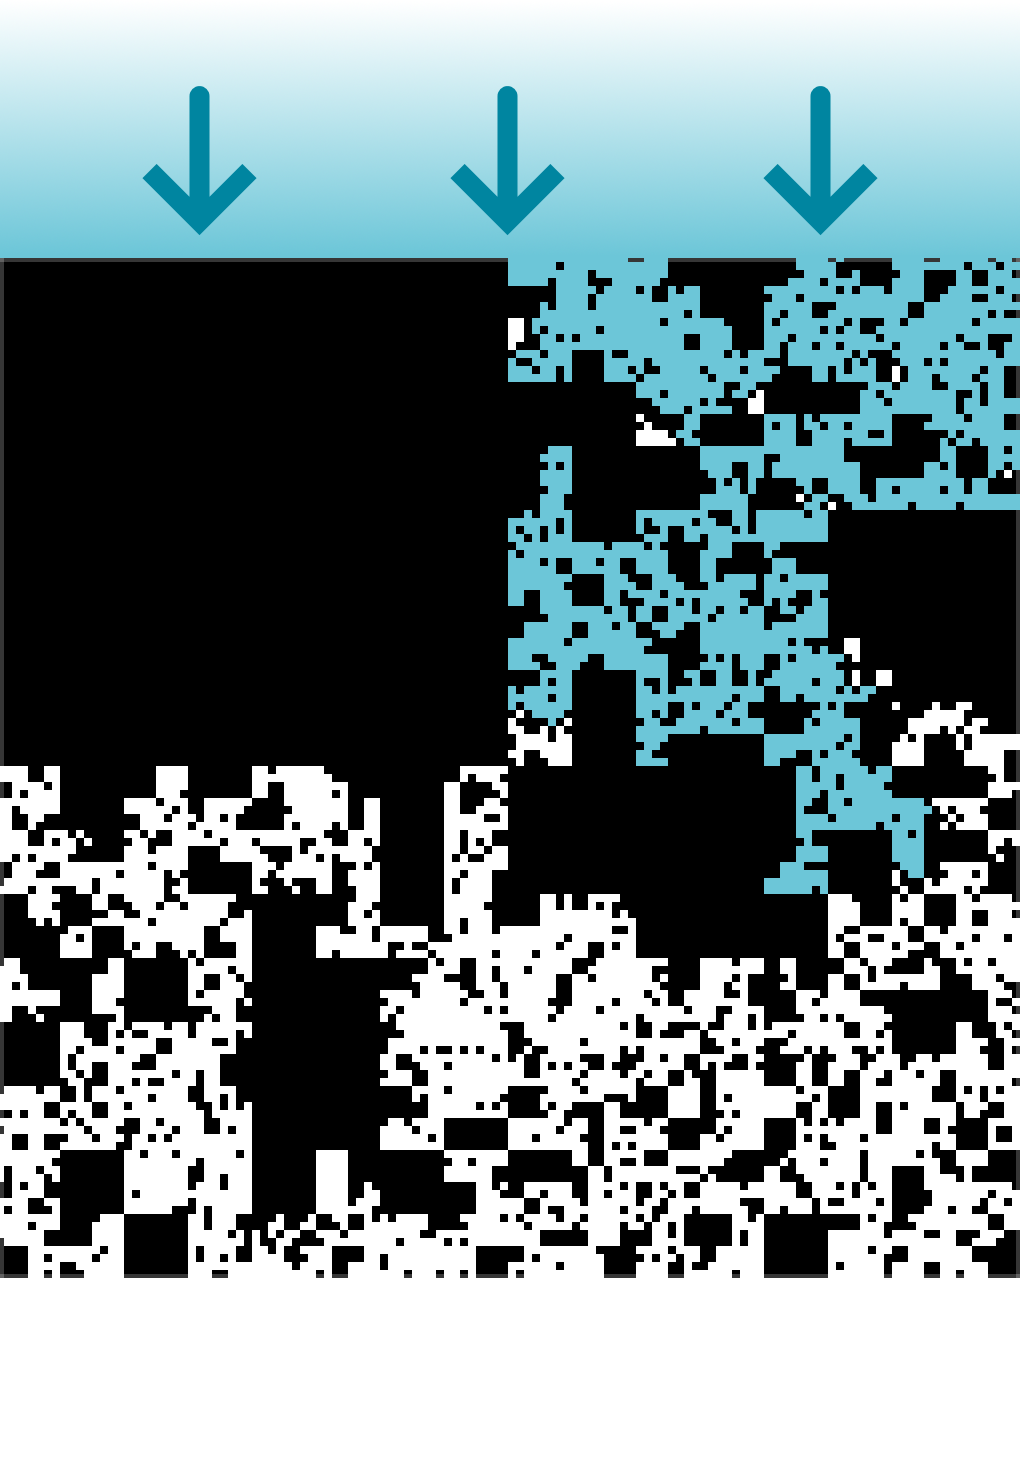
\includegraphics[width=4.2cm]{percolation_fluid}
		\centering
		\captionsetup{justification=centering}
		\caption{No vertical crossing: \\Fluid is stuck}
		\label{fig:percolationFluidNoCrossing}
	\end{subfigure}
	%\hspace{0.5cm}
	\begin{subfigure}{4.2cm}
		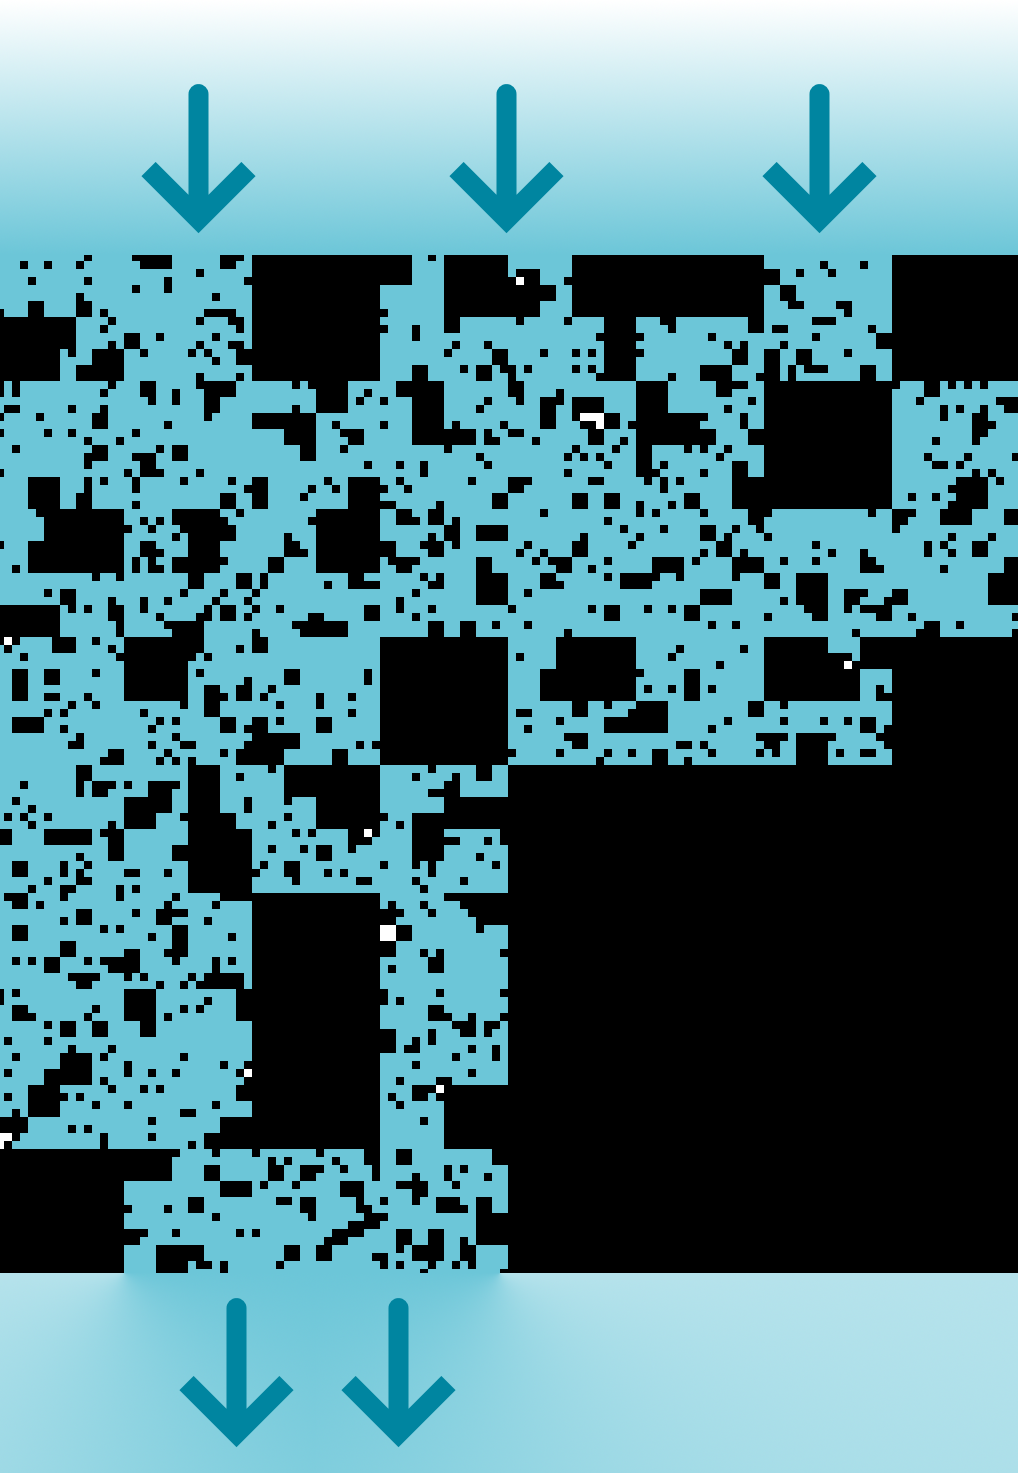
\includegraphics[width=4.2cm]{percolation_fluid_bis}
		\centering
		\captionsetup{justification=centering}
		\caption{Vertical crossings: \\Fluid can traverse}
		\label{fig:percolationFluidCrossing}
	\end{subfigure}
	\centering
	\caption{Percolations and Fluids}
	\label{fig:percolationFluid}
\end{wrapfigure}
\section{Percolation Crossings}
We are now interested in crossings from one side of the unit cuboid to the other side.
There is some physical motivation for such questions:
Suppose the percolation was a mathematical model for a physical material.
If $P$ has a crossing, then a fluid can pass through the material layer.
However, it will be stuck if there is no crossing.
The length of the crossing will tell how long it takes for the fluid to traverse the material.

The convention in mathematics is to study horizontal crossings, despite the more clear physical interpretation of vertical ones.
Rotating 90$^{\circ}$ transforms vertical crossings to horizontal ones and vice-versa, so studying either is equivalent.
We choose to stick to the mathematical convention.

\subsection{Types of Crossings}
There will be three types of crossing considered, according how the path of is allowed to behave.

Consider a percolation $P$ on the unit cuboid $\left[ 0,1 \right]^D$ in $D$ dimensions, and let $\gamma: \left[ 0,1 \right] \to \left[ 0,1 \right]^D$ be a crossing of the cuboid, i.e. $\gamma(0) \in \{ 0 \} \times \left[ 0,1 \right]^{D-1}$ and $\gamma(1) \in \{ 1 \} \times \left[ 0,1 \right]^{D-1}$.
In the case of a finite percolation\footnote{i.e. $P \sim \text{Perc}^D(n,p,d)$ with $n,d < \infty$}, we can view a crossing as a walk on the cuboids of side $\nicefrac{1}{n^d}$.

\paragraph{Straight}
The crossing is said to be straight if $\gamma(y) = y \times (x_2,\dots,x_D)$.
That is, if the path goes on a direct line from one side to the other.
Only one step direction is allowed.
%Refer to fig. \ref{fig:crossing-straight}.

\paragraph{Semi-Straight}
The crossing is said to be semi-straight if $\forall \, 0 \leq y < z \leq 1, \ \gamma(y)_0 < \gamma(z)_0$\footnote{Writing $\gamma(y)_0$ for the first component of $\gamma(y)$.}.
That is, if the path never goes backwards.
This allows steps in $2D-1$ direction: all the possible directions except $(-1,0,\dots,0)$.
%Refer to fig. \ref{fig:crossing-semi-straight}.

\paragraph{Non-Straight}
If the crossing is neither straight or semi-straight, then it is non-straight.
In the latter case, all steps directions are allowed.
%Refer to fig. \ref{fig:crossing-non-straight}.

The following (fig. \ref{fig:crossingTypes}) illustrate the different types of crossings in two dimensions (the easiest to picture), extension to greater dimensions is straightforward.
\begin{figure}[!h]
	\begin{subfigure}{0.3\linewidth}
		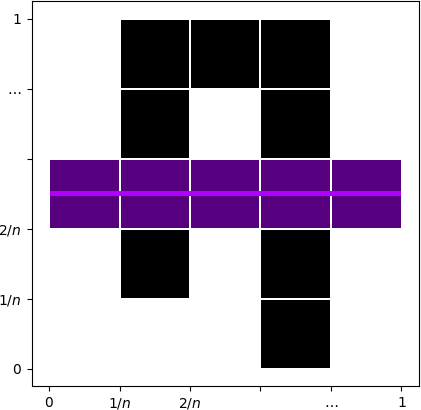
\includegraphics[width=5.4cm]{crossing-straight}
		\centering
		\captionsetup{justification=centering}
		\caption{Straight}
		\label{fig:crossingStraight}
	\end{subfigure}
	\hspace{0.04\linewidth}
	\begin{subfigure}{0.3\linewidth}
		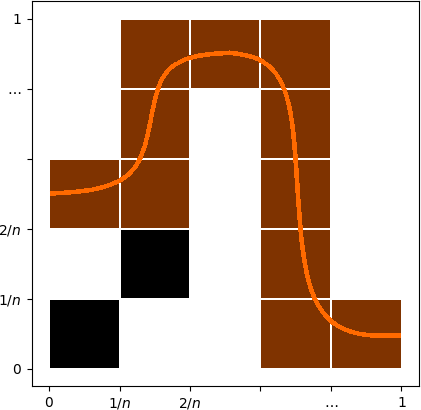
\includegraphics[width=5.4cm]{crossing-semi-straight}
		\centering
		\captionsetup{justification=centering}
		\caption{Semi-Straight}
		\label{fig:crossingSemiStraight}
	\end{subfigure}
	\hspace{0.04\linewidth}
	\begin{subfigure}{0.3\linewidth}
		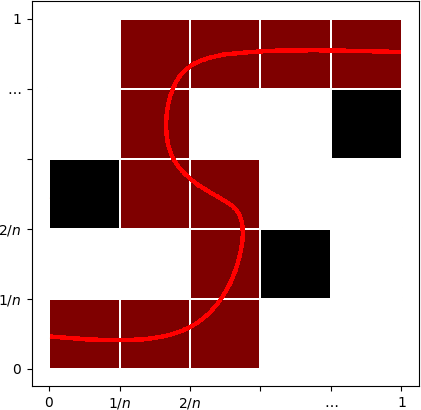
\includegraphics[width=5.4cm]{crossing-non-straight}
		\centering
		\captionsetup{justification=centering}
		\caption{Non-Straight}
		\label{fig:crossingNonStraight}
	\end{subfigure}
	\caption{Crossing types studied.}
	\label{fig:crossingTypes}
\end{figure}
When talking about a "crossing" in general, we will assume it may be either straight, semi-straight, or non-straight.


\subsection{Percolation Crossings}
First, we are interested in crossing lying on the percolation $P$.

\subsubsection{Crossings Probability}
For a percolation $P \sim \text{Perc}^D(n,p,d)$, we look at the probability that a crossing exist.

\paragraph{Straight Crossings}
This case is simple enough to derive an explicit formula for both classical and recursive percolations.
\subparagraph{Classical Percolation}
Take $P \sim \text{Perc}^D(\infty,p,1)$.
Then the probability that there is a straight crossing on the first line is $p^n$ (and is the same for the $n^{D-1}$ lines).
Thus, the probability that there is no crossing on any line is $1-(1-p^n)^{n^{D-1}}$, i.e. 
$$\mathbb{P}(P \text{ has a straight crossing}) = 1-(1-p^n)^{n^{D-1}} = \mathcal{O}(p^n f(n)) \text{ with } f(n) \text{ a polynomial of } n.$$
Thus, $\mathbb{P}(P \text{ has a straight crossing}) \to 0$, so it is almost sure that there is no crossing on a classical percolation $P$.

\subparagraph{Recursive Percolation}
Now take $P \sim \text{Perc}^D(n,p,\infty)$.

Let $Y^k$ be the number of straight crossings after $k$ filtrations, and $E^k = \mathbb{E}(Y^k)$ be the expected number of straight crossings\footnote{We count two crossings as different if they go through different cuboids.}.
Clearly, $E^0 = 1$, $E^1 = p^nn$, and recursively, $E^k = p^{n^k}nE^{k-1}$.
So in general, we get $E^k = n^k \prod_{i=1}^{k} p^{n^i}$, and $E^k \to 0$ as $k \to \infty$.
Now, $\mathbb{E}(Y^k) \to 0$ together with $Y^k \geq 0$ gives $\mathbb{P}(Y^k = 0) \to 1$.
So eventually, it is almost sure that a recursive percolation will have no straight crossings.

%\subparagraph{numrics}
%plots and plots comments
%explicit formula for straight crossings

\subsubsection{Crossings Length}
The length of a straight crossing is always 1.
However, for non-straight and semi-straight crossing, it is less clear.
We study this numerically.
%plots and plots comments

%\subsubsection{Crossings Dimension}
%plots and plots comments

\subsection{Percolation Complement Crossings}
We turn our interest to crossings on the complement $P^C = \left[ 0,1 \right]^D \setminus P$ for a recursive percolation $P \sim \text{Perc}^D(n,p,\infty)$.

\subsubsection{Crossings Probability}
Again, we will first be interested in the probability that a crossing exists.

\paragraph{Straight Crossings}
There is a straight crossing on the complement $P^C$ of the percolation if there exists a point $x \in \left[ 0,1 \right]^{D-1}$ such that $\left[ 0,1 \right] \times \{ x \}$  is in $P^C$, i.e. do not intersect with $P$.

The following result is inspired from \cite[p.309 b.(1)]{Chayes_1988} and \cite[p.215]{Mandelbrot_1982}.
Suppose $x = (x_2,\dots,x_D)$ with $x_i \neq \nicefrac{j_i}{n^k} \text{ for } j_i \in \llbracket 0,n^k \rrbracket$\footnote{Writing $\llbracket a,b \rrbracket$ for $\Z \cap \left[ 0,n^d \right]$.}.
Then if $p \leq \nicefrac{1}{n}$ we have that almost surely, $P$ has a complement crossing along $\left[ 0,1 \right] \times \{ x \}$.
This is in fact equivalent to 
$$\mathbb{P}\left( \left( P \cap \left[ 0,1 \right] \times \{ x \} \right) = \emptyset \right) = 1 .$$
\begin{proof}
	Let $x \neq \left( \frac{j_2}{n^k},\dots,\frac{j_D}{n^k} \right) \text{ for any } j_i \in \llbracket 0,n^k \rrbracket$.
	The number of intervals of the form $\left[ \frac{j_1-1}{n^k},\frac{j_1}{n^k} \right] \times \{ x \}$ still in the percolation at depth $k$ is a branching process in which each interval has $np$ offspring.
	Thus, the branching process dies out almost surely if $np \leq 1$, i.e. $p \leq \nicefrac{1}{n}$.
	When the process dies, we have $\left[ 0,1 \right] \times \{ x \} \subseteq P^C$, so there is a crossing in the complement of $P$.
\end{proof}

%plots
%comments

\paragraph{Non-Straight Complement Crossings}
There will be a non-straight crossing in the percolation complement almost surely if $p \leq \frac{1}{\sqrt[2(D-1)]{n}}$\footnote{Where $\sqrt[2(D-1)]{n}$ is the $2(D-1)^{th}$ root of $n$.}.
The following proof extends techniques from \cite[p.310 b.(2)]{Chayes_1988}.
\begin{proof}\label{prf:nonStraightComplementCrossigs}
	This time, take $x = \left( \frac{j_2}{n^k},\dots,\frac{j_D}{n^k} \right) \text{ with } j_i \in \llbracket 1,n^k-1 \rrbracket$, $x_i = \nicefrac{j_i}{n^k}$.
	Call a segment $\left[ \frac{j_1-1}{n^k},\frac{j_1}{n^k} \right] \times \{ x \}$ vacant if any of the $2(D-1)$ cuboids adjacent at the depth $k$ of the percolation have been removed.
	
	Let $Y^k$, be the number of occupied segments of the form $\{ x \} \times \left[ \frac{j_1-1}{n^k},\frac{j_1}{n^k} \right]$ at depth $k$.
	Then $Y^k$, is a branching process in which each the mean number of offspring is $p^{2(D-1)n}$.
	This branching process is almost surely eventually empty if $np^{2(D-1)} \leq 1$, i.e. if $p \leq \frac{1}{\sqrt[2(D-1)]{n}}$.
	
	Suppose the branching process dies at depth $k$.
	Then there are only finitely many points of the form $\left( \nicefrac{j_1}{n^k}, x_2,\dots,x_D \right) \text{ s.t. } j_1 \in \llbracket 1,n^k-1 \rrbracket$.
	It is almost sure that eventually, all the cuboids touching these points will be removed (since they are kept with a probability $p<1$ after each filtration).
	Once this is the case, there is a crossing path from $\left( 0, x_2,\dots,x_D \right)$ to $\left( 1, x_2,\dots,x_D \right)$ that zigzags near the segment $\left[ 0,1 \right] \times \{ x \}$ (see fig. \ref{fig:complementCrossing} for illustrations in two and three dimensions).
\end{proof}

\begin{figure}[!h]
	\vspace{-0.75cm}
	\begin{subfigure}{0.44\linewidth}
		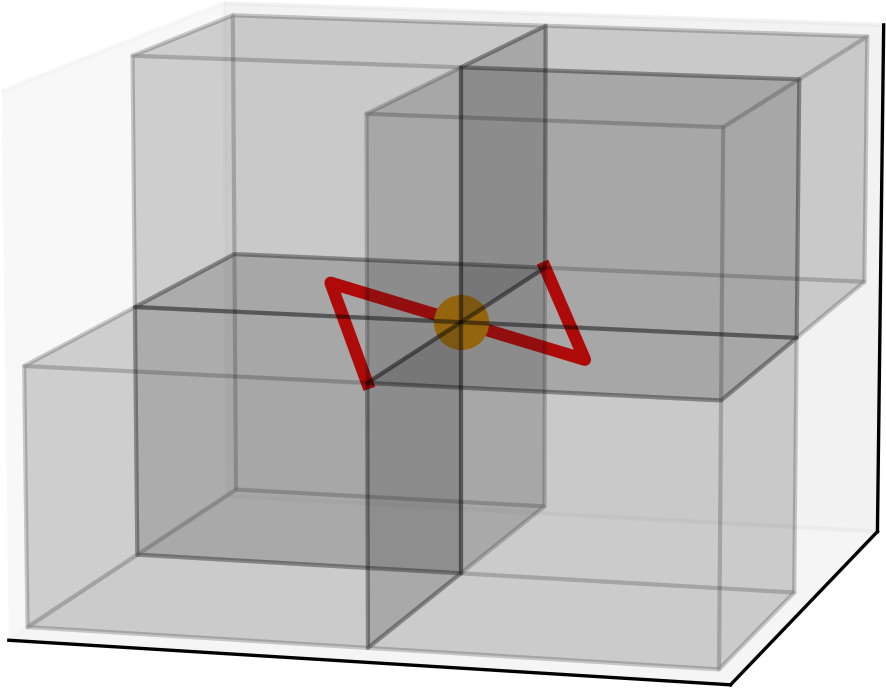
\includegraphics[width=5.25cm]{complement_crossing3D}
		\centering
		\captionsetup{justification=centering}
		\caption{$D = 3$}
		\label{fig:complementCrossing3D}
	\end{subfigure}
	\hspace{0.1\linewidth}
	\begin{subfigure}{0.44\linewidth}
		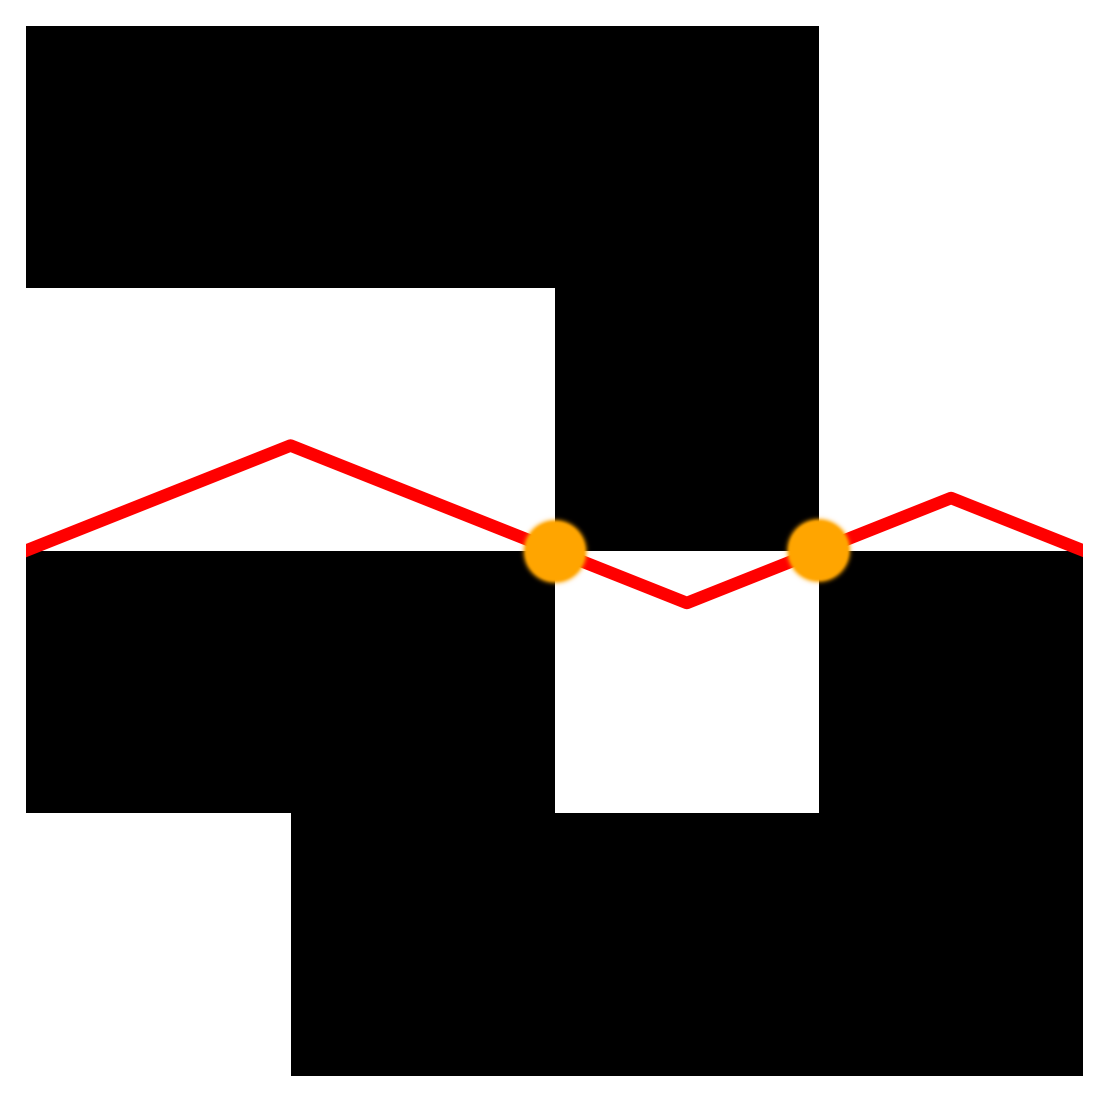
\includegraphics[width=5.25cm]{complement_crossing2D}
		\centering
		\captionsetup{justification=centering}
		\caption{$D = 2$}
		\label{fig:complementCrossing2D}
	\end{subfigure}
	\centering
	\caption{Eventually, the cuboids touching the orange point(s) will be removed and the red path will remain in full within the percolation complement.}
	\label{fig:complementCrossing}
\end{figure}

\subsubsection{Crossings Length}
%plots and plots comments

%\subsubsection{Crossings Dimension}
%plots and plots comments

\subsection{Link Between Crossings and Complement Crossings}
In the case of $D=2$, vertical (respectively horizontal) crossing on $P$ is incompatible with horizontal (respectively vertical) crossing of $P^C$.

Since we proved that if $p \leq \nicefrac{1}{\sqrt{n}}$, then $P^C$ has a crossing with probability one, we get as a consequence that $P$ have a crossing with probability zero (note that the existence probability of a vertical crossing is the same as the one of an horizontal crossing, by symmetry).

\subsection{Connectivity Properties}
Some properties of percolations are already known by the community.
We will look at here the ones regarding connectivity of the percolation, which are related to crossings.
Most results were stated in two dimensions in the literature.
When possible, we will generalize the results to dimension $D$.

\paragraph{Almost Sure Disconnectedness}
If $p \leq \nicefrac{1}{\sqrt{n^{D-1}}}$, then the largest connected component in a percolation $P \sim \text{Perc}^D(n,p,\infty)$ is a point (almost surely).

The following proof uses techniques from \cite[p.310 b.(2)]{Chayes_1988}
\begin{proof}
	Similarly to last proof (see section \ref{prf:nonStraightComplementCrossigs}), we say that a facet 
	$$f_{j_1,\dots,j_D}^k = \left\lbrace \frac{j_1}{n^k} \right\rbrace \times \left( \prod_{i=2}^{D} \left[ \frac{j_i-1}{n^k},\frac{j_i}{n^k} \right] \right) $$
	is vacant is either of the two adjacent cuboids in the $k^{th}$ filtration is.
	
	Let $Y^k$ be the number of occupied facets for the form $f_{j_1,\dots,j_D}^k$ after $k$ filtrations.
	$Y^k$ is a branching process in which each element has $p^2n^{D-1}$ offspring.
	Now, if $p^2n^{D-1}	\leq 1$ (i.e. $p \leq \nicefrac{1}{\sqrt{n^{D-1}}}$), then the branching process will die out with probability one.
	Similarly to last proof, if we wait long enough, it is almost sure that there will be a hyper-surface\footnote{Here, hyper-surface and hyperplane are of dimensions $D-1$ in $\R^D$.} in the percolation complement $P^C$ arbitrarily close to the hyperplane $\left\lbrace \frac{j_1}{n^k} \right\rbrace \times \left[ 0,1 \right]^{D-1}$ (see fig. \ref{fig:complementSurface} for examples in two and three dimensions).
	
	Finally, repeating the argument for $j_m \in \left[ 1,n^k\right] $, we get that almost surely, there are hyper-surfaces on the percolation complement arbitrarily close to the hyperplanes $\left\lbrace \frac{j_1}{n^k} \right\rbrace \times \left[ 0,1 \right]^{D-1}$.
	By reflecting the argument, there are some hyper-surfaces arbitrarily close to the hyperplanes $\left[ 0,1 \right]^{m-1} \times \left\lbrace \frac{j_m}{n^k} \right\rbrace \times \left[ 0,1 \right]^{D-m-1}$.
	Therefore, the largest connected component is a point.
\end{proof}

\begin{figure}[!h]
	\vspace{-0.75cm}
	\begin{subfigure}{0.44\linewidth}
		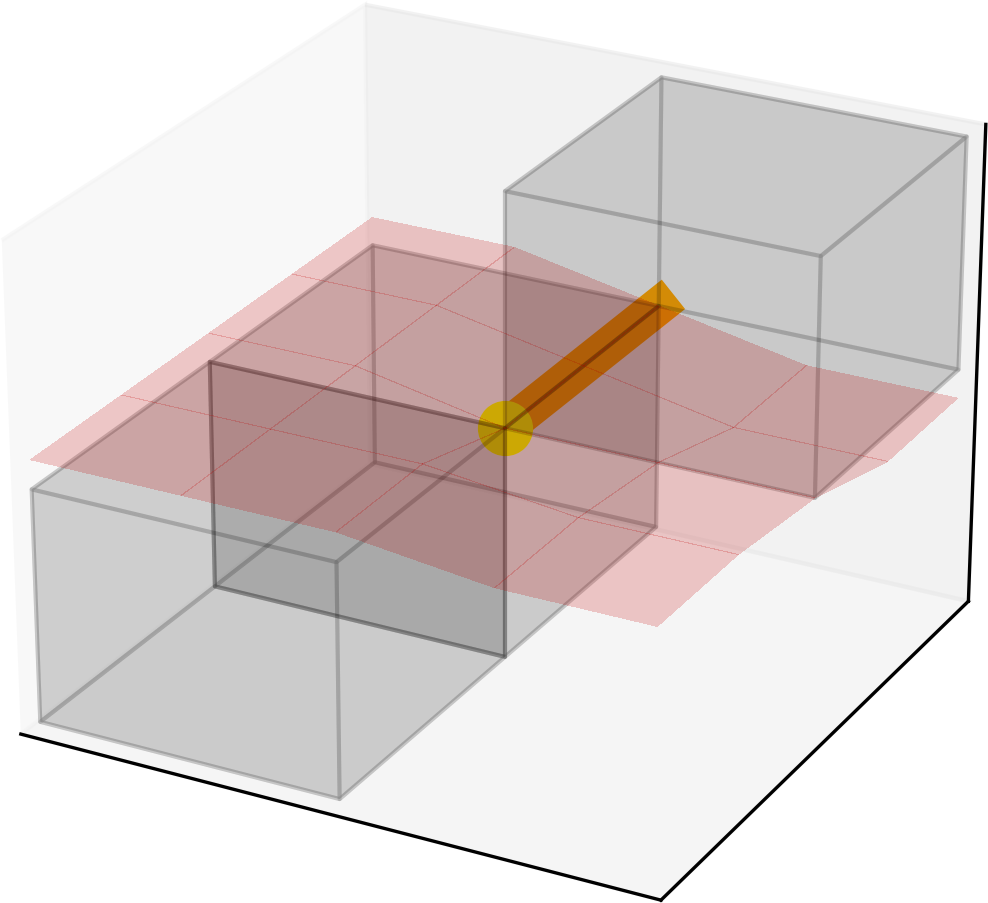
\includegraphics[width=5.25cm]{complement_surface3D}
		\centering
		\captionsetup{justification=centering}
		\caption{$D = 3$\\Hyper-surface is a usual 3D surface.}
		\label{fig:complementSurface3D}
	\end{subfigure}
	\hspace{0.1\linewidth}
	\begin{subfigure}{0.44\linewidth}
		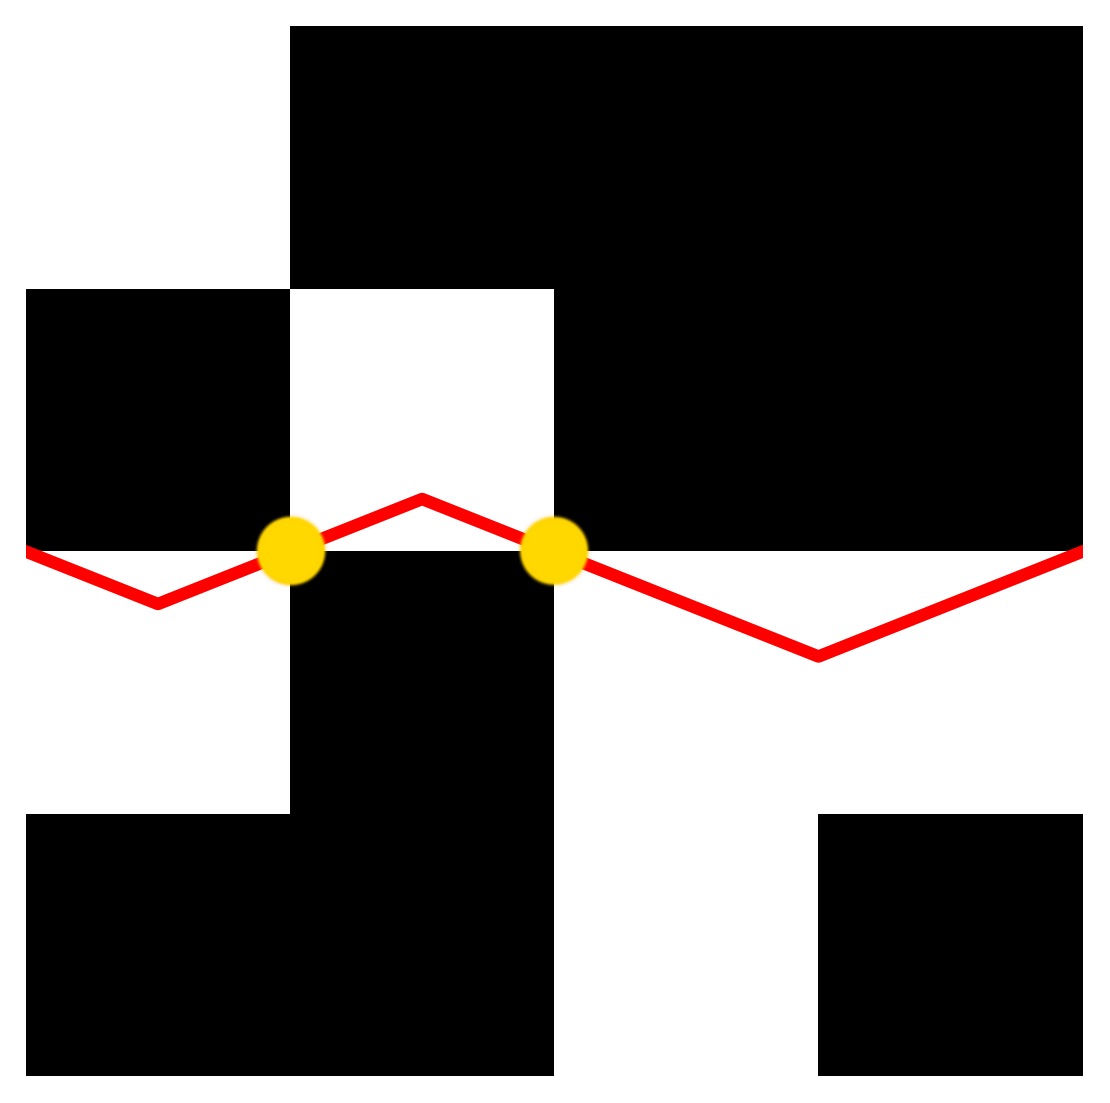
\includegraphics[width=5.25cm]{complement_surface2D}
		\centering
		\captionsetup{justification=centering}
		\caption{$D = 2$\\Hyper-surface is just a line.}
		\label{fig:complementSurface2D}
	\end{subfigure}
	\centering
	\caption{Eventually, the cuboids touching the orange line and yellow point(s) will be removed and the red hyper-surface will remain in full within the percolation complement.}
	\label{fig:complementSurface}
\end{figure}

\paragraph{Minimal Parameter for Crossings to Appear}
It is interesting to study when the percolation starts having crossings.
One defines (notation introduced in \cite{Chayes_1988}) $p_c$ as the minimum value of $p$ such that $P \sim \text{Perc}^D(n,p,\infty)$ has a non zero probability to have a crossing, i.e.
$$p_c = \inf \left\lbrace p \mid \mathbb{P}(P \text{ has a crossing})>0 \right\rbrace .$$

It is reasonable to conjecture that $p_c<1$ for all $n,D \geq 2$. In fact, this was proved in the case $D=2$ in \cite{Chayes_1988}.

Narrowing down to $D=2$:
Chayes et al. proved in \cite{Chayes_1988} that almost surely, if $p<p_c$, the largest connected component of $P$ is a point.
For $p \geq p_c$, the largest connected component is almost surely not a point.
Moreover, we pave $\R^2$ with a percolation $P \sim \text{Perc}^D(n,p,\infty)$ attached at each point of $\Z^2$ (and calling this $P'$).
Then, with probability one, $P'$ has a unique unbounded connected component.
This explains the "jump" behaviour observed in section \ref{blob}.

	%% !TeX spellcheck = en_GB
\section{Projections}

%intersection as intro?
\subsection{2D to 1D}
%plots and plots comments
\subsection{3D to 2D}
%plots and plots comments
\subsection{3D to 1D}
%plots and plots comments
\subsection{Dimension of the (non void) Universe}
%Link with physics





	% !TeX spellcheck = en_GB
\section{Conclusion}
%\subsection{Summary}
We have studied percolation fractals in the most general form (starting from a $D$ dimensional cuboid).
Classical percolation almost surely have the same dimension as the initial set\footnotemark, while recursive percolation have almost sure dimension in $\left[ 0, D \right)$
\addtocounter{footnote}{-1}
\footnotemark
\footnotetext{For $p \in \left( 0,1 \right)$.}.
We have proved that recursive percolations reach a density of zero eventually, almost surely, and is totally disconnected when $p$ is small enough\footnote{When $p \leq \nicefrac{1}{\sqrt{n^{D-1}}}$.}.

We also studied the probability of the existence of a crossing. The latter having physical motivation\footnote{Being that if the percolation represents a porous material, the presence of a crossing tell if it is fluid-proof.})
The complexity of this problem pushed us to make numerical simulations.
We reduced our study to cases in two and three dimensions, and developed efficient algorithms to get the most reliable results (by increasing the number of experiments)\footnote{All results are aggregated at \url{https://pauldubois98.github.io/PercolationFractalsStudy/}.}.

%\subsection{Future Work}
In the future, it could be interesting to examine the dimensionality of the crossing path.
We anticipate the dimension will be one when the path is nearly straight, but this may increase for more irregular path.
The dimension of the path could be a good measure of the physical difficulty for a fluid to traverse the material.
This, together with the viscosity of the fluid could be interpreted as the strength of fluid flow traversing the medium.

It would also be interesting to see the effect of removing other shapes from the initial cuboid.
For example, many porous materials have round (or spherical) holes. It would therefore make sense to study percolations where the set removed is a $D$ dimensional ball, rather than a $D$ dimensional cuboid, as we have done so far.
This would make the model more complicated, but also more accurate in terms of physical interpretation.

	
	\bibliography{references}
	
	\appendix
	\clearpage\null\newpage
\begin{titlepage}
	\newcommand{\HRule}{\rule{\linewidth}{0.5mm}}
		\begin{center}
		
\includegraphics[scale=0.08]{oxford_logo.png}
		\vspace*{1cm}
		
		\textsc{\LARGE University of Oxford}\\[0.75cm]
		\textsc{\LARGE Mathematical Institute}
		
		\vspace{1.5cm}
		
		\HRule
		\vspace{0.75cm}
		
		\textit{\LARGE Random Fractals}
		\vspace{0.5cm}
		
		\textbf{\huge Appendix}
		
		\vspace{0.5cm}
		\HRule
		
		\vspace{1.5cm}
		
		\begin{minipage}{0.4\textwidth}
			\begin{flushleft}
				\large
				%\textit{Author}\\ Paul \textsc{Dubois}
			\end{flushleft}
		\end{minipage}
		
		\begin{minipage}{0.4\textwidth}
			\begin{flushright}
				\large
				%\textit{Supervisor}\\ Ben \textsc{Hambly}
			\end{flushright}
		\end{minipage}
		
		\vspace{0.5cm}
		
		\textit{Candidate Number}\\
		1051774
		
		\vspace{0.5cm}
		
		\textit{Course}\\
		MSc Mathematical Sciences
		
		\vfill
		
		{\large Trinity Term\\
			April 26, 2021}
	\end{center}
\end{titlepage}
	% !TeX spellcheck = en_GB
\section{More on Fractals}
Here will be discussed some extensions of famous fractals studied before (in section \ref{fractalsExamples}).
This is not directly relevant for this paper, but an involved reader may be interested.

\begin{wrapfigure}{r}{5.5cm}
	\vspace{-1.5cm}
	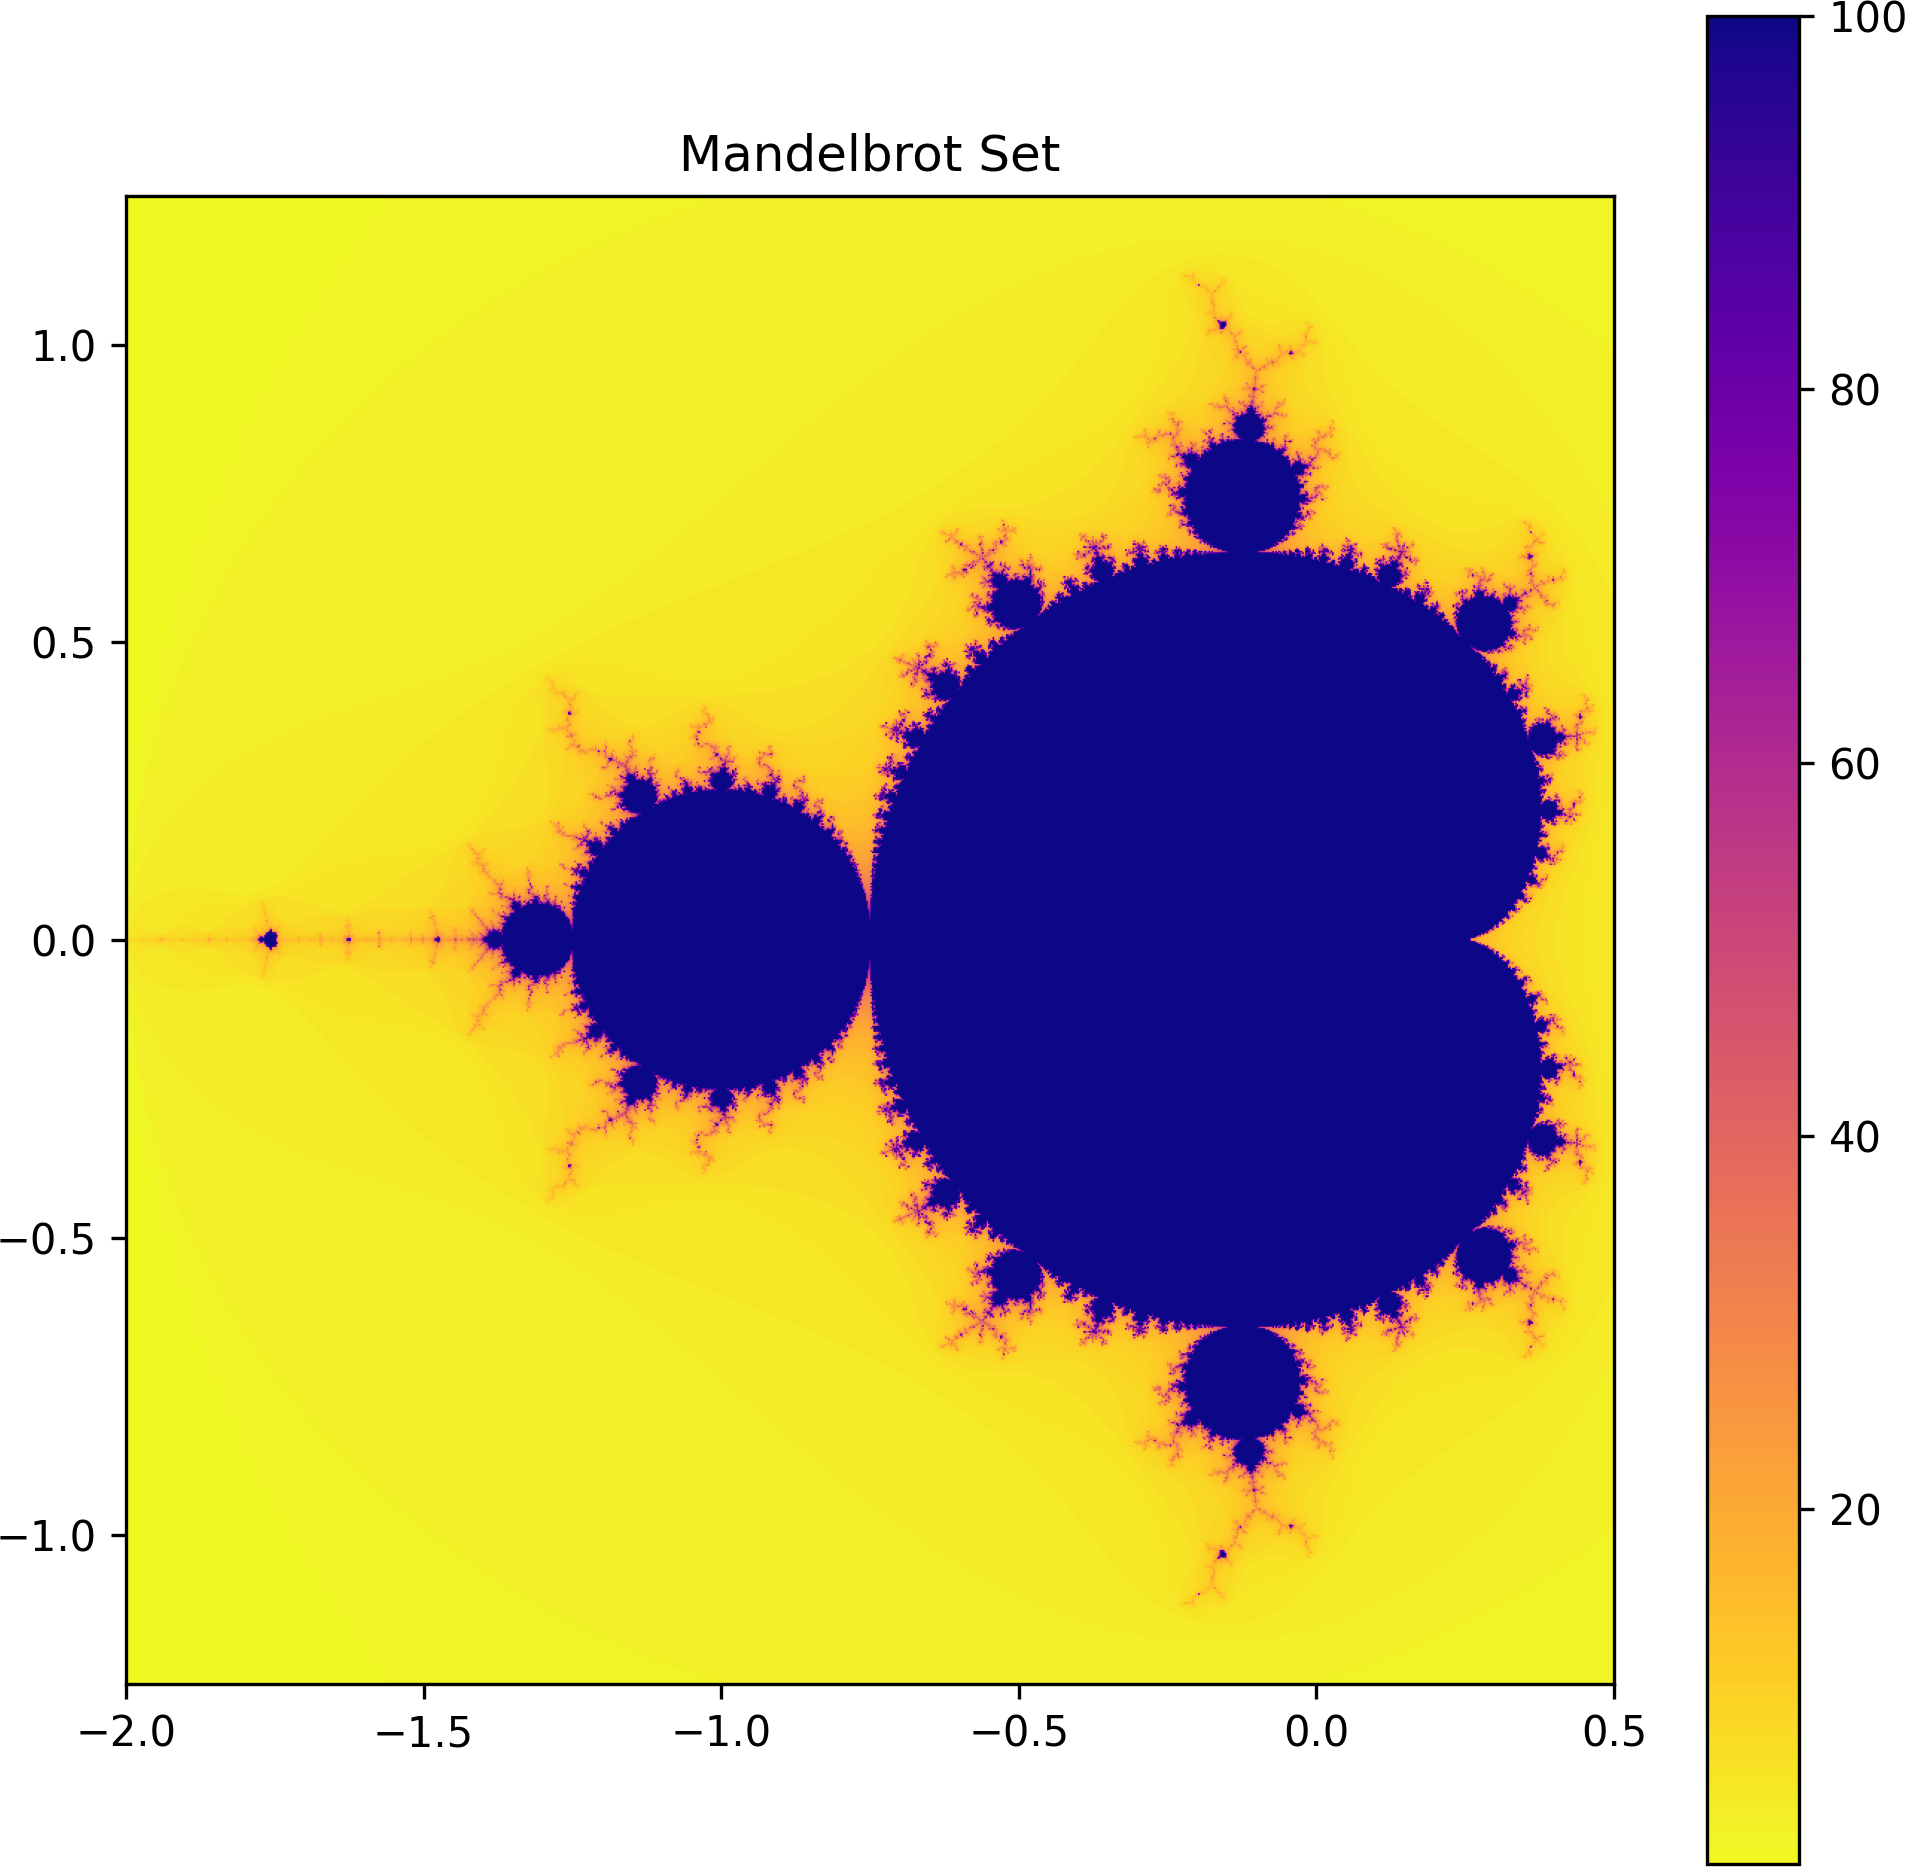
\includegraphics[width=5.5cm]{MandelbrotSet_colorbar}
	\centering
	\captionsetup{justification=centering}
	\caption{Mandelbrot Set}
	\label{fig:MandelbrotSetColorbar}
\end{wrapfigure}
\subsection{Mandelbrot and Julia Sets}
Mandelbrot and Julia sets involve calculating the limit of a sequence to determine if a point is in the set or not.
More precisely, one needs to determine whether the sequence diverges or not.
It is impossible to do such calculations with a computer, therefore, we approximate.
For each initial value $z_0$, we calculate the first values of the sequence.
We stipulate that the time taken by the sequence to reach $|z_n|>R$ is an indication of how fast the sequence diverges.

The plots are then made as follows:
we calculate the first $M$ values of the sequence.
If $|z_n|>R$ for some $n<M$, then let $g(z_0) = n$, with $n$ the smallest such integer.
If $|z_n| \leq R$ for all $n<M$, then let $g(z_0) = M$.
Finally, plot $g$ on the area $S \subseteq \C$ of interest.

On the figures \ref{fig:MandelbrotSet} and \ref{fig:JuliaSets}, the settings are $R=2$ and $M=100$.
The plots represent the value of $g$ through colours, with the same colour-bar as in fig. \ref{fig:MandelbrotSetColorbar}.


\subsection{Sierpiński Fractals}
Following the idea of the Sierpiński carpet, several fractals may be generated.
First, using (equilateral) triangles instead of squares:

\begin{wrapfigure}{r}{5cm}
	\vspace{-0.5cm}
	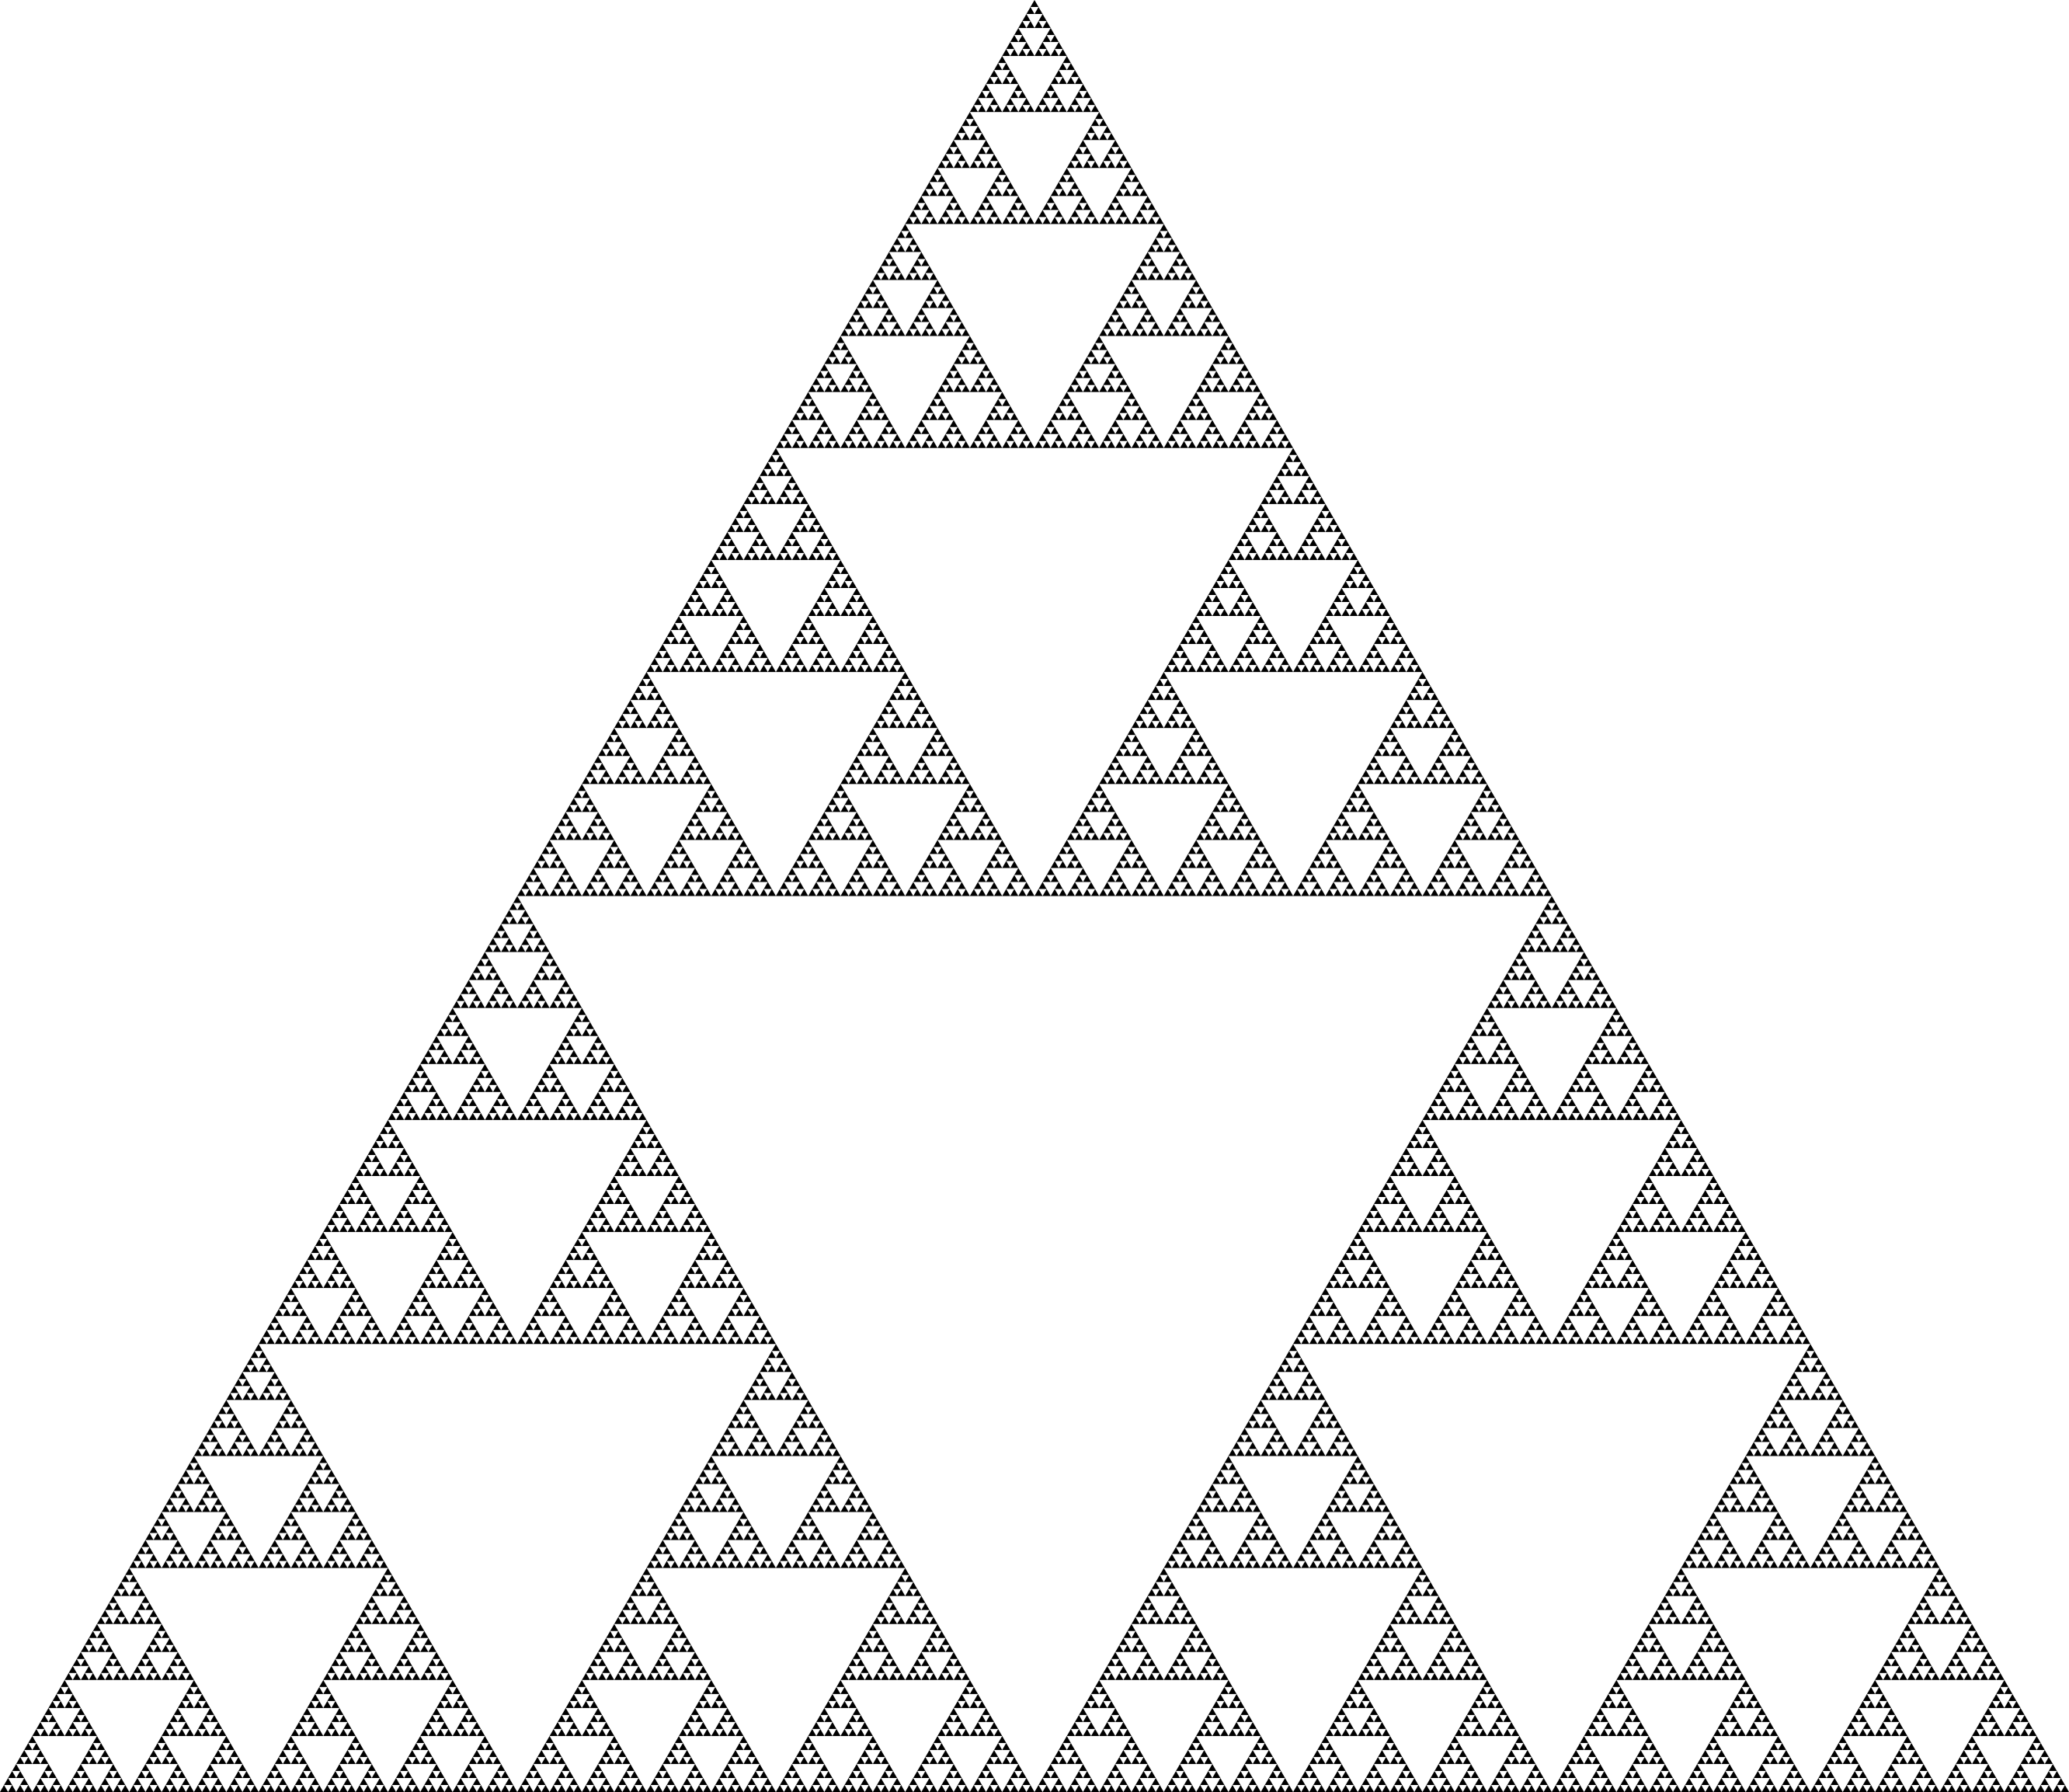
\includegraphics[width=6cm]{SierpinskiTriangle}
	\centering
	\captionsetup{justification=centering}
	\caption{Sierpinski Triangle (8 steps)}
	\label{fig:SierpinskiTriangle}
	\vspace{-3cm}
\end{wrapfigure}
\subparagraph{Sierpiński Triangle}
Sierpiński triangle is also a fractal constructed recursively by removing parts of its initial set, following a pattern similar to the one for Sierpiński carpet (although, there are equivalent definitions).

The construction starts from an equilateral triangle.
Then, at each step, split every equilateral triangle into 4 sub-triangles as follows:\\
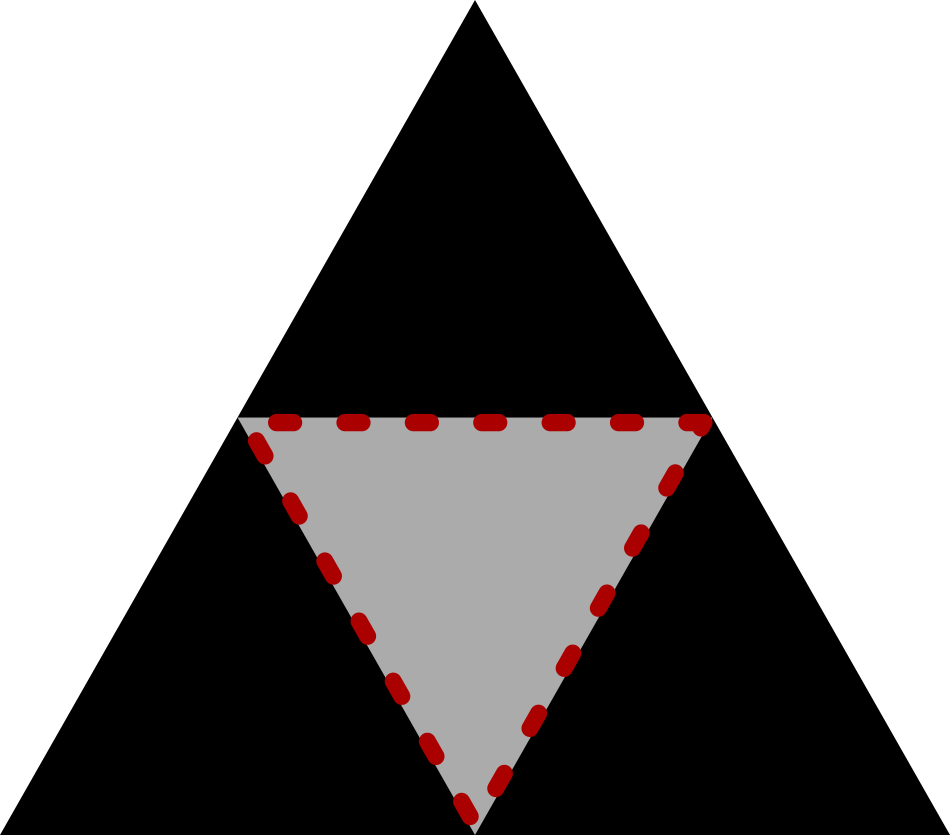
\includegraphics[width=4cm]{SierpinskiTriangleStep}\\
Remove the central triangle, and repeat the operation on the remaining 3 triangles.

The figure is made of $3$ copies of itself, scaled by a factor of $\frac{1}{2}$.
Therefore, the intuitive Hausdorff dimension for this set is $\dim_H(K) = \frac{log(3)}{log(2)} \approx 1.585$.
Again, this can be proved rigorously using similar techniques as in \cite[p. 34-35, ex. 2.7]{Falconer_1990}.

\paragraph{Sierpiński 3D Fractals}
As seen previously, the Sierpiński carpet and triangle live in a 2D world, but the idea of Sierpiński fractals may also be extended to 3D.

\subparagraph{Menger sponge}
The Menger sponge is the generalisation of Sierpiński carpet to 3 dimensions.

Start with a cube; split it into 27 identical copies scaled by $\frac{1}{3}$, and remove the central one, and the 6 cubes sharing a face with this central cube.
Repeat this operation on each of the 20 remaining cubes.

From this construction arise a fractal with dimension $\frac{log(20)}{log(3)} \approx 2.727$.

\subparagraph{Sierpiński tetrahedron}
The Sierpiński tetrahedron (or tetrix) is the analogue of Sierpiński triangle in 3 dimensions.
Start with a regular tetrahedron; split it into 5 identical copies scaled by $\frac{1}{2}$, and remove the central one.
Repeat this operation on each of the 4 remaining tetrahedrons.

From this construction arise a fractal with dimension $\frac{log(4)}{log(2)} = 2$.
Note that this set is dimension exactly 2 while not being a surface.

\begin{figure}[!h]
	\centering
	\begin{subfigure}{.24\textwidth}
		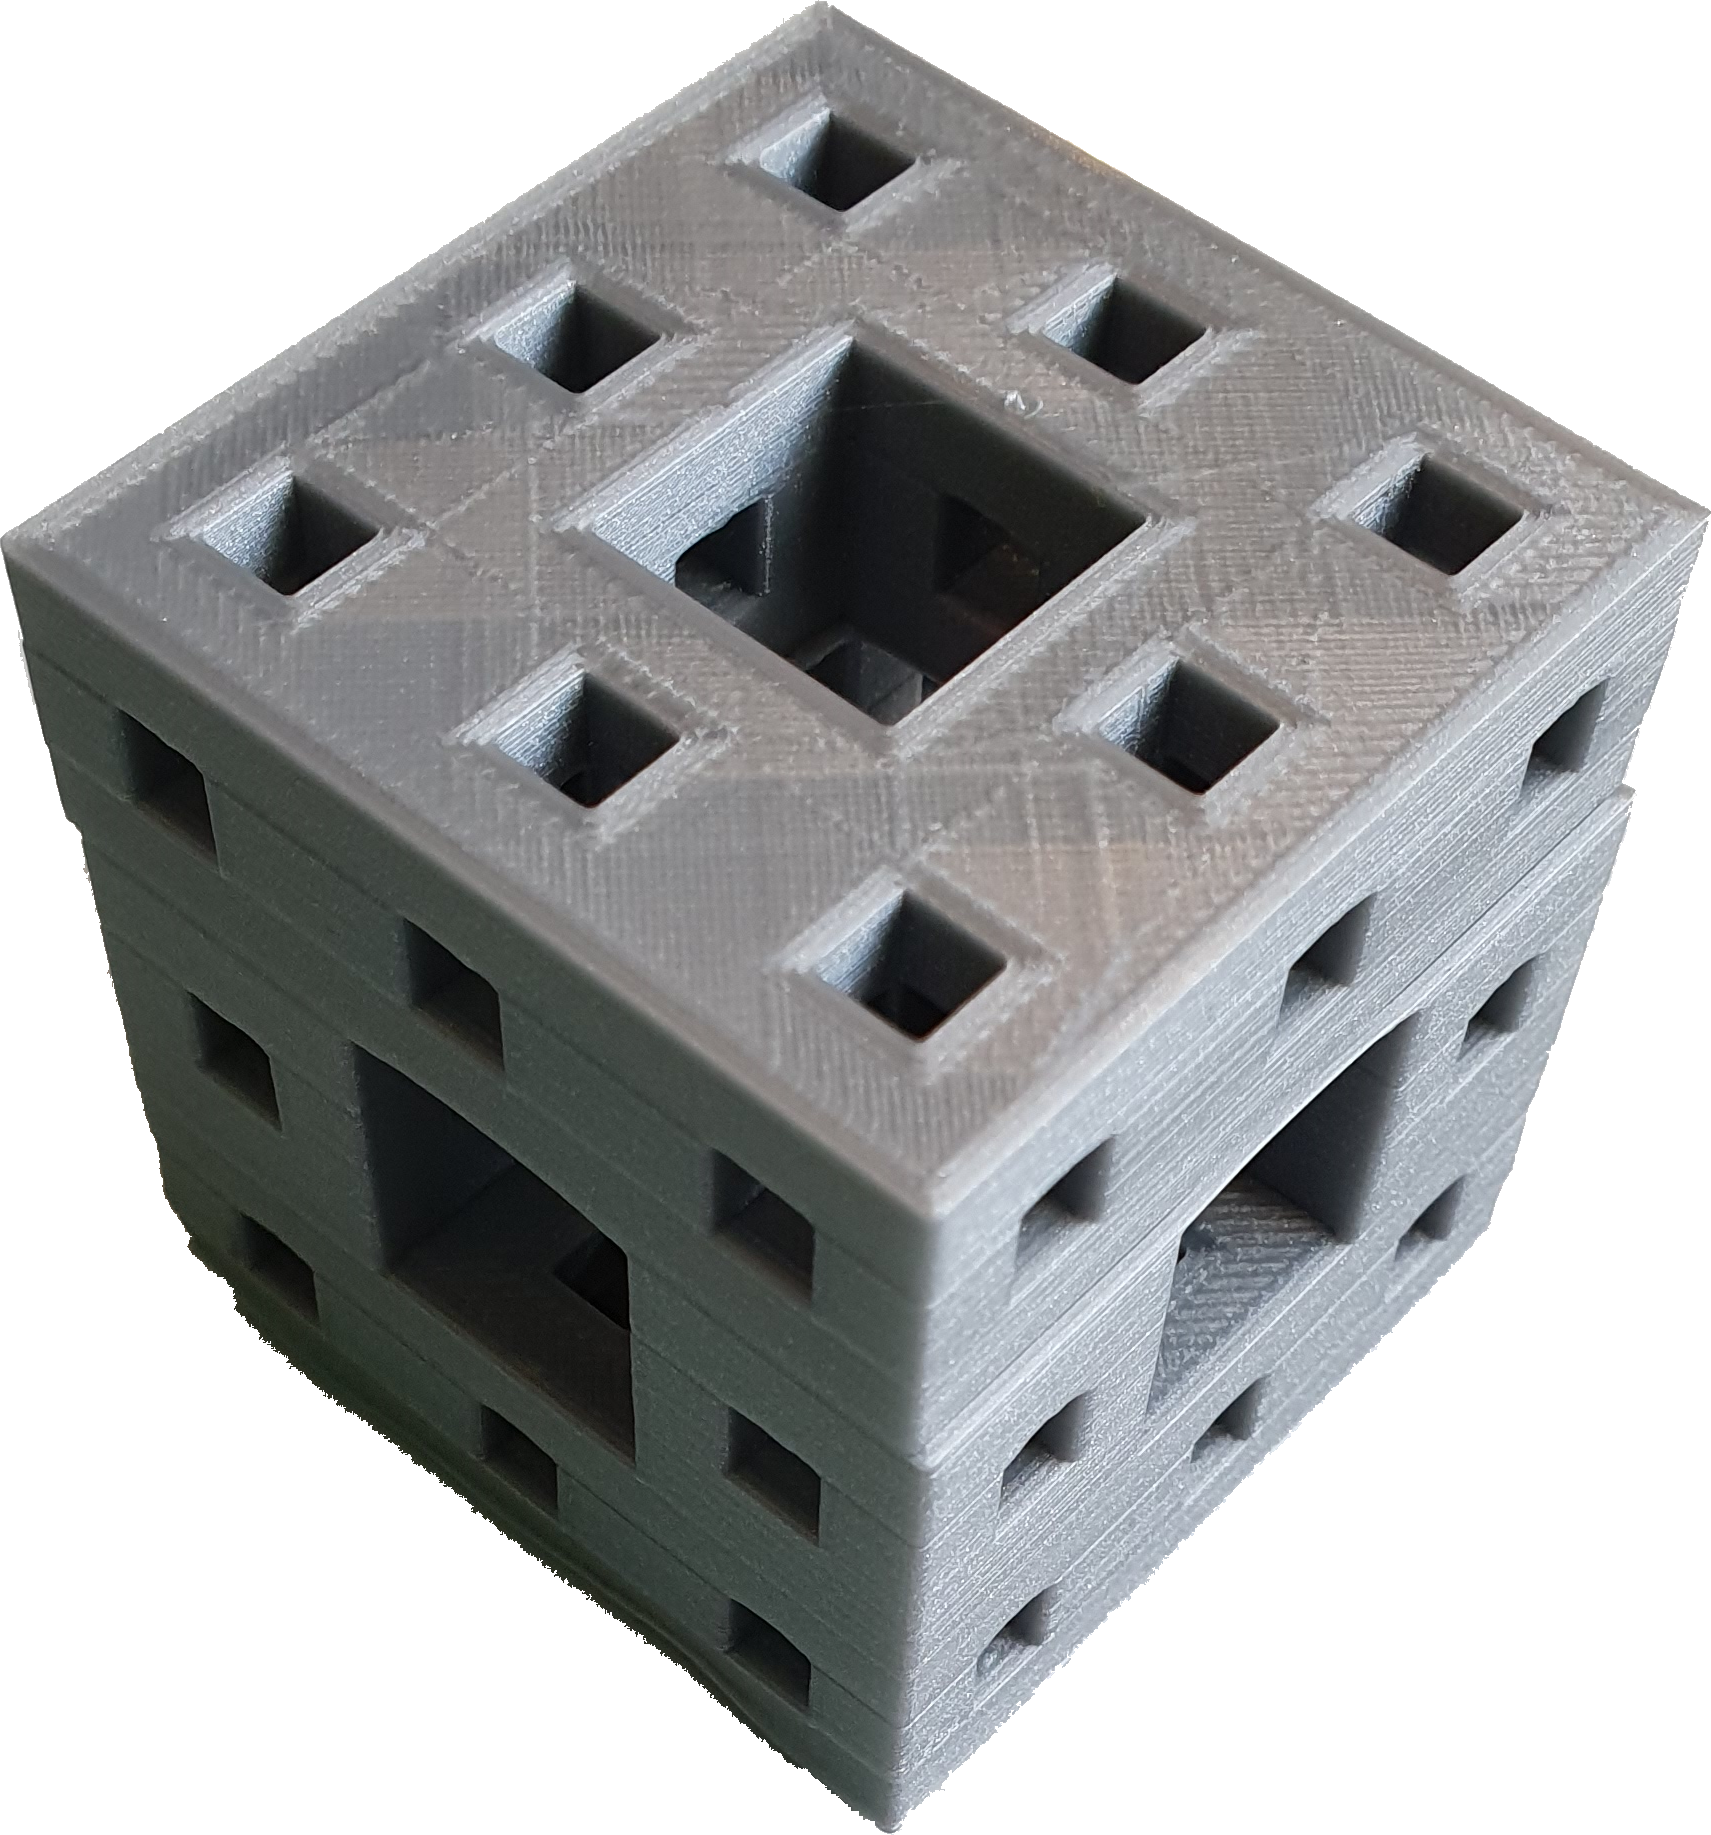
\includegraphics[width=3.25cm]{MengerSpongePhysics}
		\centering
		\captionsetup{justification=centering}
		\caption{Menger Sponge\\ 3D Printed (2 steps)}
		\label{fig:MengerSponge3Dprinted}
	\end{subfigure}
	\begin{subfigure}{.24\textwidth}
		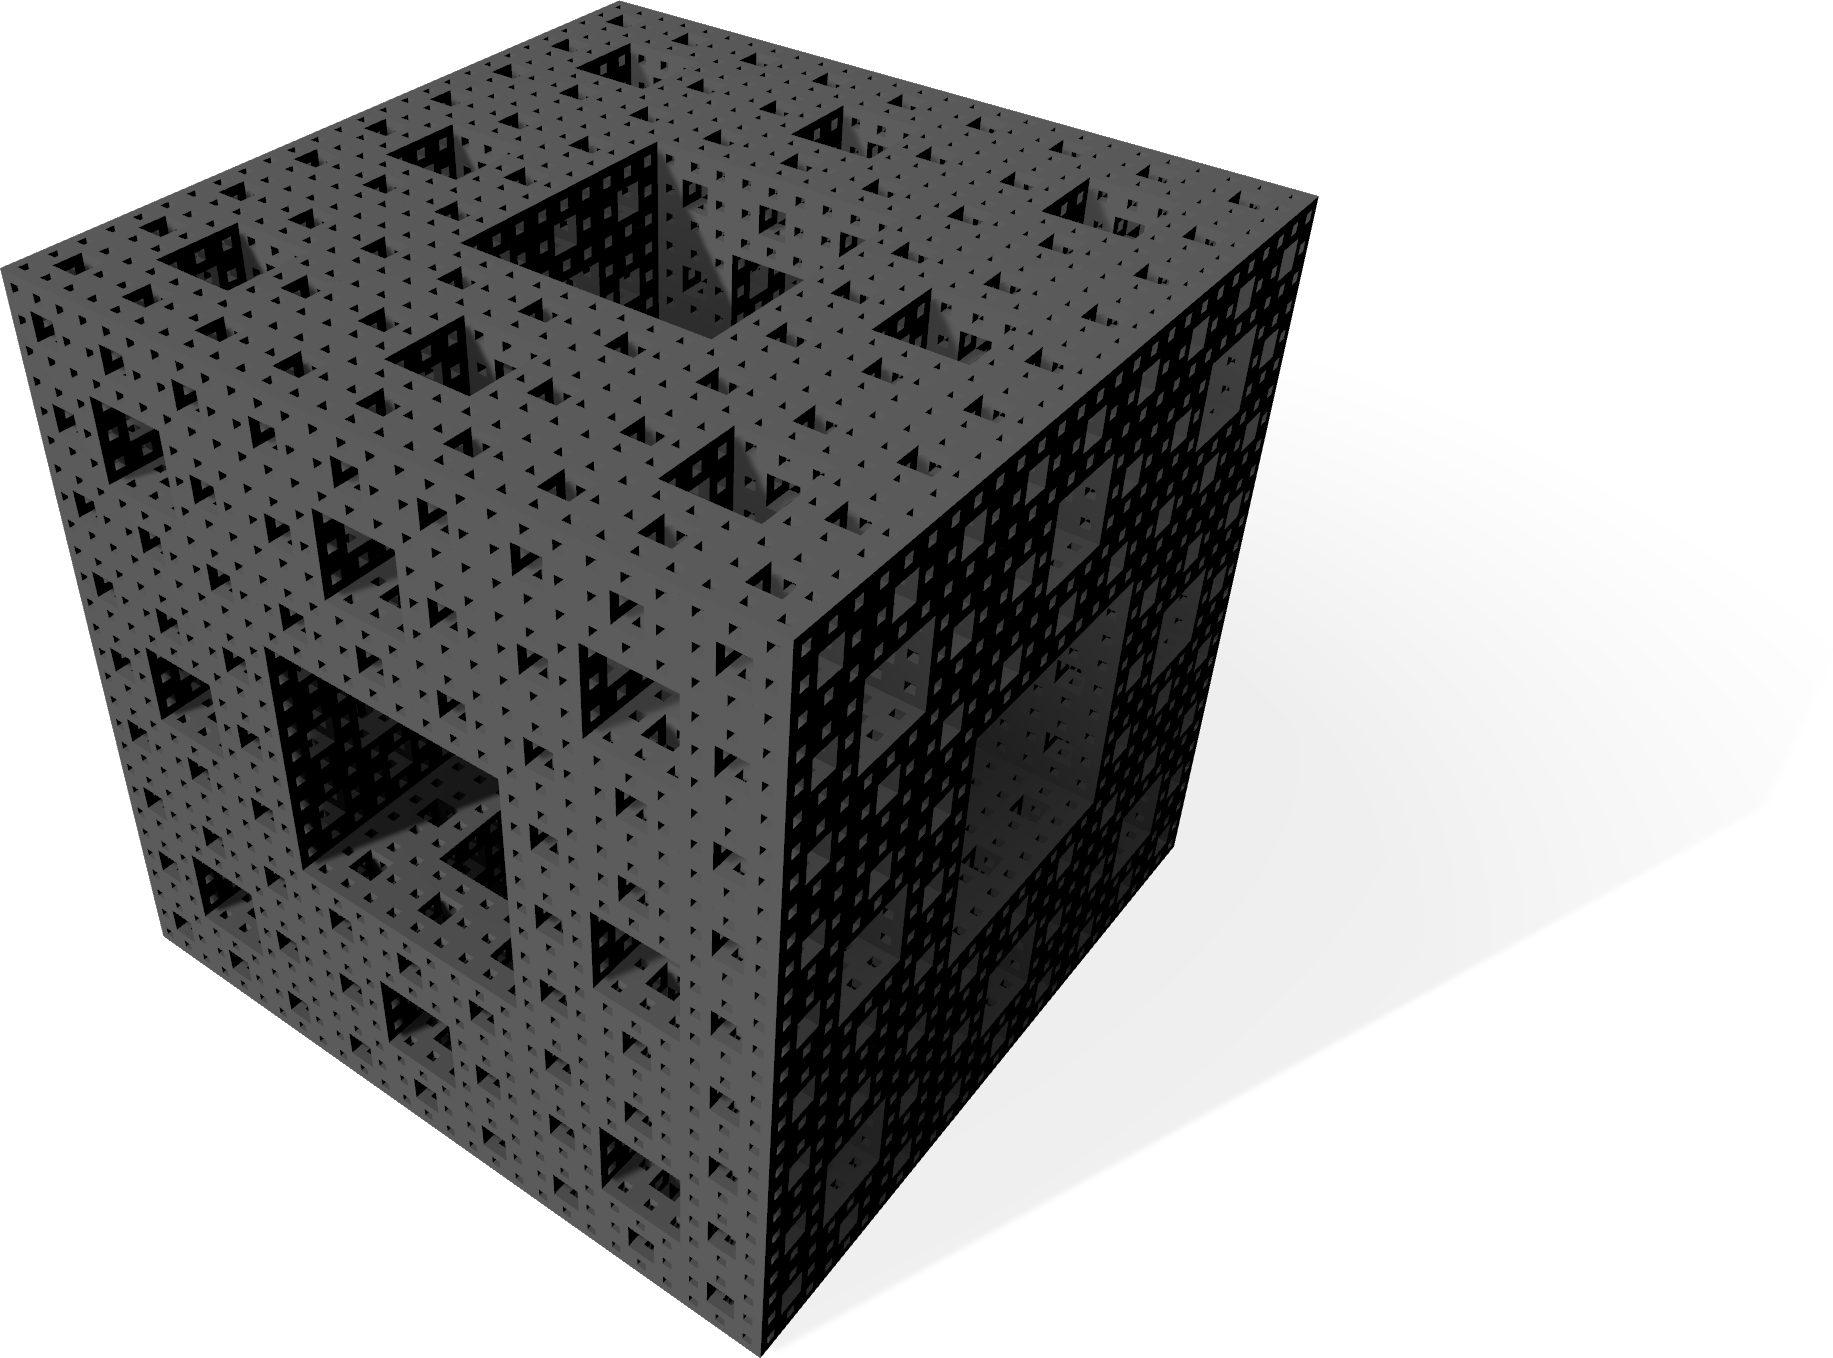
\includegraphics[width=5cm]{MengerSponge}
		\centering
		\captionsetup{justification=centering}
		\caption{Menger Sponge\\ 3D Model (4 steps)}
		\label{fig:MengerSponge}
	\end{subfigure}
	\begin{subfigure}{.24\textwidth}
		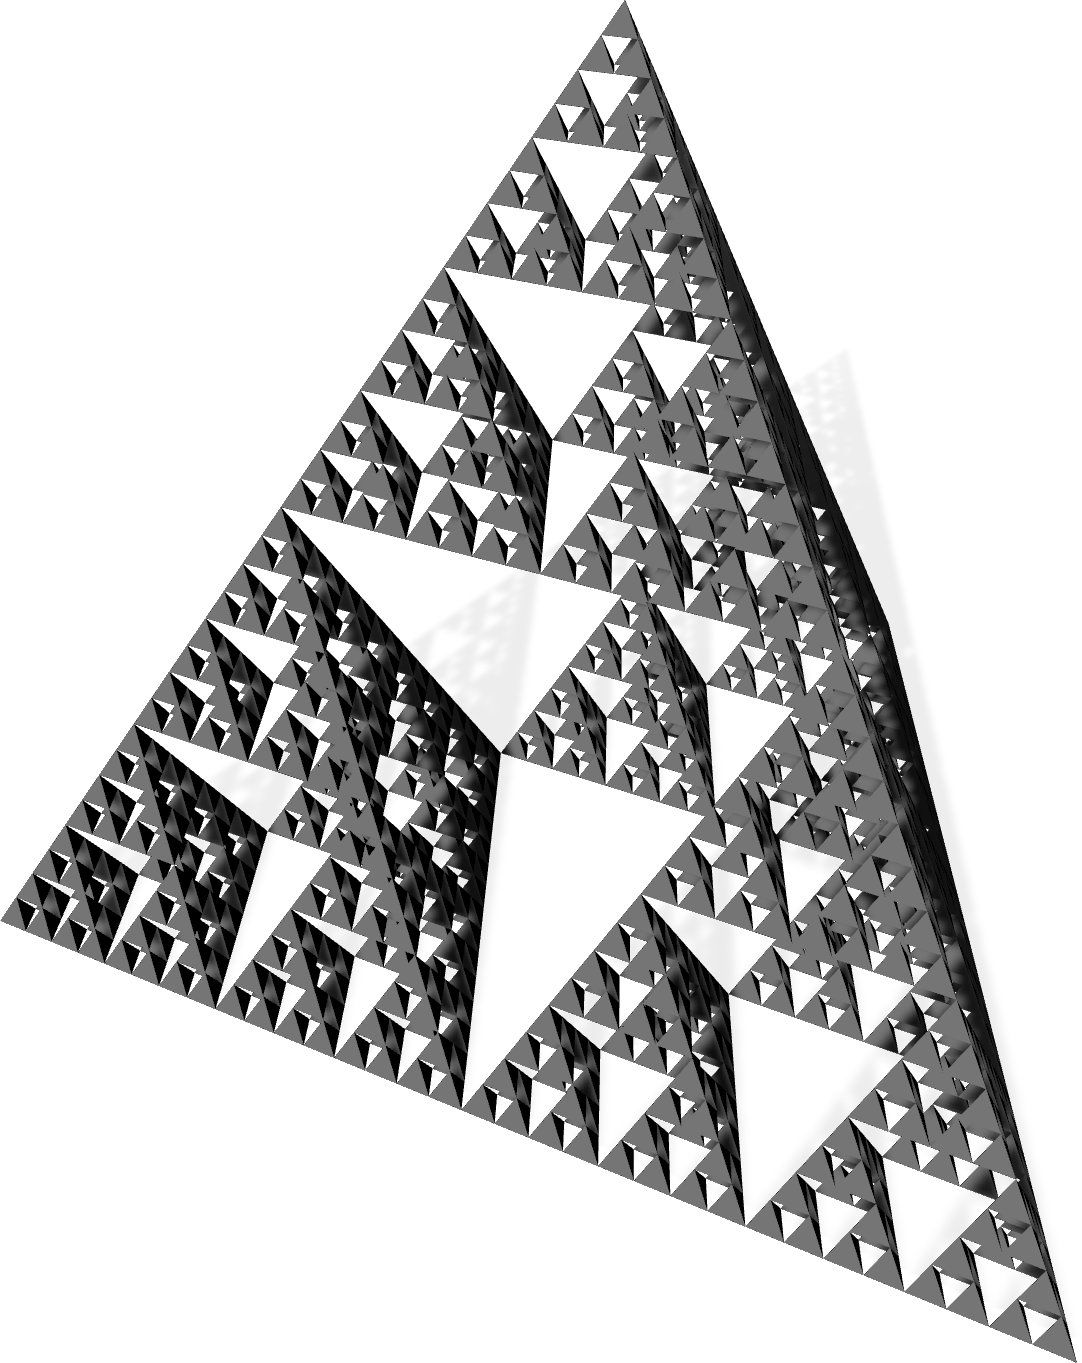
\includegraphics[width=3.5cm]{SierpinskiTetrahedron}
		\centering
		\captionsetup{justification=centering}
		\caption{Sierpiński Tetrahedron\\ 3D Model (5 steps)}
		\label{fig:SierpinskiTetrahedron}
	\end{subfigure}
	\begin{subfigure}{.24\textwidth}
		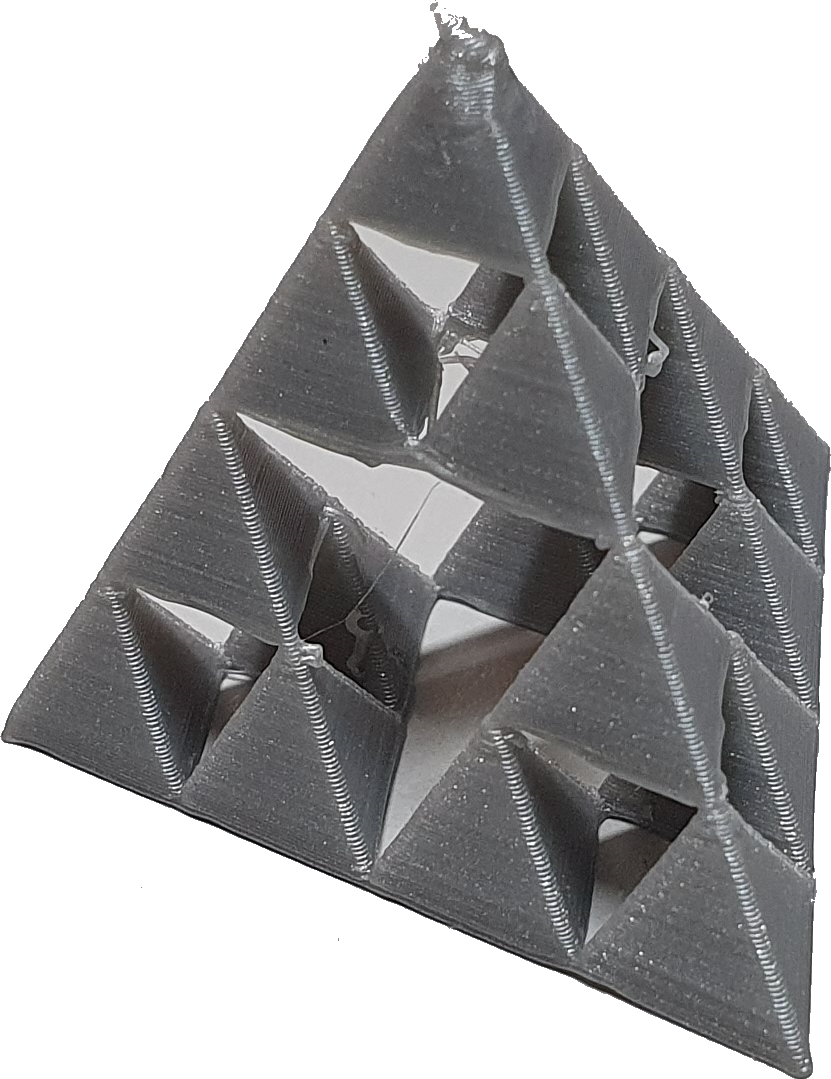
\includegraphics[width=2.8cm]{SierpinskiTetrahedronPhysics}
		\centering
		\captionsetup{justification=centering}
		\caption{Sierpiński Tetrahedron\\ 3D Printed (2 steps)}
		\label{fig:SierpinskiTetrahedron3Dprinted}
	\end{subfigure}
	\caption{Sierpiński 3D Fractals}
	\label{fig:Sierpinski3D}
\end{figure}

\subsection{Coastline of Islands}\label{appendix:coastlines}
The coastline can be measured at different scales.
As the scale is refined, one measures a more detailed curve, which leads to a larger length.
This refinement can be done indefinitely: from segments of $1000km$ (one would only capture the rough coastline shape) to segments of $1mm$ (one would need to go around every grain of sand), and even further considering sub-atomic scales.

Following this reasoning, the (1D) length of coastlines is infinite.
It is in fact a fractal with dimension greater than one (but less than 2, as contained in a plane).

It is then possible to measure how disordered the coastline of an island is, by approximating its Hausdorff dimension.
This will be done macroscopically, using maps extracted from the Google Maps service.
In this paper, 3 islands will be considered: The United Kingdom, Iceland, and Madagascar.
The United Kingdom and Iceland are understood as having irregular coastlines (so should have a high Hausdorff dimension), whereas Madagascar is thought to have a rather smooth coastline (Hausdorff dimension close to one).

\begin{figure}[!h]
	\centering
	\begin{subfigure}{.33\textwidth}
		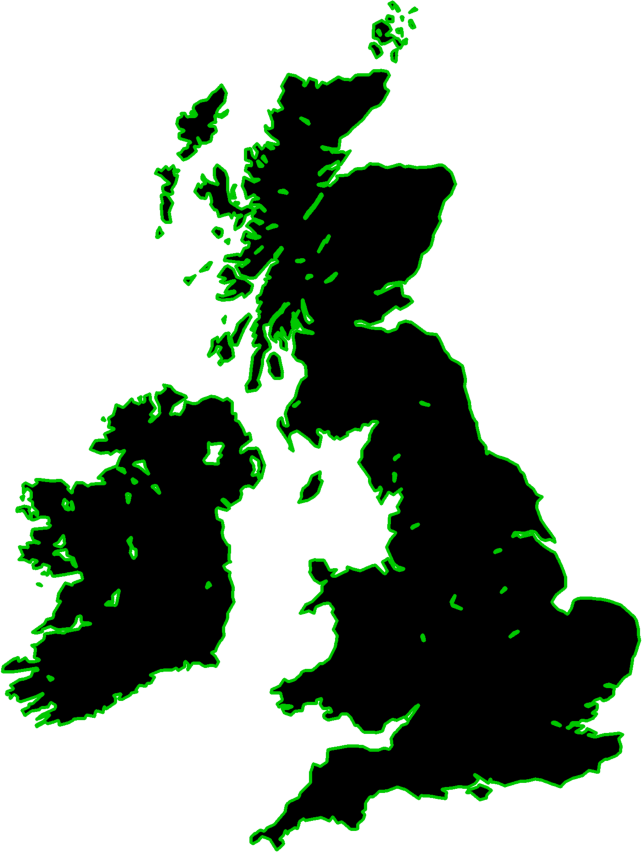
\includegraphics[scale=0.6]{UKCoastlines}
		\centering
		\captionsetup{justification=centering}
		\caption{United Kingdom}
		\label{fig:UKCoastlines}
	\end{subfigure}
	\begin{subfigure}{.33\textwidth}
		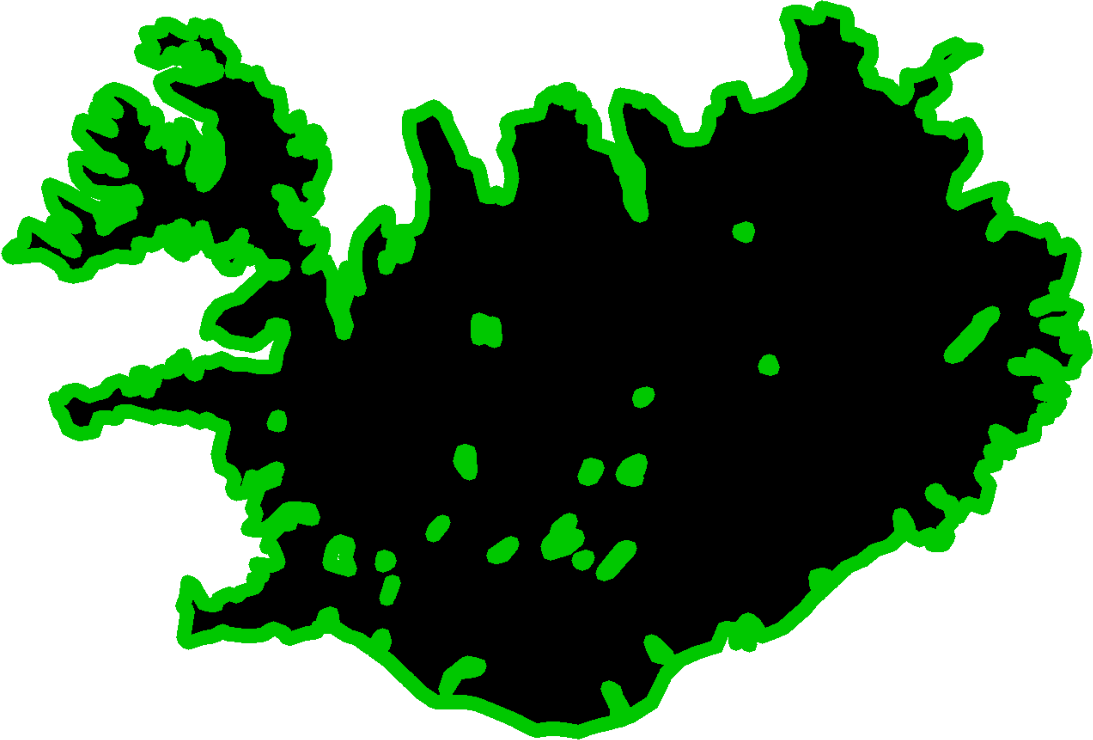
\includegraphics[scale=0.4]{IcelandCoastlines}
		\centering
		\captionsetup{justification=centering}
		\caption{Iceland}
		\label{fig:IcelandCoastlines}
	\end{subfigure}
	\begin{subfigure}{.30\textwidth}
		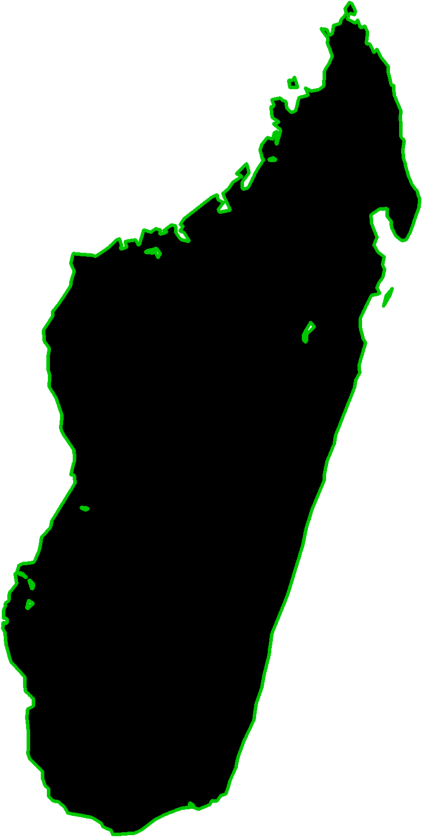
\includegraphics[scale=0.5]{MadagascarCoastlines}
		\centering
		\captionsetup{justification=centering}
		\caption{Madagascar}
		\label{fig:MadagascarCoastlines}
	\end{subfigure}
	\caption{Coastlines (coloured in green).}
	\label{fig:islandsCoastlines}
\end{figure}

Of course, the fractal dimension can only be an approximation.
We approach the problem as follows:
First, we take a high resolution map of the island, and split it into a binary colour image, black for the ground, and white for the surrounding sea (as in fig. \ref{fig:islandsCoastlines}).
Then, we reduce the size of the image by merging pixels ("pixelizing") to obtain lower resolution images.
The resolution panel will correspond to the measuring scales panel.
A subset of the resulting images is shown in fig. \ref{fig:islandsScales}.

\begin{figure}[!h]
	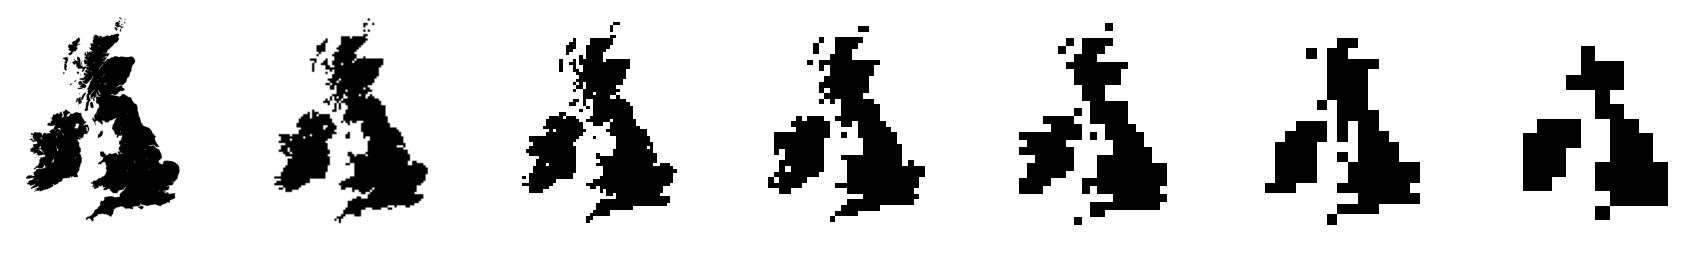
\includegraphics[width=15cm]{UKScales}\\
	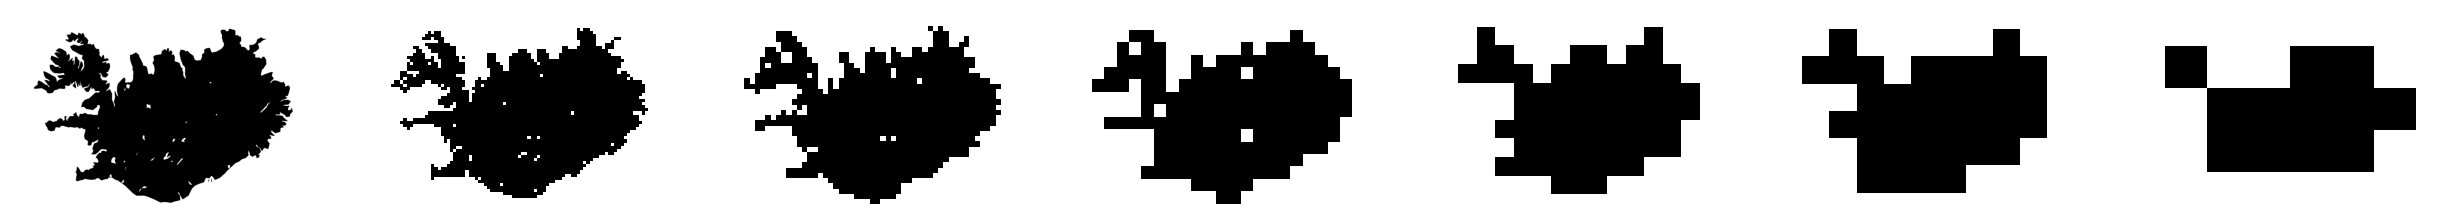
\includegraphics[width=15cm]{IcelandScales}\\
	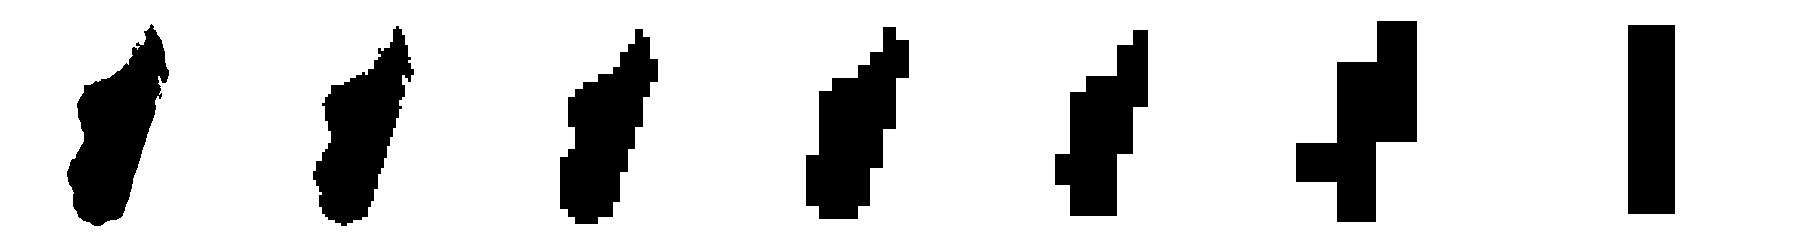
\includegraphics[width=15cm]{MadagascarScales}
	\centering
	\caption{Map scales for the UK, Iceland, and Madagascar.}
	\label{fig:islandsScales}
\end{figure}

Now, using computer vision (as a Python package), we obtain the contours of the shape in an image.
It is then straightforward to measure the length of the contour (in pixels, which can be converted to kilometres as we know the scale of the image).
Repeating this operation for each scale of the map gives an array of coastline length with associated scales.

Plotting the values in a log-log plot shows a nearly straight line; the approximate dimension will be given by the slope of the best fitting line.
We obtained the following dimensions:\\
\begin{tabular}{l l}\label{table:islandsDimensionRegression}
	\textbf{United Kingdom} & $D \approx 1.2354$ \\
	\textbf{Iceland}        & $D \approx 1.2466$ \\
	\textbf{Madagascar}     & $D \approx 1.0600$
\end{tabular}

The fitting line is very close to the data (see fig. \ref{fig:islandsDimensionRegression}), showing that the behaviour is as expected.

\begin{figure}[!h]
	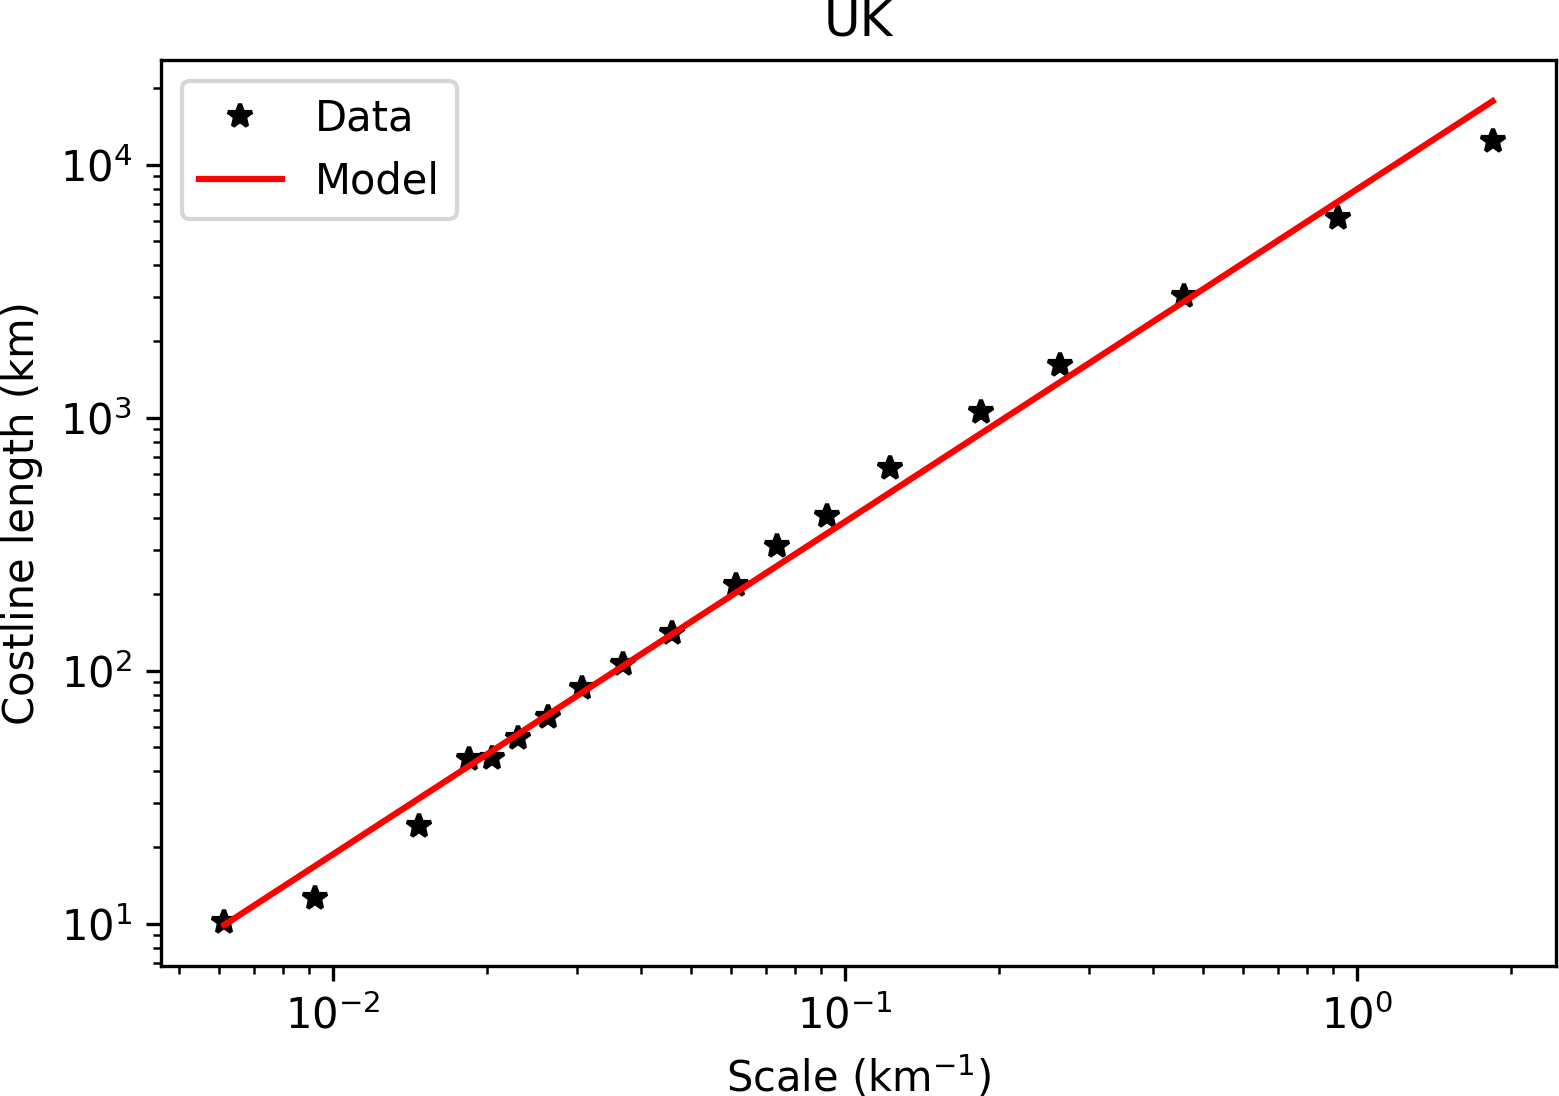
\includegraphics[width=5.25cm]{UKDimensionRegression}
	\hspace{0.25cm}
	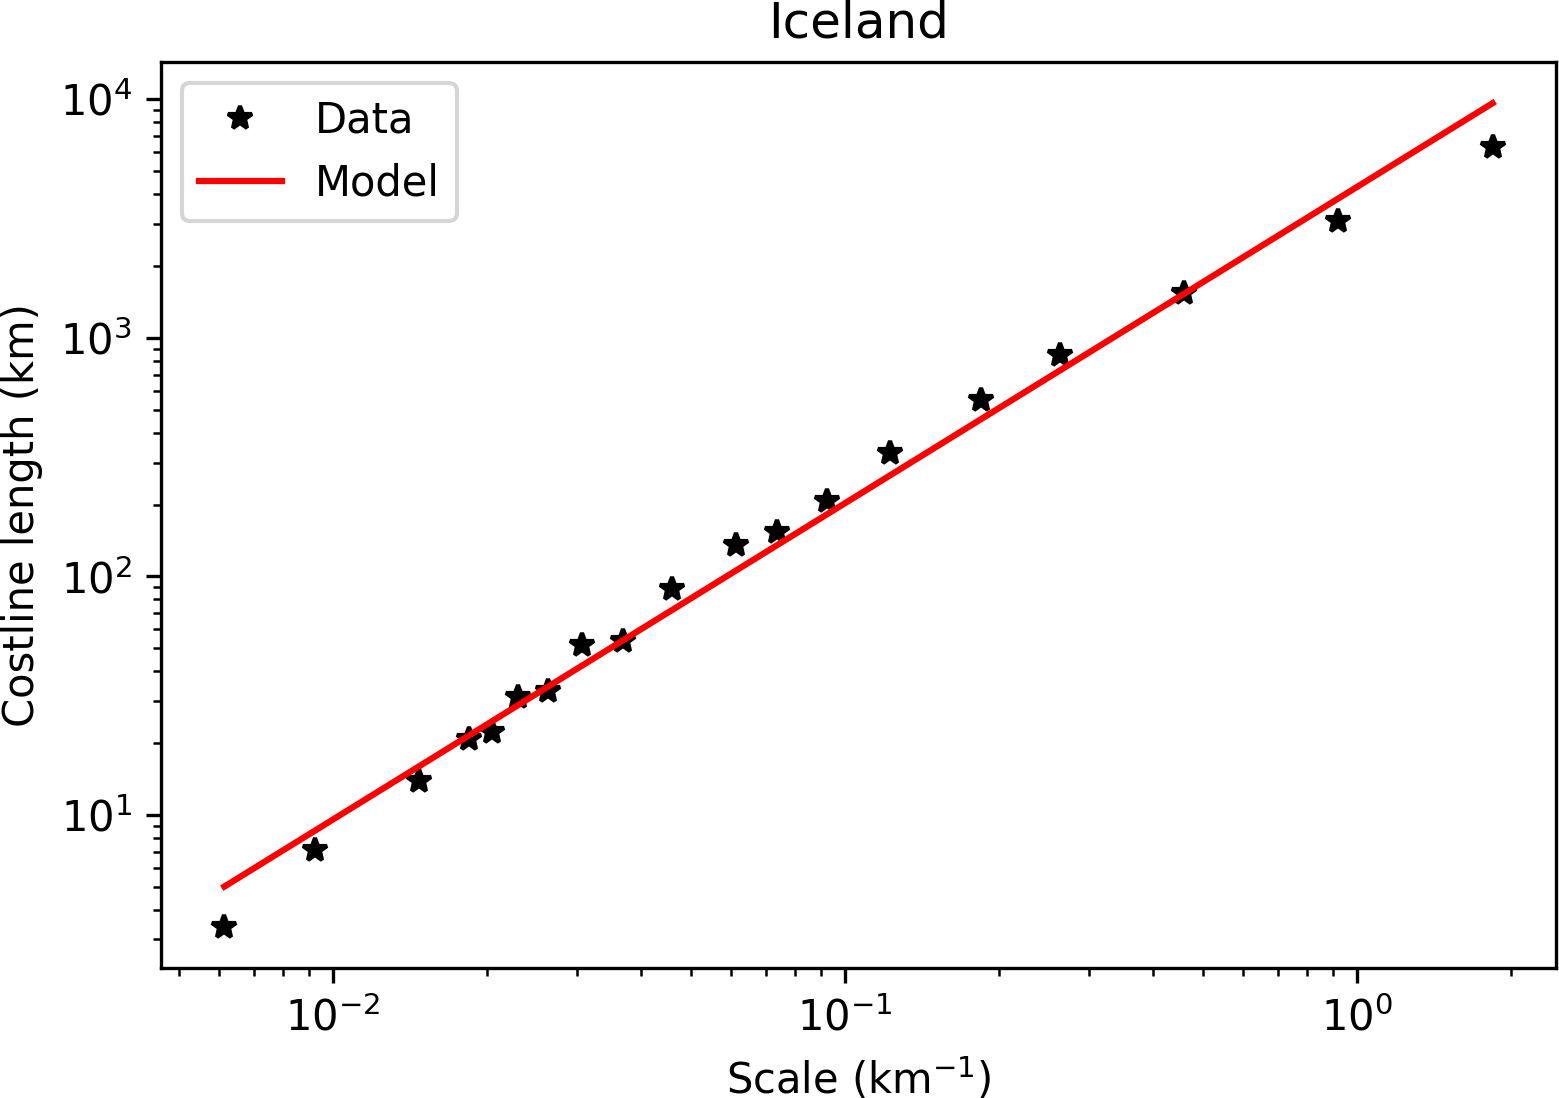
\includegraphics[width=5.25cm]{IcelandDimensionRegression}
	\hspace{0.25cm}
	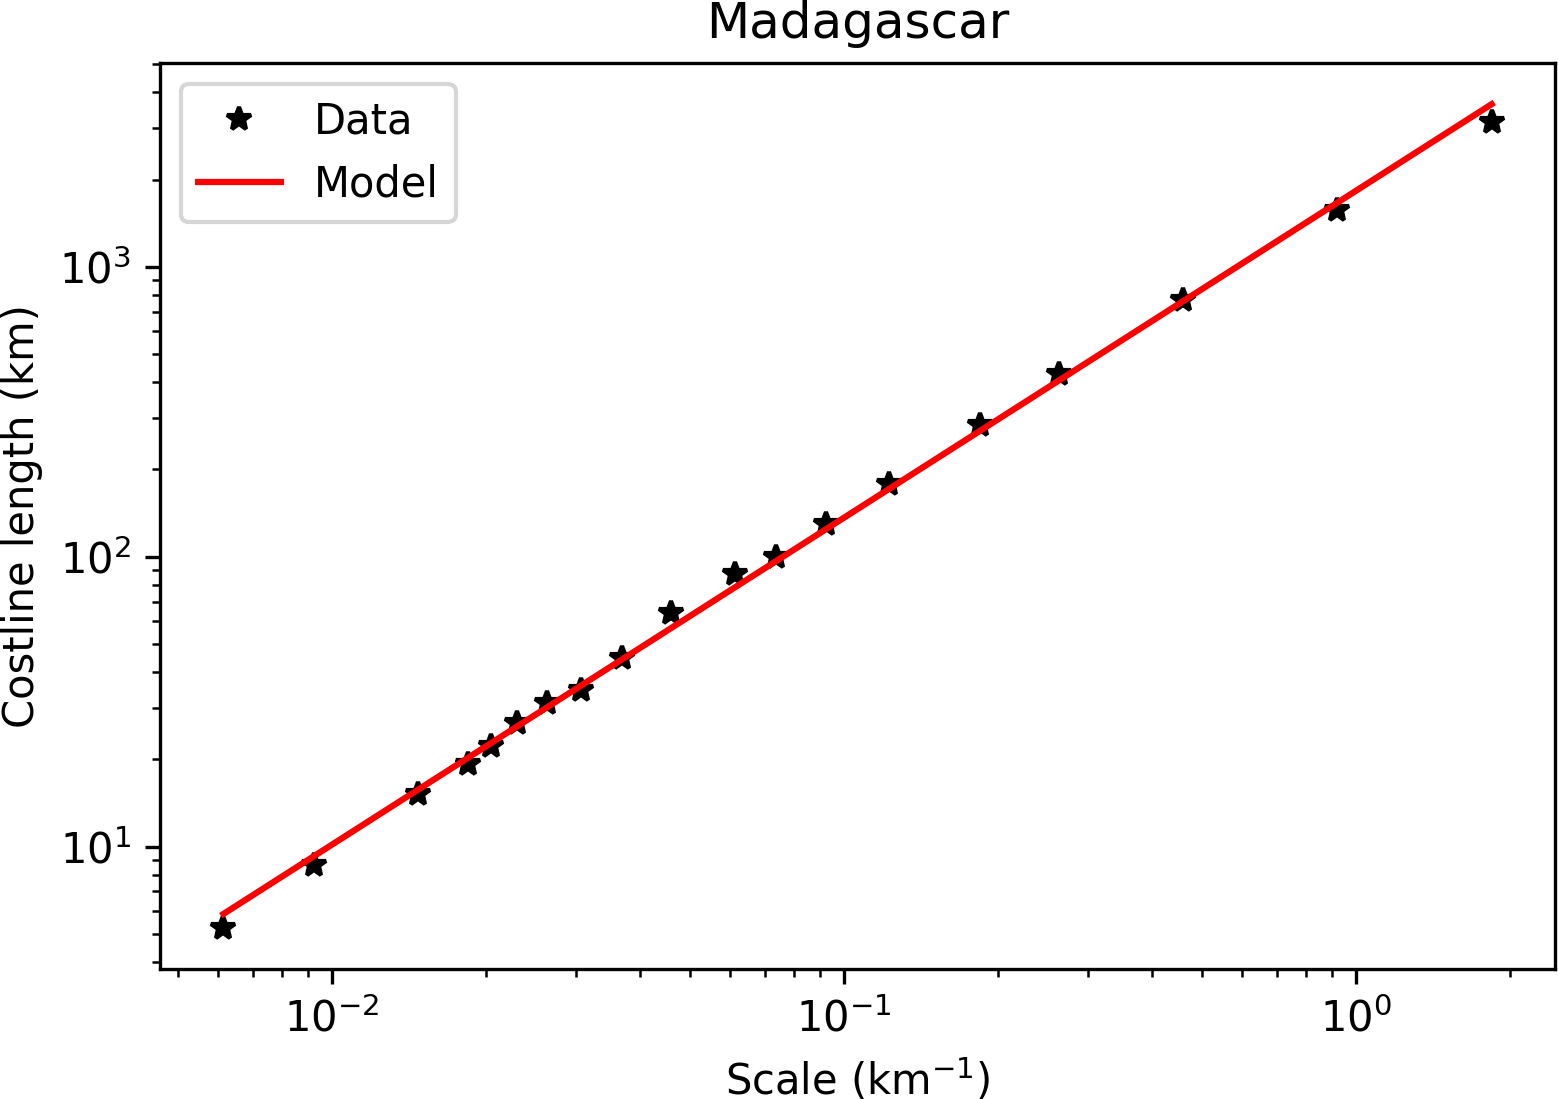
\includegraphics[width=5.25cm]{MadagascarDimensionRegression}
	\centering
	\caption{Islands Dimension Regression}
	\label{fig:islandsDimensionRegression}
\end{figure}

The full code for this study can be found here: \url{https://colab.research.google.com/drive/1qo8S8oxqcLsw9UFrq5wTuVyxVA48uwFF?usp=sharing}.


	% !TeX spellcheck = en_GB
\section{Finding Crossings}
Percolations are complicated objects.
Even for finite percolations, say one with side $n$, depth $d$ in $D$ dimensions, here are $2^{\left( n^D \right)^d}$ possibilities.
This grows extremely rapidly, and makes theoretical results hard to derive.

Therefore, we choose to study these object further with numerical simulations.

\subsection{Examples}
To see how complicated finding crossing on percolation becomes when $d$ grows, we look at some examples in two dimensions ($D=2$), with sides $n=2,3,5$ (see fig. \ref{fig:crossingExPerc2}, \ref{fig:crossingExPerc3}, \ref{fig:crossingExPerc5}).
\begin{figure}[!h]
	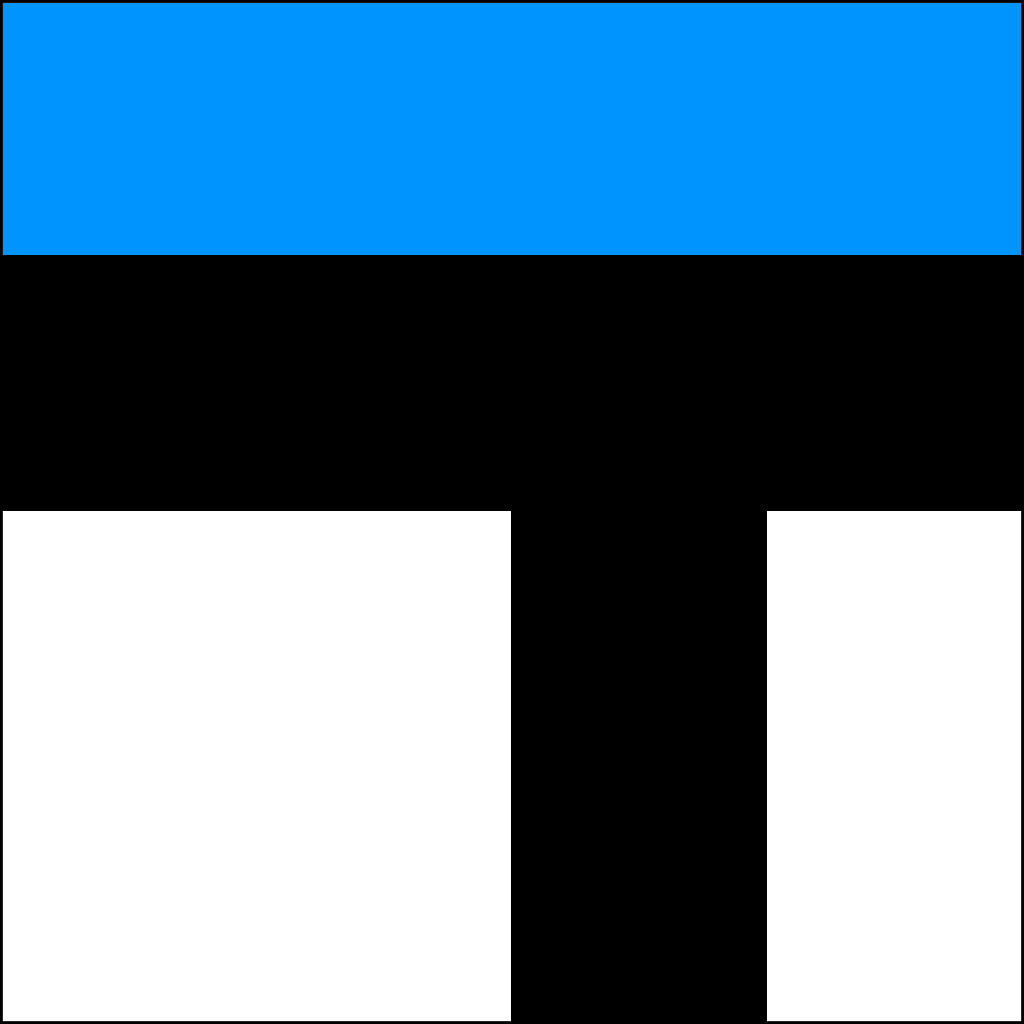
\includegraphics[width=3.1cm]{crossing-ex_perc2step2}
	\hspace{0.1cm}
	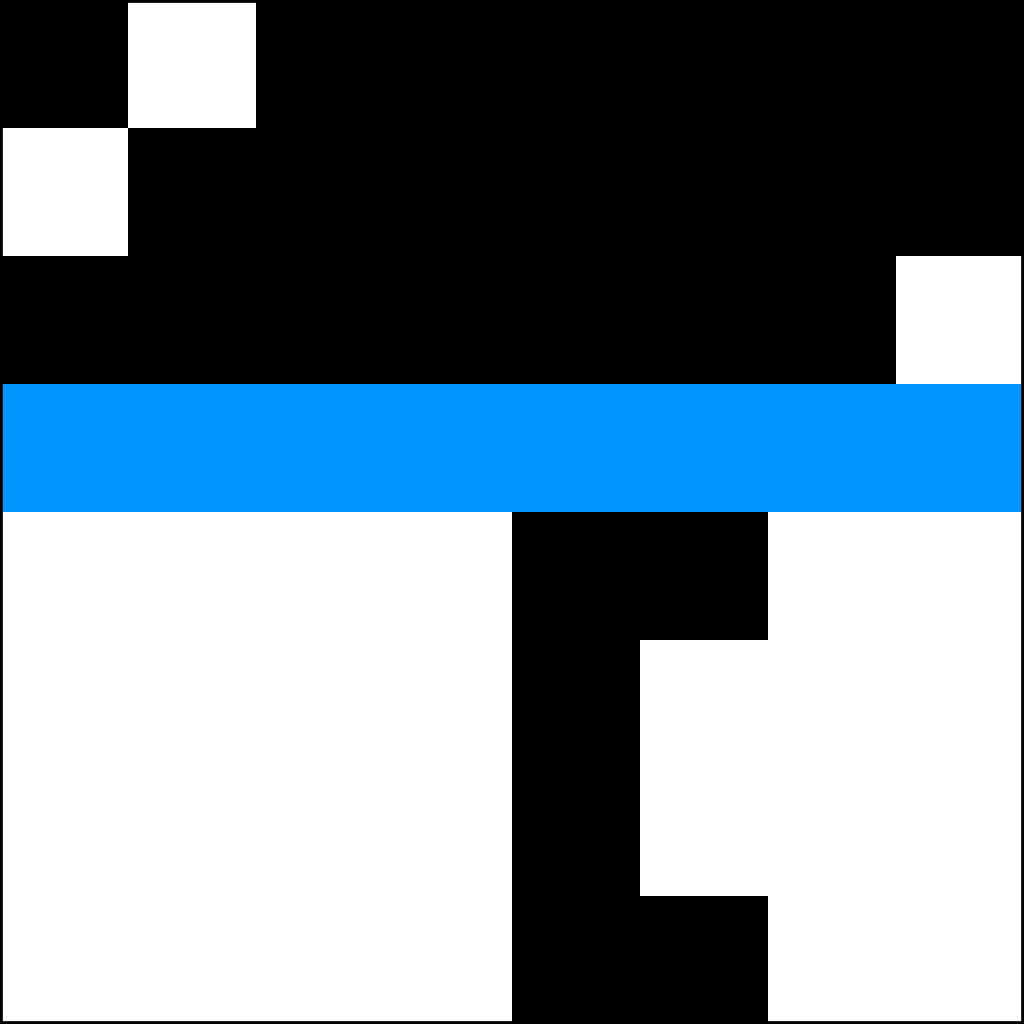
\includegraphics[width=3.1cm]{crossing-ex_perc2step3}
	\hspace{0.1cm}
	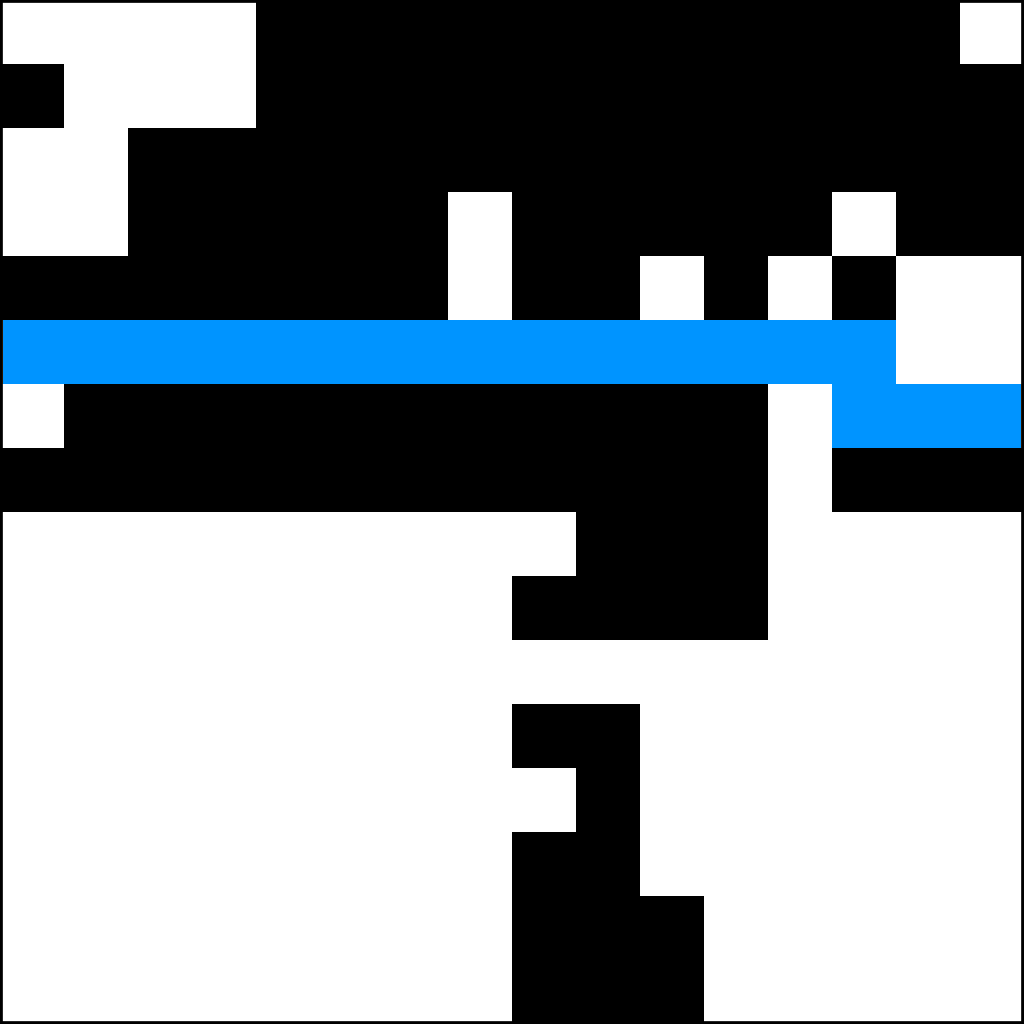
\includegraphics[width=3.1cm]{crossing-ex_perc2step4}
	\hspace{0.1cm}
	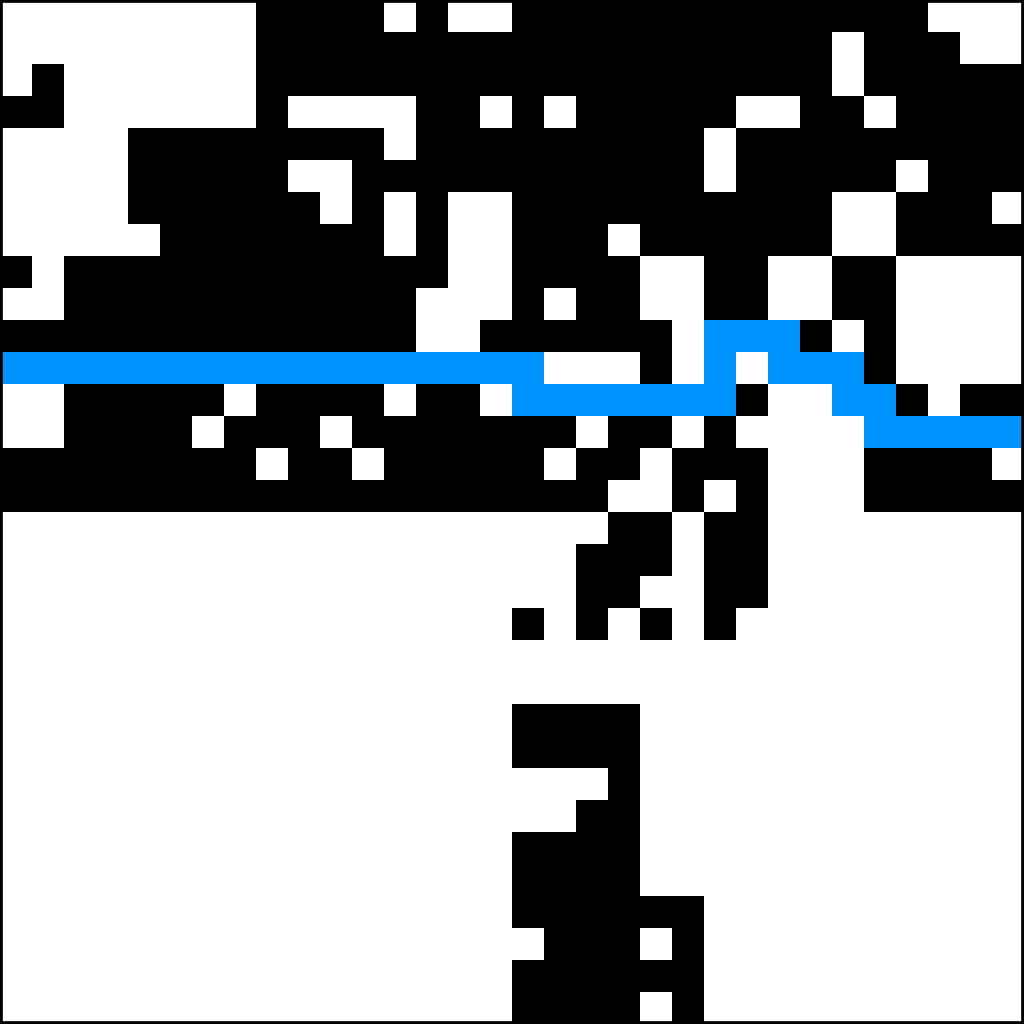
\includegraphics[width=3.1cm]{crossing-ex_perc2step5}
	\hspace{0.1cm}
	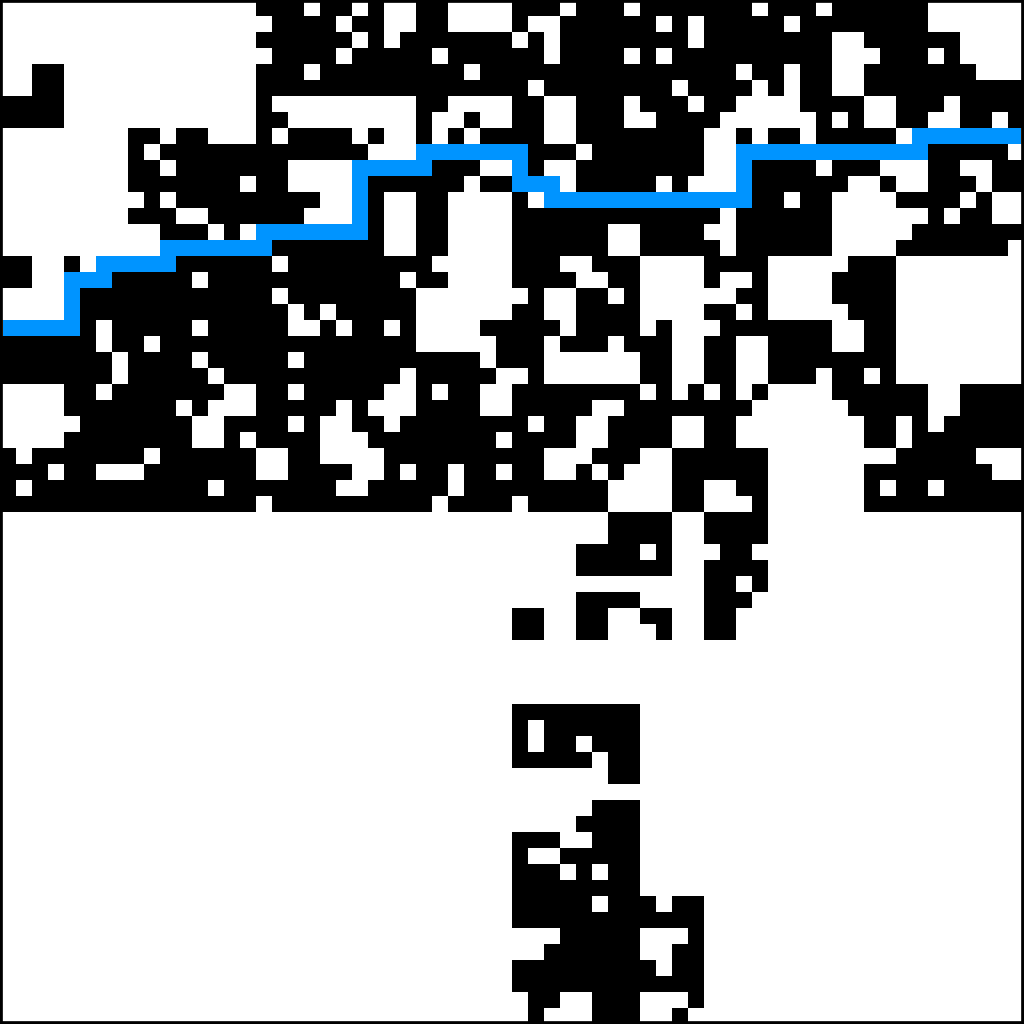
\includegraphics[width=3.1cm]{crossing-ex_perc2step6}
	\centering
	\caption{Crossings for a percolation with side $n=2$, at depths $k=2,3,4,5,6$.}
	\label{fig:crossingExPerc2}
\end{figure}
\begin{figure}[!h]
	
\includegraphics[width=4cm]{crossing-ex_perc3step1}
	\hspace{0.1cm}
	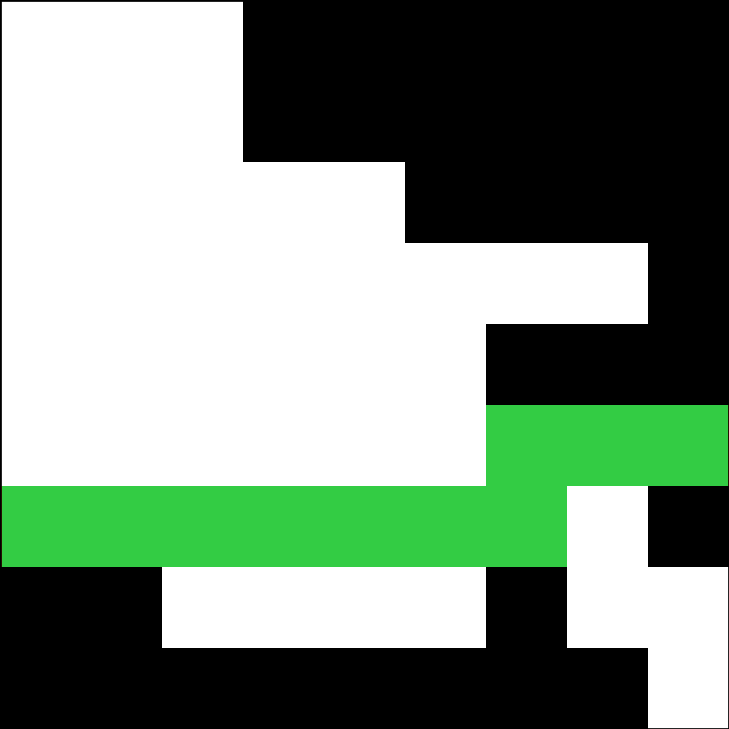
\includegraphics[width=4cm]{crossing-ex_perc3step2}
	\hspace{0.1cm}
	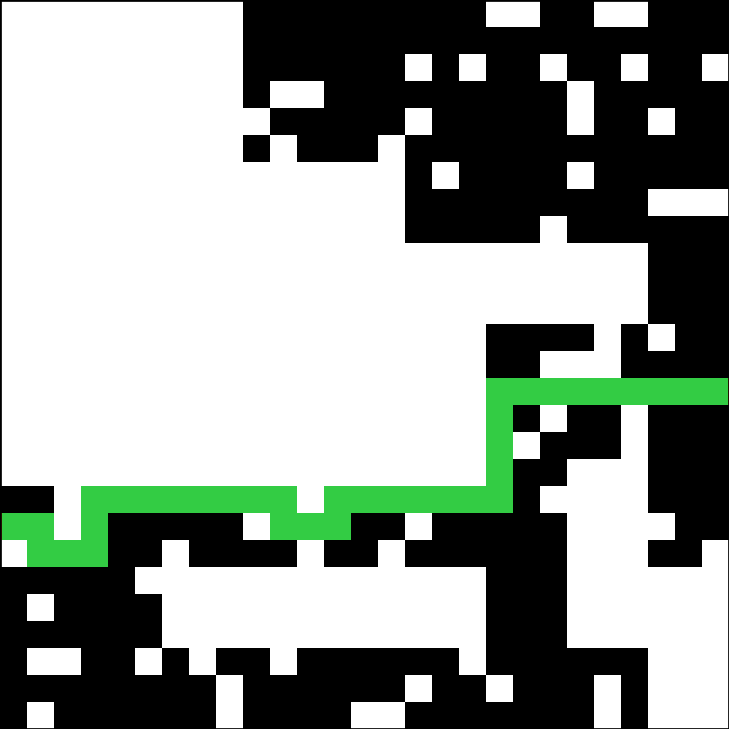
\includegraphics[width=4cm]{crossing-ex_perc3step3}
	\hspace{0.1cm}
	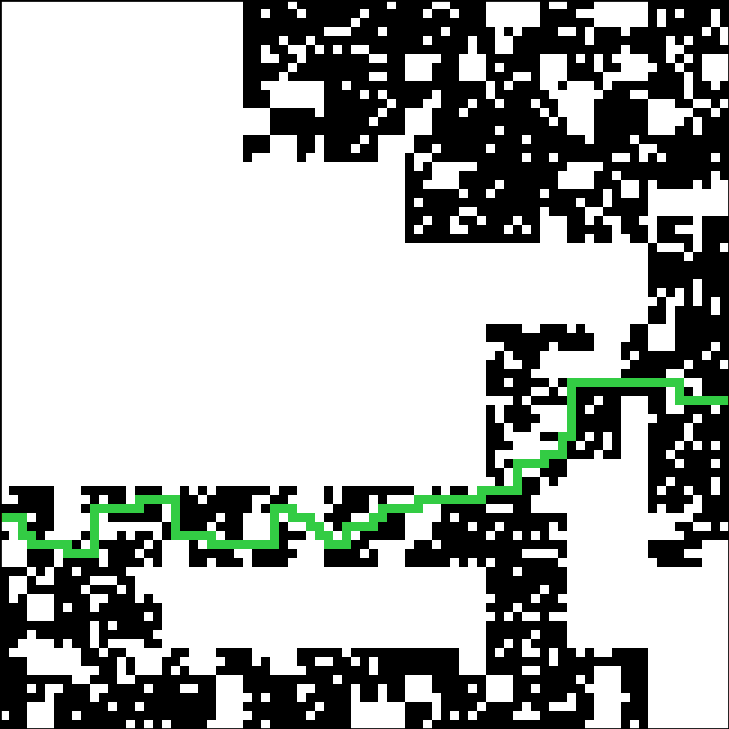
\includegraphics[width=4cm]{crossing-ex_perc3step4}
	\centering
	\caption{Crossings for a percolation with side $n=3$, at depths $k=1,2,3,4$.}
	\label{fig:crossingExPerc3}
\end{figure}
\begin{figure}[!h]
	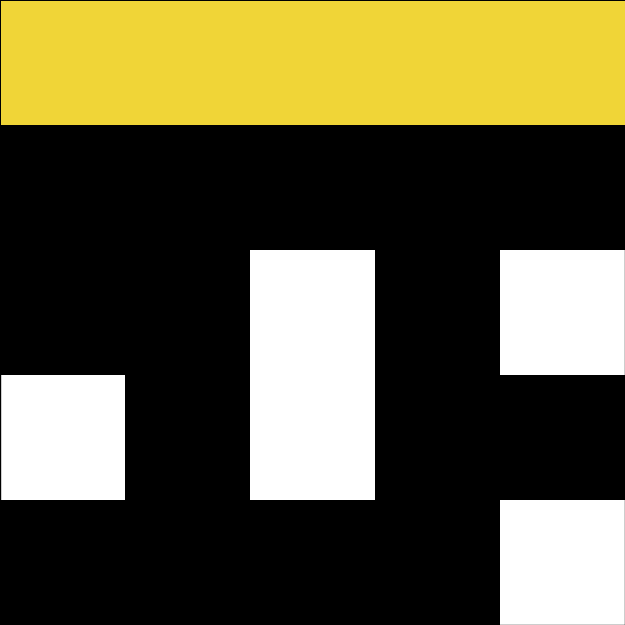
\includegraphics[width=4.9cm]{crossing-ex_perc5step1}
	\hspace{0.9cm}
	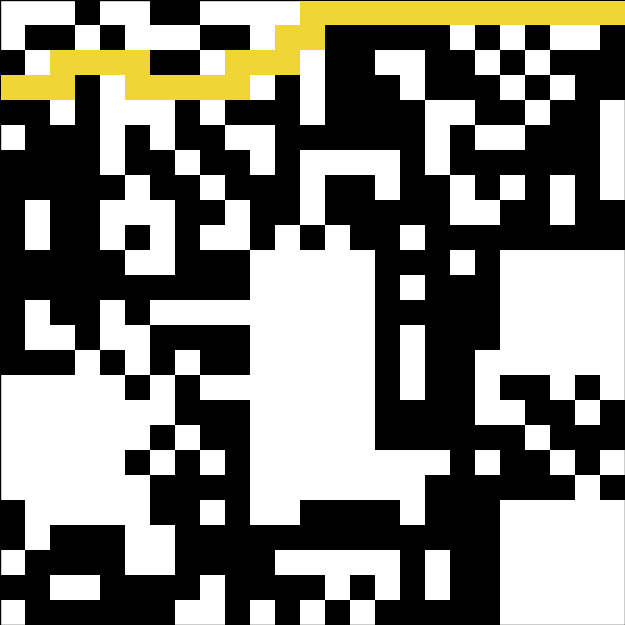
\includegraphics[width=4.9cm]{crossing-ex_perc5step2}
	\hspace{0.9cm}
	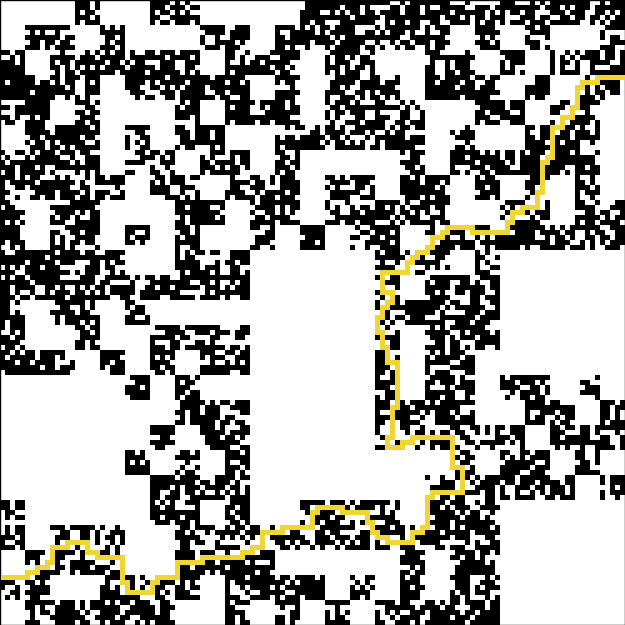
\includegraphics[width=4.9cm]{crossing-ex_perc5step3}
	\centering
	\caption{Crossings for a percolation with side $n=5$, at depths $k=1,2,3$.}
	\label{fig:crossingExPerc5}
\end{figure}

\subsection{Algorithms}
\paragraph{Percolations}
As (recursive) percolations are generated through a recursive process, it is logical (and elegant) to use a recursive function to generate them computationally.
We will represent a (finite) percolation $P \sim \text{Perc}^D(n,p,d)$ with a binary $D$-dimensional array of length $n^d$ in each dimensions.
Note that $D$ is a super-parameter.

This algorithm is given in pseudocode in algorithm \ref{algo:percolationGeneration}. Julia implementations
\footnote{2D percolation Julia implementation: \url{https://github.com/pauldubois98/PercolationFractalsStudy/blob/main/fractal\_percolation2D.jl}}
\footnote{3D percolation Julia implementation: \url{https://github.com/pauldubois98/PercolationFractalsStudy/blob/main/fractal\_percolation3D.jl}}
(used later in simulations for empirical estimations) can be found on the GitHub repository
\footnote{See \url{https://github.com/pauldubois98/PercolationFractalsStudy}.}.

\begin{algorithm}[!h]
	\caption{Percolation generation algorithm}\label{algo:percolationGeneration}
	\begin{algorithmic}[1]
		\State{\textit{Fills the $\left[ i_1,i_1+n^k\right] \times \cdots \times \left[ i_D,i_D+n^k\right]$ sub-array of $P$.}}
		\Procedure{percolationFill$^D$}{$P, \ i_1,\dots,i_D, \ n, p, k$}
		\If{$k = 0$}
		\State $P[i_1,\dots,i_D] \gets \textbf{random}()\footnotemark < p$ \Comment{stop recursion}
		\Else
		\For{$0 \leq j_1,\dots,j_D < n$}
		\If{$\textbf{random}() < p$}
		\State $\textsc{percolationFill}(P, \ i_1+(j_1 n^k),\dots,i_D+(j_D n^k), \ n, p, k-1)$ \Comment{recursion}
		\Else
		\State $P[i_1:i_1+n^k,\dots,i_D:i_D+n^k] \gets \textbf{zeros$^D$}(n^k,\dots,n^k)$ \Comment{void cells}
		\EndIf
		\EndFor
		\EndIf
		\EndProcedure
		\State{\textit{Generates a percolation $P \sim \text{Perc}^D(n,p,d)$.}}
		\Procedure{percolation$^D$}{$n, p, d$}
		\State $P \gets \textbf{init$^D$}(n^d,\dots,n^d)$
		\State $\textsc{percolationFill}(P, \ i_1,\dots,i_D, \ n, p, d)$ \Comment{fill $P$ recursively}
		\State \textbf{return} $P$
		\EndProcedure
	\end{algorithmic}
\end{algorithm}
\addtocounter{footnote}{-1}
\stepcounter{footnote}\footnotetext{$\textbf{random}()$ generates a random number $x \sim \mathcal{U}(0,1)$\footnotemark.}
\addtocounter{footnote}{-1}
\stepcounter{footnote}\footnotetext{Writing $x \sim \mathcal{U}(a,b)$ for $x$ a random variable with uniform distribution on $\left[ a,b \right]$.}

\paragraph{Crossings}\label{crossingAlgorithm}
Given a percolation, it is not clear how to proceed on the task of determining if a crossing exists.

Our approach of the problem is rather unusual.

We simulate a "fire" propagating from one side of the cuboid, and check if it reaches the other side.\footnote{This is inspired by simulations of forest fires from the game "The Pyromaniac Game"\cite{pyromaniacGame}.}
If it does, then a crossing exists, otherwise, no crossing exists.
The rules of propagation for the fire (materialized by active cells\footnote{We call a "cell" one of the $D$ dimensional cuboids of side $\nicefrac{1}{n^d}$}) are as follows:
\begin{enumerate}
	\item If a cell is active at time $t$, then the non-empty adjacent cells become active at time $t+1$.
	\item If a cell is active at time $t$, it deactivates and can no longer be active on times $\tilde{t}>t$.
\end{enumerate}
At the beginning ($t=0$), we set all the non-empty cells from one side of the unit cuboid as active cells.
As soon as a cell from the opposite side of the unit cuboid is active, a path has been found (the time $t$ even gives the length of the crossing), and this is the shortest crossing.
If at some time $t$, no cell is active and no crossing was found before (i.e. the blaze turns off before reaching the other side), then no crossing exist.

Note that this technique tells us if there is a crossing, and what is the minimal length. However, it does not give the crossing path explicitly.
To find it, one needs to save the set of active cells at each time, and propagate backwards.

This algorithm \ref{algo:crossingFinding} is a pseudocode implementation of this process.
Julia implementations
\footnote{2D crossing Julia implementation: \url{https://github.com/pauldubois98/PercolationFractalsStudy/blob/main/crossings2D.jl}}
\footnote{3D crossing Julia implementation: \url{https://github.com/pauldubois98/PercolationFractalsStudy/blob/main/crossings3D.jl}}
(used for empirical probability approximation) can be found again on the GitHub repository
\footnote{See \url{https://github.com/pauldubois98/PercolationFractalsStudy}.}.

Visualisation of this algorithm:
\begin{itemize}
	\item In 2D: \url{https://pauldubois98.github.io/PercolationFractalsAlgorithmsDemo/2Dcrossing/index.html}
	\item In 3D: \url{https://pauldubois98.github.io/PercolationFractalsAlgorithmsDemo/3Dcrossing/index.html}
\end{itemize}

\begin{algorithm}[!h]
	\caption{Crossing finding algorithm}\label{algo:crossingFinding}
	\begin{algorithmic}[1]
		\State{\textit{Perform one step propagation on $A$, with respect to $P$}}
		\Procedure{neighbors$^D$}{$A,\, P, \ n,d$}
		\State $B \gets \textbf{zeros$^D$}(n^d,\dots,n^d)$ \Comment{newly active cells}
		\For{$1 \leq i_1,\dots,i_D < n^d$}
		\If{$A[i_1,\dots,i_D]=2$}
		\State $B[i_1,\dots,i_D] = 2$ \Comment{remain inactive}
		\EndIf
		\If{$A[i_1,\dots,i_D]=1$}
		\State $B[i_1,\dots,i_D] = 2$ \Comment{deactivate cell}
		\For{$1 \leq j \leq D$}
		\If{$P[i_1,\dots,i_j-1,\dots,i_D]$ and $A[i_1,\dots,i_j-1,\dots,i_D] = 0$}
		\State $B[i_1,\dots,i_j-1,\dots,i_D] \gets 1$ \Comment{activate cell}
		\EndIf
		\If{$P[i_1,\dots,i_j+1,\dots,i_D]$ and $A[i_1,\dots,i_j+1,\dots,i_D] = 0$}
		\State $B[i_1,\dots,i_j+1,\dots,i_D] \gets 1$ \Comment{activate cell}
		\EndIf
		\EndFor
		\EndIf
		\EndFor
		\State \textbf{return} $B$
		\EndProcedure
		\State{\textit{Returns the length of the shortest crossing on percolation $P \sim \text{Perc}^D(n,p,d)$; returns $0$ if none exist.}}
		\Procedure{crossing$^D$}{$P,\ n,d$}
		\State $A \gets \textbf{zeros$^D$}(n^d,\dots,n^d)$ \Comment{active cells}
		\State $A[0,:,\dots,:] \gets P[0,:,\dots,:]$ \Comment{initialize active cells}
		\State $t \gets 0$
		\While{\textbf{any}($A=1$) and \textbf{any}($A[n^d,:,\dots,:]=1$)}
		\State $A \gets \textsc{neighbors}(P,A)$ \Comment{propagate one step}
		\State $t \gets t+1$
		\EndWhile
		\If{\textbf{any}$(A[n^d,:,\dots,:])$}
		\State \textbf{return} $t$
		\Else
		\State \textbf{return} $0$
		\EndIf
		\EndProcedure
	\end{algorithmic}
\end{algorithm}

By restricting the possible steps (not allowing activation to propagate backwards), this algorithm may be adapted to find semi-straight crossings (the above would give non-straight crossings).
It can also be used for straight crossings, but in this case, it is faster to sum the percolation array on the first dimension: a straight crossing exists if one of the sums gives $n^d$.

%implementation choices
	
\end{document}
